\documentclass{article}
%% 1. CÀI ĐẶT CƠ BẢN & LỚP VĂN BẢN
\usepackage[utf8]{inputenc}
% \usepackage[T5]{fontenc} % Bỏ dòng này vì đã có T1 bên dưới, tránh xung đột
\usepackage[T1]{fontenc}
\usepackage[table,xcdraw]{xcolor}
\usepackage{tikz}
\usepackage{tcolorbox}

%% 2. BỐ CỤC TRANG & CANH LỀ (ĐÃ SỬA THEO YÊU CẦU)
\usepackage[a4paper, top=3.5cm, bottom=3cm, left=3.5cm, right=2cm]{geometry}
% Đã BỎ tùy chọn "twoside" để lề trang không bị lệch


%% 3. NGÔN NGỮ, FONT CHỮ & ĐỊNH DẠNG ĐOẠN VĂN (ĐÃ SỬA THEO YÊU CẦU)
\usepackage[vietnamese]{babel}
\usepackage{mathptmx} % Font Times New Roman
\usepackage{indentfirst}
% --- CÀI ĐẶT FONT, GIÃN DÒNG, THỤT LỀ MỚI ---
\renewcommand{\normalsize}{\fontsize{13}{15.6}\selectfont}
\linespread{1.5} % Giãn dòng 1.5
\setlength{\parindent}{1cm} % Thụt đầu dòng 1cm
\setlength{\parskip}{10pt} % Khoảng cách giữa các đoạn là 10pt
\setlength{\emergencystretch}{2em}


%% 4. TÙY CHỈNH CÁC CẤP ĐỀ MỤC (SECTION, SUBSECTION,...)
\usepackage{titlesec}
\setcounter{secnumdepth}{4}

% Định dạng cho các chương CÓ ĐÁNH SỐ 
\titleformat{\section}[block]
  {\fontsize{16pt}{0pt}\selectfont \bfseries \centering}
  {CHƯƠNG \thesection:}
  {0.5em}
  {}
\titlespacing*{\section}{0pt}{0pt}{15pt}

% Định dạng cho các chương KHÔNG ĐÁNH SỐ
\titleformat{name=\section,numberless}[display]
  {\fontsize{16pt}{0pt}\selectfont \bfseries \centering}
  {}
  {0em}
  {}

% Định dạng cho các mục con
\titleformat*{\subsection}{\fontsize{14pt}{0pt}\selectfont \bfseries}
\titlespacing*{\subsection}{0pt}{3pt}{0pt}

\titleformat*{\subsubsection}{\fontsize{13pt}{0pt}\selectfont \bfseries \itshape}
\titlespacing*{\subsubsection}{0pt}{6pt}{0pt}

\titleformat*{\paragraph}{\fontsize{13pt}{0pt}\selectfont \itshape}
\titlespacing*{\paragraph}{0pt}{0pt}{0pt}

\titleformat{\paragraph}
  {\normalfont\fontsize{13pt}{0pt}\selectfont\itshape}
  {\theparagraph}
  {1em}
  {}
\titlespacing*{\paragraph}{0pt}{0.5ex plus 0.5ex minus .2ex}{0.5ex plus .2ex}


%% 5. HÌNH ẢNH, BẢNG BIỂU & CHÚ THÍCH (CAPTION)
\usepackage[nottoc]{tocbibind}
\usepackage{tocloft}
\setlength{\cftbeforesecskip}{6pt}
\setlength{\cftbeforesubsecskip}{2pt}
\setlength{\cftbeforesubsubsecskip}{1pt}

% Căn giữa các tiêu đề danh mục tương tự tiêu đề section gốc
\renewcommand{\cfttoctitlefont}{\hspace*{\fill}\fontsize{16pt}{0pt}\selectfont\bfseries}
\renewcommand{\cftaftertoctitle}{\hspace*{\fill}}
\renewcommand{\cftloftitlefont}{\hspace*{\fill}\fontsize{16pt}{0pt}\selectfont\bfseries}
\renewcommand{\cftafterloftitle}{\hspace*{\fill}}
\renewcommand{\cftlottitlefont}{\hspace*{\fill}\fontsize{16pt}{0pt}\selectfont\bfseries}
\renewcommand{\cftafterlottitle}{\hspace*{\fill}}
\usepackage{graphicx}
\usepackage{float}
\usepackage{longtable}
\usepackage{tabularx}
\usepackage{multirow}
\usepackage[font=normal]{caption}
\usepackage{array}

\renewcommand{\figurename}{\fontsize{12pt}{0pt}\selectfont Hình}
\captionsetup[figure]{labelsep=space}

\renewcommand{\tablename}{\fontsize{12pt}{0pt}\selectfont Bảng}
\captionsetup[table]{labelsep=space}

\newcolumntype{s}{>{\hsize=.3\hsize}X}
\newcolumntype{y}{>{\hsize=.4\hsize}X}
\newcolumntype{d}{>{\hsize=.1\hsize}X}
\newcolumntype{a}{>{\hsize=1.1\hsize}X}
\newcolumntype{g}{>{\hsize=5\hsize}X}
\newcolumntype{P}[1]{>{\raggedright\arraybackslash}p{#1}}
% --- SỬA LỖI TẠI ĐÂY ---
% \renewcommand{\tabularxcolumn}[1]{>{\small}m{#1}} % Dòng lệnh cũ gây lỗi thu nhỏ chữ
\renewcommand{\tabularxcolumn}[1]{>{\raggedright\arraybackslash}m{#1}} % Lệnh mới: Bỏ \small, thêm căn lề trái cho đẹp
% -----------------------


%% 6. KHỐI LỆNH (CODE LISTINGS) 
\usepackage{listings}
% Gói xcolor đã được nạp ở mục 5, không cần nạp lại

\lstdefinestyle{customcode}{
    basicstyle=\small\ttfamily,
    breaklines=true,
    numbers=left,
    numberstyle=\tiny\color{gray},
    keywordstyle=\color{blue!80!black}\bfseries,
    commentstyle=\color{green!50!black}\itshape,
    stringstyle=\color{red!70!black},
    showstringspaces=false,
    tabsize=2,
    captionpos=b,
    frame=single,
    rulecolor=\color{gray!40},
    xleftmargin=1.5em,
    framexleftmargin=1em,
    aboveskip=1.5em,
    belowskip=1.5em
}
\renewcommand{\lstlistingname}{Khối lệnh}


%% 7. TOÁN HỌC & CÁC MÔI TRƯỜNG ĐỊNH LÝ
\newtheorem{theorem}{Định lý}[section]
\newtheorem{defn}[theorem]{Định nghĩa}
\newtheorem{corollary}[theorem]{Hệ quả}
\newtheorem{lemma}[theorem]{Bổ đề}


%% 8. TÀI LIỆU THAM KHẢO
\usepackage[natbibapa]{apacite} 
\bibliographystyle{apacite}
\makeatletter
\def\APAC@apcfile{english.apc}
\makeatother

%% 9. CÁC GÓI BỔ SUNG KHÁC
\usepackage{wrapfig}
% Gói tikz đã được nạp ở mục 1, không cần nạp lại
\usetikzlibrary{calc,backgrounds}
\usepackage{soul}
\usepackage{colortbl}
\usepackage{forloop}
\usepackage{enumitem}

\definecolor{LightCyan}{rgb}{0.88,1,1}
\newcounter{loopcntr}
\newcommand{\rpt}[2][1]{\forloop{loopcntr}{0}{\value{loopcntr}<#1}{#2}}
\setitemize{itemsep=0pt,leftmargin=1.25cm,topsep = 3pt}


%% 10. ĐÁNH SỐ TỰ ĐỘNG & LIÊN KẾT 
\usepackage{chngcntr}
\usepackage[unicode, plainpages=false, pdfpagelabels=true, hidelinks]{hyperref}

% Cấu hình bộ đếm cho các môi trường
\counterwithin{figure}{section}
\counterwithin{table}{section}
\counterwithin{equation}{section}
% Các counter khác đã được article class và titlesec xử lý, không cần thêm


%% 11. ĐỊNH NGHĨA LẠI TÊN CÁC THÀNH PHẦN CỦA TÀI LIỆU
\AtBeginDocument{%
  \renewcommand{\contentsname}{MỤC LỤC}
  \renewcommand{\listfigurename}{DANH MỤC HÌNH VẼ}
  \renewcommand{\listtablename}{DANH MỤC BẢNG BIỂU}
  \renewcommand{\refname}{TÀI LIỆU THAM KHẢO}
  \normalsize % Áp dụng cỡ chữ mặc định cho toàn bộ tài liệu
}


%% 12. CÁC BIẾN TOÀN CỤC SỬ DỤNG TRONG BÁO CÁO
\newcommand{\khoa}{CÔNG NGHỆ THÔNG TIN}
\newcommand{\mon}{DỰ ÁN CÔNG NGHỆ THÔNG TIN}
\newcommand{\chuyennganh}{MẠNG MÁY TÍNH VÀ TRUYỀN THÔNG DỮ LIỆU}
\newcommand{\de}{XÂY DỰNG MẠNG CAMPUS NETWORK SỬ DỤNG SDN VÀ SD-WAN}
\newcommand{\gvhd}{ThS. LÊ VIẾT THANH}
\newcommand{\svmot}{TRẦN HỮU NHÂN - 52300235}
\newcommand{\svhai}{NGUYỄN NHẬT HÀO - 52300198}
\newcommand{\lop}{23050401}
\newcommand{\khoahoc}{27}
\newcommand{\nam}{2026}
 % Nhúng preamble

\begin{document}
	
	% --- PHẦN BÌA (KHÔNG ĐÁNH SỐ) ---
	\hypersetup{pageanchor=false}
	\pagenumbering{gobble} 
	
	\input{Template/TrangBia}     % Trang bìa 1
	\input{Template/TrangPhuBia}   % Trang bìa 2
	
	
	% --- PHẦN ĐẦU CỦA BÁO CÁO ---
	\cleardoublepage               
	\hypersetup{pageanchor=true}
	\pagenumbering{roman}          
	\setcounter{page}{3}           
	
	\section*{LỜI CẢM ƠN}
	Chúng em xin chân thành bày tỏ sự biết ơn sâu sắc và lòng kính trọng đến \gvhd \mbox{}, thầy là người hướng dẫn chúng em trong báo cáo lần này. Trong quá trình học tập và làm việc, thầy đã truyền đạt cho chúng em vô vàn kiến thức hay và bổ ích, giúp chúng em có được cơ sở lý thuyết vững vàng để em có thể hoàn thành báo cáo này.

	Tuy nhiên, vì sự hiểu biết còn hạn chế của chúng em, báo cáo còn nhiều sai sót và chưa chỉnh chu như chúng em mong muốn. Chúng em rất mong nhận được nhận xét và đánh giá của thầy cô để có thể rút kinh nghiệm cũng như sửa chữa lỗi sai của bản thân.

    Chúng em xin kính chúc quý thầy, quý cô và quý nhà trường luôn mạnh khỏe, hạnh phúc và ngày một thành công hơn trong sự nghiệp trồng người của mình. 
    
    Chúng em xin chân thành cảm ơn!

\begin{flushright}
\begin{tabular}{ccc}
    \multicolumn{3}{r}{\textit{TP. Hồ Chí Minh, ngày 17 tháng 07 năm 2026}} \\
    \noalign{\vspace{0.5cm}} % Khoảng cách giữa ngày tháng và chức danh
    \textit{Tác giả} & \textit{Tác giả} \\
    (Ký tên và ghi rõ họ tên) & (Ký tên và ghi rõ họ tên) \\
    \noalign{\vspace{2cm}}
    Trần Hữu Nhân & Nguyễn Nhật Hào \\
\end{tabular}
\end{flushright}

\newpage

	\section*{ CÔNG TRÌNH ĐƯỢC HOÀN THÀNH\\TẠI TRƯỜNG ĐẠI HỌC TÔN ĐỨC THẮNG}

	Nhóm chúng em xin cam đoan đây là công trình nghiên cứu của riêng chúng em và được sự hướng dẫn khoa học của \hl{\mbox{\gvhd}}. Các nội dung nghiên cứu, kết quả trong đề tài này là trung thực và chưa công bố dưới bất kỳ hình thức nào trước đây. Những số liệu trong các bảng biểu phục vụ cho việc phân tích, nhận xét, đánh giá được chính tác giả thu thập từ các nguồn khác nhau có ghi rõ trong phần tài liệu tham khảo.
 
	Ngoài ra, trong báo cáo còn sử dụng một số nhận xét, đánh giá cũng như số liệu của các tác giả khác, cơ quan tổ chức khác đều có trích dẫn và chú thích nguồn gốc.
 
	\textbf{Nếu phát hiện có bất kỳ sự gian lận nào nhóm chúng em xin hoàn toàn chịu trách nhiệm về nội dung Báo cáo Công nghệ thông tin của mình}. Trường Đại học Tôn Đức Thắng không liên quan đến những vi phạm tác quyền, bản quyền do chúng em gây ra trong quá trình thực hiện (nếu có).
    
\begin{flushright}
    \begin{tabular}{ccc}
        \multicolumn{3}{r}{\textit{TP. Hồ Chí Minh, ngày 17 tháng 07 năm 2026}} \\
        \noalign{\vspace{0.5cm}} % Khoảng cách giữa ngày tháng và chức danh
         \textit{Tác giả} & \textit{Tác giả} \\
        (Ký tên và ghi rõ họ tên) & (Ký tên và ghi rõ họ tên) \\
        \noalign{\vspace{2cm}}
        Trần Hữu Nhân & Nguyễn Nhật Hào \\
    \end{tabular}
    \end{flushright}
\newpage

	\section*{\fontsize{18pt}{18pt}\selectfont\MakeUppercase{\de}\\TÓM TẮT}

Trong bối cảnh các trường đại học ngày càng mở rộng quy mô đào tạo, số lượng người dùng, thiết bị đầu cuối và dịch vụ trực tuyến trong khuôn viên tăng nhanh, việc xây dựng một hệ thống mạng Campus có khả năng quản lý tập trung, vận hành ổn định và mở rộng linh hoạt trở thành yêu cầu quan trọng. Các mô hình mạng truyền thống thường phụ thuộc nhiều vào cấu hình thủ công trên từng thiết bị, gây khó khăn khi cần bổ sung khoa, phòng học, phòng máy hoặc kết nối thêm cơ sở phụ.

Xuất phát từ thực tế đó, đề tài tập trung nghiên cứu và xây dựng mô hình mạng Campus Network sử dụng Software-Defined Networking (SDN) và Software-Defined Wide Area Networking (SD-WAN). Hệ thống được định hướng theo kiến trúc Core--Distribution--Access, phân chia VLAN theo từng khu vực chức năng, tổ chức địa chỉ IP có cấu trúc và áp dụng các cơ chế định tuyến, bảo mật, dự phòng nhằm bảo đảm khả năng kết nối cho hoạt động đào tạo, nghiên cứu và quản trị trong trường đại học.

Trong mô hình đề xuất, SDN Controller đóng vai trò quản lý tập trung các thiết bị chuyển mạch, hỗ trợ cấu hình chính sách, giám sát luồng dữ liệu và đơn giản hóa quá trình vận hành mạng nội bộ Campus. Bên cạnh đó, SD-WAN được sử dụng để kết nối Campus chính với các cơ sở phụ thông qua nhiều đường truyền WAN, giúp tăng tính linh hoạt, khả năng dự phòng và tối ưu lưu lượng giữa các địa điểm. Các kỹ thuật nền tảng như VLAN, DHCP, OSPF, STP/RSTP, ACL và dự phòng liên kết được tích hợp để hoàn thiện mô hình triển khai.

\newpage

Nội dung báo cáo được tổ chức thành năm chương chính như sau:

\begin{itemize}
    \item[-] \textbf{Chương 1 -- Tổng quan đề tài:} Trình bày lý do chọn đề tài, mục tiêu, phạm vi, phương pháp thực hiện và bố cục báo cáo.
    \item[-] \textbf{Chương 2 -- Cơ sở lý thuyết:} Trình bày các nội dung về Campus Network, mô hình phân cấp, VLAN, định tuyến, SDN và SD-WAN.
    \item[-] \textbf{Chương 3 -- Mô hình mạng đề xuất:} Mô tả topology, phân hoạch VLAN, địa chỉ IP và chính sách quản lý.
    \item[-] \textbf{Chương 4 -- Triển khai và kiểm thử:} Trình bày phương án triển khai, cấu hình các dịch vụ mạng và các kịch bản kiểm thử.
    \item[-] \textbf{Chương 5 -- Kết luận và hướng phát triển:} Tổng kết kết quả đạt được, đánh giá hạn chế và đề xuất hướng phát triển.
\end{itemize}

Kết quả kỳ vọng của đề tài là xây dựng được một khung thiết kế mạng Campus có tính thực tiễn, dễ quản trị, dễ mở rộng và phù hợp với môi trường đào tạo nhiều khu vực chức năng. Mô hình này giúp giảm phụ thuộc vào cấu hình thủ công, hỗ trợ quản lý chính sách tập trung, nâng cao khả năng sẵn sàng của hệ thống và tạo nền tảng để tiếp tục phát triển các chức năng giám sát, tự động hóa và tối ưu lưu lượng trong tương lai.

\newpage

	
	% Tự động tạo MỤC LỤC
	\tableofcontents 
	\newpage
	
	\listoffigures % Danh mục Hình vẽ
	\newpage
	
	\listoftables % Danh mục Bảng biểu
	\newpage
    	
	\newpage
\section*{DANH MỤC CÁC TỪ VIẾT TẮT}
\addcontentsline{toc}{section}{DANH MỤC CÁC TỪ VIẾT TẮT}

{
\renewcommand{\arraystretch}{1.3} % Tăng thêm khoảng cách dòng cho danh mục dễ đọc
\begin{longtable}{ >{\centering\arraybackslash}p{3cm} p{9cm} }
    \textbf{Viết tắt} & \textbf{Tiếng Anh} \\
    
    ACL & Access Control List \\
    API & Application Programming Interface \\
    CLI & Command Line Interface \\
    DHCP & Dynamic Host Configuration Protocol \\
    DNS & Domain Name System \\
    HA & High Availability \\
    ICMP & Internet Control Message Protocol \\
    IP & Internet Protocol \\
    LAN & Local Area Network \\
    MAC & Media Access Control \\
    NAT & Network Address Translation \\
    NAC & Network Access Control \\
    OSPF & Open Shortest Path First \\
    SDN & Software-Defined Networking \\
    SD-WAN & Software-Defined Wide Area Network \\
    SLA & Service Level Agreement \\
    STP & Spanning Tree Protocol \\
    TCP & Transmission Control Protocol \\
\end{longtable}
}

	

	% --- PHẦN THÂN CỦA BÁO CÁO 
	\newpage              
	\pagenumbering{arabic}        
    
	\section{MỞ ĐẦU VÀ TỔNG QUAN ĐỀ TÀI}\label{sec:mo_dau_tong_quan}

\subsection{Lý do chọn đề tài}

Trong môi trường đại học, hệ thống mạng Campus là hạ tầng nền tảng phục vụ các hoạt động học tập, giảng dạy, nghiên cứu, quản trị hành chính và cung cấp dịch vụ số. Khi số lượng khoa, phòng học, phòng máy, thiết bị không dây và các cơ sở phụ tăng lên, mô hình mạng cần đáp ứng đồng thời các yêu cầu về hiệu năng, bảo mật, khả năng quản lý và mở rộng.

Các hệ thống mạng truyền thống thường được cấu hình trực tiếp trên từng thiết bị, khiến quá trình thay đổi VLAN, bổ sung khu vực mạng, triển khai chính sách truy cập hoặc xử lý sự cố mất nhiều thời gian. Vì vậy, việc kết hợp kiến trúc Campus phân cấp với SDN và SD-WAN là hướng tiếp cận phù hợp nhằm tăng khả năng quản lý tập trung, tự động hóa vận hành và kết nối linh hoạt giữa nhiều địa điểm.

\subsection{Mục tiêu thực hiện đề tài}

Đề tài hướng đến việc xây dựng khung thiết kế mạng Campus Network sử dụng SDN và SD-WAN phù hợp với môi trường trường đại học. Các mục tiêu chính bao gồm:
\begin{itemize}
    \item Thiết kế kiến trúc mạng Campus theo mô hình Core--Distribution--Access.
    \item Phân hoạch VLAN và địa chỉ IP cho các khoa, phòng học, phòng máy, khu vực hành chính và dịch vụ dùng chung.
    \item Đề xuất phương án quản lý tập trung thiết bị mạng bằng SDN Controller.
    \item Xây dựng phương án kết nối Campus chính với các cơ sở phụ thông qua SD-WAN.
    \item Xác định các tiêu chí đánh giá về khả năng vận hành, dự phòng, mở rộng và quản lý chính sách.
\end{itemize}

\subsection{Đối tượng và phạm vi nghiên cứu}

Đối tượng nghiên cứu của đề tài là hệ thống mạng Campus trong môi trường đào tạo, bao gồm các thiết bị chuyển mạch, định tuyến, phân vùng VLAN, dịch vụ cấp phát địa chỉ, chính sách truy cập và kết nối WAN giữa nhiều cơ sở.

Phạm vi thực hiện tập trung vào thiết kế logic và mô hình triển khai ở mức dự án, chưa đi sâu vào triển khai trên toàn bộ hạ tầng vật lý thực tế. Các nội dung chính bao gồm mô hình topology, phân hoạch mạng, vai trò của SDN Controller, kết nối SD-WAN và các kịch bản kiểm thử chức năng cơ bản.

\subsection{Phương pháp nghiên cứu}

Đề tài được thực hiện theo hướng kết hợp nghiên cứu lý thuyết và thiết kế mô hình triển khai. Phần lý thuyết tập trung vào kiến trúc mạng Campus, VLAN, định tuyến nội bộ, SDN, SD-WAN và các cơ chế bảo mật cơ bản. Phần thiết kế mô hình tập trung xây dựng topology, bảng VLAN, sơ đồ địa chỉ, chính sách truy cập và quy trình kiểm thử.

\subsection{Ý nghĩa thực tiễn của đề tài}

Mô hình đề xuất giúp đơn giản hóa quá trình quản trị mạng Campus, giảm phụ thuộc vào cấu hình thủ công trên từng thiết bị và tăng khả năng mở rộng khi nhà trường bổ sung khoa, phòng học hoặc cơ sở mới. Việc tích hợp SDN và SD-WAN cũng tạo nền tảng cho các hướng phát triển như tự động hóa cấu hình, giám sát tập trung, tối ưu lưu lượng và quản lý chính sách bảo mật theo khu vực chức năng.

\subsection{Bố cục báo cáo}

Nội dung báo cáo được tổ chức thành năm chương chính, với bố cục cụ thể như sau:
\begin{itemize}
    \item \textbf{Chương 1 -- Mở đầu và tổng quan đề tài:} Trình bày lý do chọn đề tài, mục tiêu, đối tượng, phạm vi, phương pháp nghiên cứu, ý nghĩa thực tiễn và bố cục báo cáo.
    \item \textbf{Chương 2 -- Cơ sở lý thuyết:} Trình bày các kiến thức nền tảng về Campus Network, mô hình Core--Distribution--Access, VLAN, định tuyến, SDN, SD-WAN và các cơ chế bảo mật, dự phòng.
    \item \textbf{Chương 3 -- Mô hình mạng Campus đề xuất:} Mô tả kiến trúc tổng thể, topology, phân hoạch VLAN, địa chỉ IP, vai trò của SDN Controller và phương án kết nối SD-WAN.
    \item \textbf{Chương 4 -- Triển khai và đánh giá:} Trình bày cấu hình các thành phần mạng, dịch vụ DHCP, OSPF, ACL, STP/RSTP, dự phòng liên kết và các kịch bản kiểm thử.
    \item \textbf{Chương 5 -- Kết luận và hướng phát triển:} Tổng kết kết quả đạt được, nêu hạn chế và đề xuất hướng mở rộng hệ thống trong tương lai.
\end{itemize}
	\newpage

    \section{CƠ SỞ LÝ THUYẾT}\label{sec:co_so_ly_thuyet}

\subsection{Tổng quan về mạng Campus}

Mạng Campus là hệ thống mạng nội bộ được triển khai trong phạm vi một khuôn viên tổ chức như trường đại học, viện nghiên cứu, doanh nghiệp hoặc cơ quan hành chính. Trong môi trường trường đại học, mạng Campus đóng vai trò kết nối các khoa, phòng ban, phòng học, phòng máy, thư viện, khu vực hành chính, hệ thống máy chủ nội bộ và hệ thống truy cập không dây. Khác với một mạng LAN nhỏ, mạng Campus thường có số lượng người dùng lớn, nhiều nhóm thiết bị khác nhau và yêu cầu cao về hiệu năng, tính ổn định, khả năng mở rộng cũng như bảo mật.

Đối với đề tài này, mạng Campus được xem là hạ tầng nền tảng phục vụ hoạt động học tập, nghiên cứu và quản trị nhà trường. Hệ thống cần bảo đảm người dùng có thể truy cập các dịch vụ dùng chung như Internet, máy chủ học tập, hệ thống quản lý đào tạo, máy in, kho dữ liệu và các dịch vụ nội bộ khác. Đồng thời, mạng phải phân tách rõ ràng giữa các nhóm người dùng như sinh viên, giảng viên, khách, phòng máy và bộ phận quản trị để hạn chế truy cập trái phép và giảm ảnh hưởng khi xảy ra sự cố.

Một mạng Campus hiện đại thường phải đáp ứng các yêu cầu chính sau: băng thông đủ lớn cho lưu lượng học tập và nghiên cứu; độ trễ thấp đối với các dịch vụ thời gian thực; khả năng dự phòng khi một đường truyền hoặc thiết bị gặp lỗi; chính sách bảo mật nhất quán giữa các khu vực; khả năng giám sát tập trung; và khả năng mở rộng khi số lượng người dùng, VLAN hoặc cơ sở đào tạo tăng lên. Đây cũng là lý do đề tài định hướng kết hợp mô hình mạng phân cấp truyền thống với các công nghệ quản lý hiện đại như SDN và SD-WAN.

\subsection{Mô hình mạng phân cấp Core--Distribution--Access}

Mô hình Core--Distribution--Access là kiến trúc phổ biến trong thiết kế mạng Campus vì chia hệ thống thành các tầng chức năng rõ ràng. Cách phân tầng này giúp quá trình thiết kế, vận hành và mở rộng mạng trở nên có tổ chức hơn, đồng thời giảm độ phức tạp khi cần xử lý sự cố hoặc bổ sung khu vực mới.

\begin{figure}[H]
    \centering
    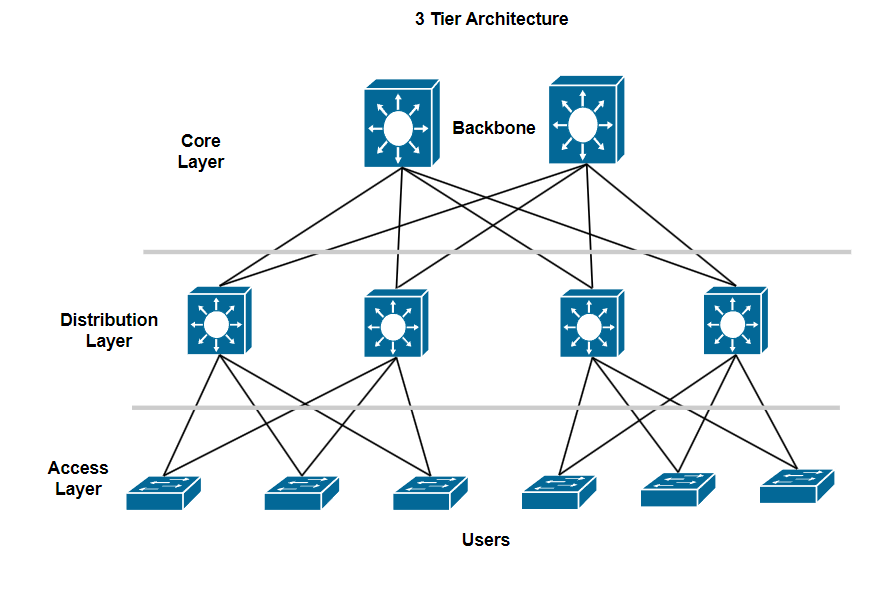
\includegraphics[width=0.80\textwidth]{image/mohinh.png}
    \caption{Mô hình mạng phân cấp Core--Distribution--Access}
    \label{fig:core_distribution_access}
\end{figure}

Tầng Access là tầng gần người dùng cuối nhất, nơi kết nối trực tiếp máy tính, điện thoại IP, camera, máy in, thiết bị Wi-Fi và các thiết bị đầu cuối khác. Tại tầng này, quản trị viên thường cấu hình cổng access, gán VLAN, áp dụng các chính sách bảo mật cơ bản, giới hạn truy cập và thu thập thông tin trạng thái kết nối. Vì tầng Access có số lượng cổng lớn nên tính dễ quản lý và khả năng chuẩn hóa cấu hình là yêu cầu quan trọng.

Tầng Distribution đóng vai trò tập trung lưu lượng từ nhiều switch Access, thực hiện định tuyến liên VLAN, áp dụng ACL, tổng hợp kết nối và triển khai các cơ chế dự phòng. Đây là tầng trung gian giúp kiểm soát chính sách giữa các vùng mạng khác nhau, ví dụ giữa VLAN sinh viên và VLAN máy chủ hoặc giữa VLAN khách và hệ thống nội bộ. Trong nhiều thiết kế Campus, tầng Distribution cũng là nơi đặt gateway mặc định cho các VLAN người dùng.

Tầng Core là xương sống của mạng Campus, chịu trách nhiệm chuyển tiếp lưu lượng tốc độ cao giữa các khu vực lớn trong hệ thống. Tầng Core cần được thiết kế đơn giản, ổn định và có khả năng dự phòng cao. Các thiết bị tại tầng này thường hạn chế xử lý chính sách phức tạp để ưu tiên tốc độ chuyển tiếp và độ tin cậy. Khi mạng có nhiều tòa nhà hoặc nhiều khu vực chức năng, tầng Core giúp kết nối các khối Distribution lại với nhau theo mô hình tập trung.

Việc áp dụng mô hình phân cấp giúp đề tài xây dựng được một topology rõ ràng: người dùng kết nối ở tầng Access, chính sách và định tuyến liên VLAN được xử lý ở tầng Distribution, còn tầng Core bảo đảm kết nối tốc độ cao giữa các vùng. Đây là nền tảng để triển khai thêm SDN Controller nhằm quản lý tập trung và SD-WAN nhằm kết nối nhiều cơ sở.

\subsection{VLAN và phân đoạn mạng}

\begin{figure}[H]
    \centering
    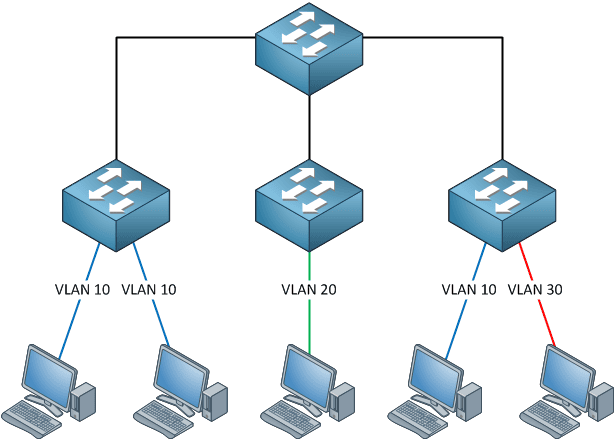
\includegraphics[width=0.80\textwidth]{image/vlan.png}
    \caption{Minh họa VLAN và phân đoạn mạng}
    \label{fig:vlan_phan_doan_mang}
\end{figure}

VLAN là kỹ thuật chia một hạ tầng switch vật lý thành nhiều mạng logic độc lập. Mỗi VLAN tương ứng với một miền quảng bá riêng, nhờ đó lưu lượng broadcast được giới hạn trong phạm vi cần thiết và các nhóm người dùng được tách biệt về mặt logic. Trong mạng Campus, VLAN thường được dùng để phân chia theo chức năng như VLAN sinh viên, VLAN giảng viên, VLAN hành chính, VLAN phòng máy, VLAN máy chủ, VLAN Wi-Fi khách và VLAN quản trị thiết bị.

Cổng access là cổng kết nối thiết bị đầu cuối và thường thuộc về một VLAN duy nhất. Ngược lại, cổng trunk được dùng để truyền lưu lượng của nhiều VLAN giữa các switch hoặc giữa switch và thiết bị định tuyến. Khi lưu lượng đi qua đường trunk, mỗi frame được gắn thẻ VLAN để thiết bị nhận biết frame đó thuộc mạng logic nào. Thiết kế trunk hợp lý giúp nhiều VLAN có thể cùng sử dụng một liên kết vật lý nhưng vẫn được phân tách về mặt logic.

Do các VLAN là các mạng khác nhau, thiết bị trong VLAN này muốn giao tiếp với VLAN khác cần có cơ chế định tuyến liên VLAN. Cơ chế này có thể được thực hiện bằng router, switch lớp 3 hoặc thiết bị gateway tại tầng Distribution. Trong đề tài, định tuyến liên VLAN là thành phần quan trọng để kiểm soát đường đi của lưu lượng giữa các khu vực chức năng. Ví dụ, VLAN sinh viên có thể được phép truy cập Internet và hệ thống học tập, nhưng không được truy cập trực tiếp VLAN quản trị thiết bị.

Phân đoạn mạng bằng VLAN không chỉ cải thiện hiệu năng mà còn tăng tính bảo mật. Khi kết hợp VLAN với ACL, NAC hoặc chính sách trên SDN Controller, hệ thống có thể kiểm soát quyền truy cập theo vai trò người dùng, vị trí kết nối hoặc loại dịch vụ. Đây là cơ sở để xây dựng chính sách mạng phù hợp với môi trường trường đại học có nhiều nhóm người dùng và mức độ tin cậy khác nhau.

\subsection{Định tuyến và dịch vụ mạng nền tảng}

\begin{figure}[H]
    \centering
    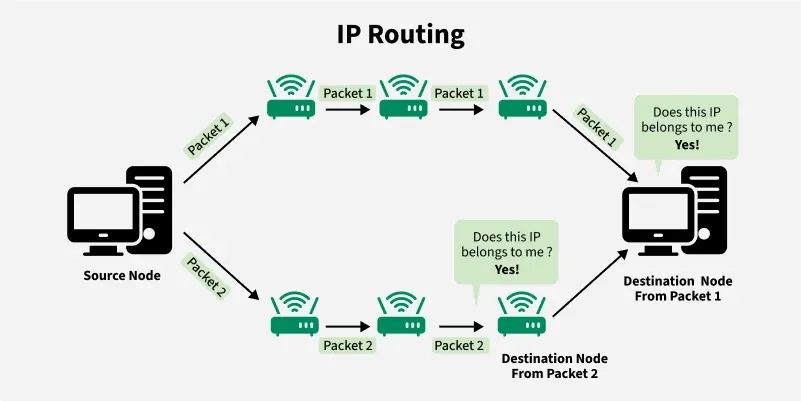
\includegraphics[width=0.80\textwidth]{image/iprouting.png}
    \caption{Minh họa định tuyến IP trong mạng}
    \label{fig:ip_routing}
\end{figure}

Định tuyến là quá trình xác định đường đi cho gói tin từ mạng nguồn đến mạng đích. Trong mạng Campus, định tuyến thường xuất hiện ở tầng Distribution hoặc Core để kết nối các VLAN, vùng máy chủ, vùng quản trị và đường ra Internet. Một thiết kế định tuyến tốt cần bảo đảm đường đi ổn định, dễ mở rộng và có khả năng hội tụ nhanh khi liên kết gặp sự cố.

OSPF là giao thức định tuyến nội bộ thường được dùng trong các hệ thống mạng có quy mô vừa và lớn. OSPF hoạt động theo cơ chế trạng thái liên kết, cho phép các router hoặc switch lớp 3 trao đổi thông tin topology và tự tính toán đường đi tối ưu. Ưu điểm của OSPF là hỗ trợ phân vùng, hội tụ tương đối nhanh và phù hợp với mô hình mạng phân cấp. Trong đề tài, OSPF có thể được sử dụng giữa các thiết bị Distribution và Core để tự động cập nhật đường đi thay vì cấu hình định tuyến tĩnh cho toàn bộ hệ thống.

DHCP là dịch vụ cấp phát địa chỉ IP tự động cho thiết bị đầu cuối. Trong môi trường Campus, DHCP giúp giảm khối lượng cấu hình thủ công, hạn chế trùng địa chỉ IP và hỗ trợ quản trị tập trung theo từng VLAN. Mỗi VLAN có thể được cấu hình một dải địa chỉ riêng, gateway mặc định, DNS và thời gian thuê địa chỉ phù hợp. Đối với các thiết bị hạ tầng như switch, router, server hoặc Controller, địa chỉ IP tĩnh vẫn nên được sử dụng để dễ quản lý và giám sát.

DNS là dịch vụ phân giải tên miền hoặc tên máy chủ thành địa chỉ IP. Trong mạng nội bộ, DNS giúp người dùng truy cập dịch vụ bằng tên dễ nhớ thay vì địa chỉ IP. Ngoài DNS, hệ thống Campus còn cần các dịch vụ nền tảng khác như NTP để đồng bộ thời gian, Syslog để ghi nhận sự kiện, SNMP hoặc giao thức giám sát tương đương để theo dõi trạng thái thiết bị. Các dịch vụ này hỗ trợ đáng kể cho vận hành, kiểm thử và đánh giá hệ thống.

\subsection{Cơ chế bảo mật và dự phòng trong mạng Campus}

Bảo mật mạng Campus cần được triển khai theo nhiều lớp, từ phân đoạn mạng, kiểm soát truy cập, bảo vệ cổng kết nối đến giám sát lưu lượng. ACL là một cơ chế phổ biến dùng để cho phép hoặc từ chối lưu lượng dựa trên địa chỉ nguồn, địa chỉ đích, giao thức và cổng dịch vụ. Khi đặt ACL tại tầng Distribution hoặc gateway liên VLAN, quản trị viên có thể kiểm soát chặt chẽ luồng dữ liệu giữa các nhóm người dùng.

Một nguyên tắc quan trọng là chỉ cho phép những truy cập cần thiết cho mục tiêu nghiệp vụ. Ví dụ, VLAN sinh viên có thể truy cập máy chủ học tập và Internet nhưng không được truy cập vùng quản trị; VLAN khách chỉ được truy cập Internet; VLAN quản trị được phép truy cập giao diện quản lý thiết bị; còn VLAN máy chủ chỉ mở các dịch vụ cần thiết. Cách tiếp cận này giúp giảm bề mặt tấn công và hạn chế lan truyền sự cố trong mạng nội bộ.

Ở tầng Access, các kỹ thuật như giới hạn địa chỉ MAC, tắt cổng không sử dụng, cấu hình VLAN riêng cho khách và kiểm soát truy cập theo người dùng giúp tăng mức an toàn cho điểm kết nối đầu cuối. Với hệ thống Wi-Fi, việc tách SSID theo nhóm người dùng và ánh xạ từng SSID vào VLAN phù hợp giúp chính sách truy cập nhất quán giữa mạng có dây và không dây.

Dự phòng là yêu cầu không thể thiếu trong mạng Campus vì sự cố tại một liên kết hoặc thiết bị có thể ảnh hưởng đến nhiều người dùng. STP hoặc RSTP được sử dụng để ngăn vòng lặp lớp 2 khi tồn tại nhiều đường kết nối dự phòng giữa các switch. Ở lớp 3, OSPF có thể tự động chọn đường thay thế khi một liên kết bị lỗi. Ngoài ra, thiết kế có thể sử dụng liên kết kép, thiết bị Core/Distribution dự phòng và nguồn điện dự phòng để tăng tính sẵn sàng của hệ thống.

\subsection{Công nghệ SDN}

SDN (Software-Defined Networking) là mô hình mạng dựa trên phần mềm, trong đó mặt phẳng điều khiển (control plane) được tách khỏi mặt phẳng chuyển tiếp dữ liệu (data plane). Trong mạng truyền thống, mỗi router hoặc switch thường tự đảm nhiệm cả việc tính toán đường đi, lưu giữ bảng định tuyến và chuyển tiếp gói tin. Với SDN, các quyết định điều khiển được tập trung tại bộ điều khiển SDN Controller, còn thiết bị mạng ở phía dưới chủ yếu thực hiện chuyển tiếp theo các quy tắc hoặc luồng dữ liệu do Controller cung cấp.

Cách tiếp cận này giúp trừu tượng hóa hạ tầng mạng và làm cho quá trình quản trị trở nên linh hoạt hơn. Quản trị viên có thể giám sát topology, điều chỉnh chính sách lưu lượng, thay đổi đường đi hoặc triển khai dịch vụ mạng từ một điểm quản lý tập trung thay vì cấu hình thủ công trên từng thiết bị riêng lẻ. Nhờ đó, SDN phù hợp với các hệ thống cần mở rộng nhanh, thay đổi chính sách thường xuyên và yêu cầu khả năng tự động hóa cao như trung tâm dữ liệu, điện toán đám mây, mạng doanh nghiệp và mạng Campus.

\subsubsection{Kiến trúc SDN ba lớp}

Kiến trúc SDN thường được mô tả theo ba lớp chính: lớp ứng dụng, lớp điều khiển và lớp hạ tầng. Ba lớp này phối hợp với nhau thông qua các giao diện lập trình để triển khai chính sách mạng một cách tập trung và nhất quán.

\begin{figure}[H]
    \centering
    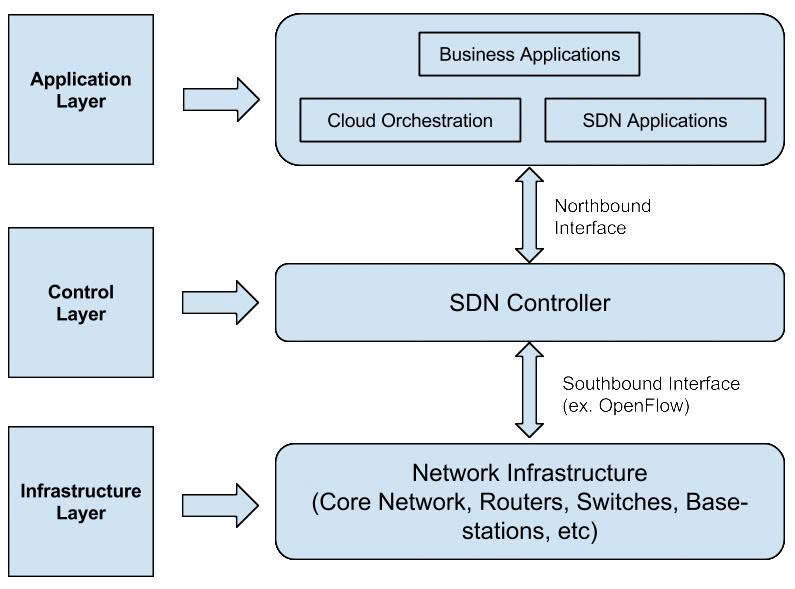
\includegraphics[width=0.60\textwidth]{image/SDN_ARCHITECTURE.jpg}
    \caption{Kiến trúc tổng quan của SDN}
    \label{fig:sdn_architecture}
\end{figure}

Lớp ứng dụng (Application Layer) là nơi triển khai các ứng dụng và dịch vụ mạng như giám sát, bảo mật, cân bằng tải, quản lý QoS, tối ưu băng thông hoặc tự động hóa cấu hình. Các ứng dụng này không trực tiếp cấu hình thiết bị mạng mà gửi yêu cầu đến SDN Controller thông qua giao diện northbound API. Nhờ đó, yêu cầu nghiệp vụ có thể được chuyển thành chính sách mạng cụ thể.

Lớp điều khiển (Control Layer) là thành phần trung tâm của SDN, thường được gọi là SDN Controller. Controller đóng vai trò như ``bộ não'' của mạng vì có khả năng thu thập thông tin topology, trạng thái liên kết, bảng luồng và chính sách vận hành. Dựa trên thông tin toàn cục này, Controller ra quyết định về định tuyến, phân bổ tài nguyên, kiểm soát truy cập hoặc chất lượng dịch vụ. Sau đó, Controller gửi chỉ thị xuống các thiết bị mạng thông qua giao diện southbound.

Lớp hạ tầng hoặc mặt phẳng dữ liệu (Infrastructure Layer/Data Plane) bao gồm các switch, router, firewall hoặc thiết bị mạng ảo. Nhiệm vụ chính của lớp này là chuyển tiếp gói tin theo các quy tắc đã được cài đặt trong bảng luồng. Các thiết bị ở lớp hạ tầng không cần tự xử lý toàn bộ logic điều khiển phức tạp mà tập trung vào việc thực thi nhanh và chính xác các quyết định do Controller đưa xuống.

\subsubsection{Nguyên lý hoạt động của SDN}

SDN hoạt động dựa trên cơ chế tách biệt giữa control plane và data plane. Khi một gói tin đi vào switch, thiết bị sẽ kiểm tra bảng luồng (flow table) để xác định cách xử lý. Nếu đã có quy tắc phù hợp, gói tin được chuyển tiếp, loại bỏ hoặc xử lý theo hành động đã định nghĩa. Nếu chưa có quy tắc, switch có thể gửi thông tin về gói tin hoặc luồng mới lên SDN Controller để xin quyết định xử lý.

\begin{figure}[H]
    \centering
    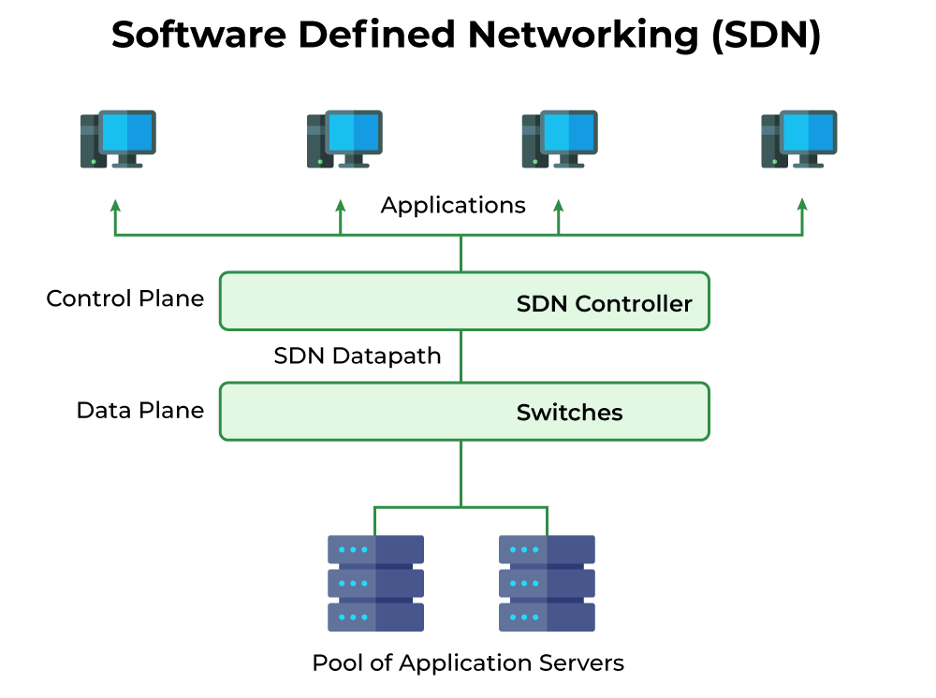
\includegraphics[width=0.80\textwidth]{image/nguyenlyhoatdongsdn.png}
    \caption{Nguyên lý hoạt động của SDN}
    \label{fig:nguyen_ly_hoat_dong_sdn}
\end{figure}

Sau khi nhận yêu cầu, Controller phân tích thông tin gói tin, trạng thái mạng và chính sách đang áp dụng. Controller có thể quyết định đường đi tối ưu, áp dụng chính sách bảo mật, giới hạn băng thông hoặc ưu tiên một loại lưu lượng nhất định. Quyết định này được chuyển lại cho switch dưới dạng quy tắc mới. Từ thời điểm đó, các gói tin cùng loại có thể được xử lý trực tiếp tại switch mà không cần hỏi Controller lặp lại, giúp giảm độ trễ và tăng hiệu quả chuyển tiếp.

Trong môi trường Campus, nguyên lý này cho phép hệ thống thay đổi chính sách theo trạng thái mạng hoặc theo nhóm người dùng. Ví dụ, Controller có thể ưu tiên lưu lượng học trực tuyến, giới hạn lưu lượng từ VLAN khách, cô lập một thiết bị có dấu hiệu bất thường hoặc điều chỉnh đường đi khi một liên kết bị nghẽn. Điều này giúp mạng phản ứng linh hoạt hơn so với mô hình cấu hình tĩnh truyền thống.

\subsubsection{Các giao thức và giao diện trong SDN}

OpenFlow là giao thức southbound phổ biến trong các mô hình SDN, cho phép Controller cài đặt, sửa đổi hoặc xóa các quy tắc trong bảng luồng của switch. Thông qua OpenFlow, Controller có thể quy định cách thiết bị xử lý gói tin dựa trên địa chỉ MAC, địa chỉ IP, cổng TCP/UDP, VLAN ID hoặc các trường tiêu đề khác. Đây là nền tảng quan trọng để SDN điều khiển lưu lượng ở mức chi tiết.

Bên cạnh OpenFlow, SDN còn có thể sử dụng nhiều cơ chế giao tiếp khác tùy theo thiết bị và nền tảng triển khai. Một số hệ thống dùng REST API, NETCONF, gRPC, SNMP hoặc giao diện dòng lệnh được tự động hóa để quản lý thiết bị mạng. Ở chiều ngược lại, northbound API giúp các ứng dụng quản trị, giám sát, bảo mật hoặc tự động hóa gửi yêu cầu chính sách đến Controller. Nhờ các giao diện này, SDN có thể tích hợp với hệ thống quản lý mạng, nền tảng giám sát, công cụ DevOps hoặc các dịch vụ đám mây.

Đối với đề tài, các giao thức và giao diện trong SDN có ý nghĩa quan trọng vì chúng là cầu nối giữa chính sách quản trị tập trung và thiết bị mạng Campus. Controller có thể thu thập trạng thái mạng, nhận biết liên kết, quản lý luồng dữ liệu và triển khai chính sách cho từng VLAN hoặc từng nhóm dịch vụ mà không cần cấu hình thủ công trên toàn bộ thiết bị.

\subsubsection{Phân loại mô hình SDN}

SDN có thể được triển khai theo nhiều mô hình khác nhau. Open SDN là mô hình sử dụng giao thức mở như OpenFlow để Controller điều khiển trực tiếp hành vi chuyển tiếp của switch. Mô hình này phù hợp với môi trường nghiên cứu, thử nghiệm hoặc các hệ thống cần kiểm soát chi tiết luồng dữ liệu.

SDN thông qua API là mô hình tận dụng các giao diện lập trình do thiết bị mạng cung cấp. Thay vì thay đổi hoàn toàn cơ chế chuyển tiếp của thiết bị, Controller hoặc hệ thống quản lý sử dụng API như REST API, NETCONF hoặc các công cụ tự động hóa để cấu hình thiết bị từ xa. Mô hình này phù hợp với môi trường có nhiều thiết bị sẵn có và cần chuyển đổi từng bước sang quản lý tập trung.

SDN dựa trên hypervisor tập trung vào ảo hóa mạng trong trung tâm dữ liệu hoặc môi trường cloud. Các mạng ảo, switch ảo và chính sách kết nối giữa máy ảo được tạo và quản lý trên lớp ảo hóa mà không cần thay đổi quá nhiều hạ tầng vật lý. Ngoài ra, mô hình Hybrid SDN kết hợp mạng truyền thống với SDN, trong đó một phần thiết bị vẫn vận hành theo cơ chế cũ, còn một phần được điều khiển bởi Controller. Đây là hướng phù hợp cho tổ chức muốn tận dụng hạ tầng hiện có và giảm chi phí chuyển đổi ban đầu.

\subsubsection{Ưu và nhược điểm của SDN}

Ưu điểm lớn nhất của SDN là khả năng quản lý tập trung. Controller cung cấp một điểm điều khiển chung cho toàn mạng, giúp giảm sai sót khi cấu hình thủ công và hỗ trợ triển khai chính sách nhất quán. SDN cũng tăng tính linh hoạt vì quản trị viên có thể thay đổi đường đi, cập nhật ACL, điều chỉnh QoS hoặc bổ sung dịch vụ mới thông qua phần mềm.

SDN còn hỗ trợ tối ưu hóa tài nguyên và hiệu năng mạng. Nhờ có cái nhìn tổng thể về topology và trạng thái liên kết, Controller có thể lựa chọn đường đi phù hợp, phân bổ băng thông hiệu quả hơn và giảm tình trạng nghẽn mạng. Khả năng tự động hóa cũng giúp rút ngắn thời gian triển khai dịch vụ, hỗ trợ mở rộng hệ thống và tích hợp với các công nghệ hiện đại như điện toán đám mây, NFV, IoT hoặc SD-WAN.

Tuy nhiên, SDN cũng tồn tại một số hạn chế. Controller là thành phần trung tâm nên nếu không được bảo vệ và dự phòng tốt, nó có thể trở thành điểm lỗi hoặc mục tiêu tấn công quan trọng. Việc triển khai SDN cũng đòi hỏi nhân sự có kiến thức về mạng, lập trình, API và bảo mật. Ngoài ra, sự khác biệt giữa các nhà cung cấp thiết bị có thể gây khó khăn khi tích hợp trong môi trường đa hãng. Chi phí đầu tư ban đầu cho Controller, thiết bị tương thích và đào tạo cũng là yếu tố cần cân nhắc.

\subsubsection{Ứng dụng thực tế của SDN}

SDN được ứng dụng rộng rãi trong trung tâm dữ liệu để quản lý lưu lượng quy mô lớn, tự động hóa cấu hình mạng ảo và triển khai chính sách bảo mật nhanh chóng. Trong mạng đám mây, SDN hỗ trợ tạo mạng ảo cho nhiều người thuê, cô lập tài nguyên và mở rộng dịch vụ linh hoạt. Trong mạng doanh nghiệp, SDN giúp đơn giản hóa quản trị. 

Đối với mạng Campus, SDN có thể được sử dụng để quản lý tập trung các VLAN, áp dụng chính sách truy cập theo nhóm người dùng, giám sát trạng thái liên kết, ưu tiên lưu lượng quan trọng và hỗ trợ phát hiện bất thường. Trong phạm vi đề tài, SDN không thay thế hoàn toàn mô hình Core--Distribution--Access mà đóng vai trò là lớp điều phối và quản lý tập trung. Hạ tầng phân cấp vẫn đảm nhiệm tổ chức vật lý và logic của mạng, trong khi SDN Controller giúp triển khai chính sách nhất quán, giảm cấu hình thủ công và hỗ trợ vận hành mạng Campus hiệu quả hơn.

\subsection{Công nghệ SD-WAN}

\begin{figure}[H]
    \centering
    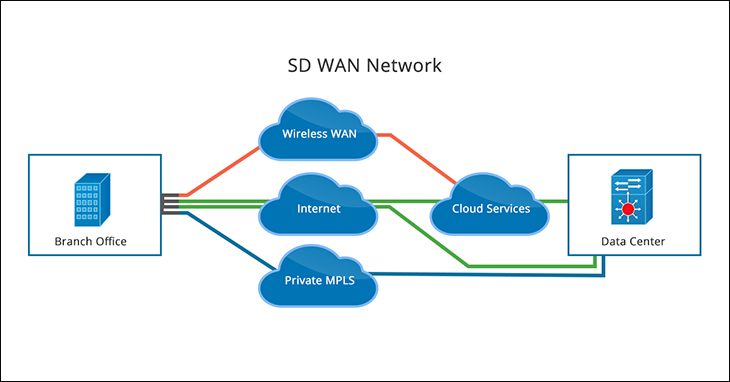
\includegraphics[width=0.80\textwidth]{image/sdwan.jpg}
    \caption{Minh họa công nghệ SD-WAN}
    \label{fig:sdwan}
\end{figure}

SD-WAN là công nghệ mạng diện rộng được điều khiển bằng phần mềm, cho phép quản lý tập trung các kết nối WAN giữa nhiều địa điểm. Thay vì phụ thuộc hoàn toàn vào một đường truyền riêng, SD-WAN có thể kết hợp nhiều loại kết nối như Internet, leased line hoặc 4G/5G và lựa chọn đường truyền phù hợp dựa trên chính sách, chất lượng đường truyền.

Trong môi trường trường đại học có nhiều cơ sở, SD-WAN giúp kết nối Campus chính với các cơ sở phụ, trung tâm dữ liệu hoặc dịch vụ đám mây một cách linh hoạt hơn. Hệ thống có thể ưu tiên lưu lượng quan trọng như hệ thống quản lý đào tạo, họp trực tuyến hoặc truy cập máy chủ nội bộ qua đường truyền có độ trễ thấp; trong khi lưu lượng thông thường có thể đi qua đường Internet chi phí thấp hơn. Khi một đường truyền gặp sự cố, SD-WAN có thể chuyển lưu lượng sang đường thay thế để duy trì kết nối.

Một thành phần quan trọng của SD-WAN là chính sách điều hướng lưu lượng theo ứng dụng. Chính sách này có thể dựa trên độ trễ, jitter, tỷ lệ mất gói, băng thông còn lại hoặc yêu cầu SLA. Nhờ đó, hệ thống không chỉ dự phòng ở mức kết nối mà còn tối ưu trải nghiệm người dùng. Bên cạnh đó, SD-WAN thường hỗ trợ mã hóa đường truyền, quản lý tập trung và hiển thị trạng thái kết nối giữa các site.

Trong phạm vi đề tài, SD-WAN được định hướng sử dụng cho bài toán kết nối nhiều cơ sở đào tạo. Mạng Campus tại cơ sở chính cung cấp các dịch vụ dùng chung, còn cơ sở phụ cần truy cập ổn định và an toàn đến các dịch vụ này. Khi kết hợp với SDN, SD-WAN giúp mở rộng quản trị từ mạng nội bộ ra WAN.

	\newpage

    \section{MÔ HÌNH MẠNG CAMPUS ĐỀ XUẤT}\label{sec:mo_hinh_de_xuat}

\subsection{Phân tích bài toán và yêu cầu thiết kế hệ thống}

Hệ thống mạng Campus được thiết kế nhằm phục vụ đồng thời nhiều nhóm người dùng và nhiều khu vực chức năng trong trường đại học, bao gồm khoa chuyên môn, phòng học lý thuyết, phòng máy thực hành, khu vực hành chính, thư viện, hệ thống máy chủ nội bộ, mạng không dây và các cơ sở phụ. Do đó, mô hình mạng cần đáp ứng các yêu cầu về khả năng kết nối ổn định, phân tách lưu lượng hợp lý, dễ quản trị, bảo mật và có khả năng mở rộng khi quy mô đào tạo tăng lên.

Trước hết, hệ thống phải bảo đảm kết nối nội bộ giữa các khu vực trong Campus chính. Các khoa, phòng ban và phòng học cần truy cập được các dịch vụ dùng chung như hệ thống quản lý đào tạo, máy chủ xác thực, máy chủ tập tin, hệ thống học trực tuyến và Internet. Đối với phòng máy thực hành, mạng cần hỗ trợ số lượng thiết bị lớn, băng thông ổn định và khả năng cấp phát địa chỉ IP tự động để thuận tiện cho việc tổ chức lớp học, thực hành mạng hoặc triển khai phần mềm theo từng học phần.

Đối với khu vực hành chính, yêu cầu quan trọng là bảo mật và kiểm soát truy cập. Các máy trạm thuộc phòng đào tạo, kế toán, nhân sự hoặc ban quản lý cần được tách riêng khỏi mạng sinh viên và mạng khách. Việc phân tách này giúp hạn chế truy cập trái phép, giảm nguy cơ lây lan sự cố giữa các khu vực và tạo điều kiện áp dụng các chính sách truy cập khác nhau theo vai trò người dùng.

Khu vực máy chủ nội bộ cần được thiết kế như một vùng dịch vụ riêng, có địa chỉ IP tĩnh, dễ giám sát và được bảo vệ bằng các chính sách truy cập chặt chẽ. Chỉ những VLAN hoặc nhóm người dùng có nhu cầu hợp lệ mới được phép truy cập các dịch vụ tương ứng. Ngoài ra, vùng máy chủ cần có kết nối tốc độ cao đến tầng Core hoặc Distribution để bảo đảm hiệu năng cho các dịch vụ quan trọng của nhà trường.

Mạng Wi-Fi cần hỗ trợ nhiều nhóm truy cập khác nhau như giảng viên, sinh viên, khách và thiết bị di động. Mỗi nhóm truy cập không dây nên được ánh xạ vào VLAN riêng để có chính sách cấp phát địa chỉ, giới hạn băng thông và kiểm soát truy cập phù hợp. Đối với mạng khách, hệ thống chỉ nên cho phép truy cập Internet và hạn chế truy cập vào tài nguyên nội bộ của trường.

Bên cạnh Campus chính, mô hình cũng cần hỗ trợ kết nối đến các cơ sở phụ hoặc chi nhánh đào tạo. Các cơ sở này cần truy cập được một số dịch vụ tập trung đặt tại Campus chính, đồng thời vẫn duy trì được kết nối Internet cục bộ. Vì vậy, thiết kế cần có cơ chế SD-WAN để quản lý nhiều đường truyền WAN, lựa chọn đường đi phù hợp, tự động chuyển hướng khi đường truyền gặp sự cố và tối ưu lưu lượng giữa các site.

Về mặt vận hành, hệ thống phải giảm phụ thuộc vào cấu hình thủ công trên từng thiết bị. SDN Controller được sử dụng để quản lý tập trung các switch, triển khai chính sách mạng, theo dõi trạng thái luồng dữ liệu và hỗ trợ thay đổi cấu hình nhanh hơn khi bổ sung VLAN, thêm khu vực mới hoặc điều chỉnh chính sách truy cập. Yêu cầu này giúp nâng cao tính nhất quán trong cấu hình và giảm sai sót trong quá trình quản trị.

\subsubsection{Bài toán đơn giản hóa quá trình quản lý mạng Campus}

Trong mô hình mạng Campus truyền thống, quá trình quản lý thường phụ thuộc nhiều vào việc cấu hình thủ công trên từng thiết bị như switch, router, thiết bị tường lửa và bộ điều khiển Wi-Fi. Khi quy mô mạng còn nhỏ, cách quản trị này có thể đáp ứng được các nhu cầu cơ bản. Tuy nhiên, khi số lượng VLAN, phòng học, phòng máy, điểm truy cập không dây, máy chủ và cơ sở phụ tăng lên, việc cấu hình riêng lẻ trên từng thiết bị trở nên phức tạp, tốn thời gian và dễ phát sinh sai sót.

Một thay đổi nhỏ trong chính sách mạng, chẳng hạn bổ sung VLAN cho một khoa mới, thay đổi quyền truy cập của mạng sinh viên hoặc cập nhật ACL cho vùng máy chủ, có thể yêu cầu quản trị viên thao tác trên nhiều thiết bị khác nhau. Nếu các cấu hình này không được triển khai đồng bộ, hệ thống có thể xảy ra lỗi định tuyến, sai lệch chính sách truy cập, trùng lặp địa chỉ IP hoặc gián đoạn dịch vụ. Đây là vấn đề đặc biệt quan trọng đối với môi trường đại học, nơi mạng phải phục vụ liên tục cho hoạt động giảng dạy, học tập, nghiên cứu và quản lý hành chính.

Do đó, bài toán đặt ra là cần đơn giản hóa quá trình quản lý mạng Campus theo hướng tập trung, nhất quán và dễ mở rộng. Thay vì quản trị từng thiết bị riêng lẻ, hệ thống cần cho phép cấu hình, giám sát và áp dụng chính sách từ một điểm quản lý trung tâm. Cách tiếp cận này giúp quản trị viên dễ dàng theo dõi trạng thái mạng, kiểm soát lưu lượng giữa các VLAN, triển khai chính sách bảo mật theo nhóm người dùng và nhanh chóng điều chỉnh cấu hình khi có thay đổi về tổ chức hoặc hạ tầng.

Việc ứng dụng SDN Controller và SD-WAN trong mô hình đề xuất nhằm giải quyết trực tiếp bài toán trên. SDN Controller hỗ trợ quản lý tập trung hạ tầng mạng nội bộ trong Campus, trong khi SD-WAN giúp đơn giản hóa việc điều phối kết nối giữa Campus chính và các cơ sở phụ. Nhờ đó, hệ thống mạng không chỉ giảm khối lượng cấu hình thủ công mà còn nâng cao khả năng giám sát, phát hiện sự cố, chuẩn hóa chính sách và mở rộng mạng trong tương lai.

\subsubsection{Cơ sở lựa chọn mô hình đề xuất}

Mô hình mạng Campus đề xuất được lựa chọn dựa trên đặc điểm tổ chức của môi trường đại học, nhu cầu vận hành thực tế và xu hướng quản trị mạng hiện đại. Trong môi trường này, hệ thống mạng không chỉ phục vụ một nhóm người dùng cố định mà phải đáp ứng đồng thời nhiều đối tượng như cán bộ quản lý, giảng viên, sinh viên, khách truy cập, thiết bị phòng máy, máy chủ nội bộ và các cơ sở phụ. Vì vậy, một mô hình mạng đơn giản, ít phân lớp hoặc thiếu khả năng quản lý tập trung sẽ khó đáp ứng yêu cầu về hiệu năng, bảo mật và mở rộng lâu dài.

Cơ sở đầu tiên của mô hình đề xuất là kiến trúc phân lớp Core--Distribution--Access. Kiến trúc này giúp tách rõ vai trò của từng tầng mạng: tầng Access kết nối trực tiếp thiết bị đầu cuối, tầng Distribution thực hiện tập trung lưu lượng và áp dụng chính sách, còn tầng Core đảm nhiệm chuyển mạch tốc độ cao giữa các khu vực chính. Cách tổ chức này phù hợp với mạng Campus vì dễ mở rộng khi bổ sung thêm phòng học, khoa, tòa nhà hoặc thiết bị mạng mới mà không làm thay đổi toàn bộ cấu trúc hệ thống.

Cơ sở thứ hai là nhu cầu phân tách lưu lượng theo khu vực chức năng. Việc sử dụng VLAN cho từng nhóm người dùng và từng vùng dịch vụ giúp giảm miền quảng bá, nâng cao khả năng kiểm soát truy cập và hạn chế ảnh hưởng khi xảy ra sự cố. Đối với trường đại học, đây là yêu cầu quan trọng vì mạng sinh viên, mạng hành chính, mạng giảng viên, mạng khách và vùng máy chủ có mức độ tin cậy cũng như quyền truy cập khác nhau. Khi kết hợp VLAN với định tuyến liên VLAN và ACL, hệ thống có thể kiểm soát luồng truy cập một cách rõ ràng hơn.

Cơ sở thứ ba là yêu cầu quản trị tập trung. SDN Controller được đưa vào mô hình nhằm giảm phụ thuộc vào cấu hình thủ công trên từng thiết bị, đồng thời hỗ trợ giám sát trạng thái mạng, triển khai chính sách đồng nhất và thay đổi cấu hình nhanh hơn. Điều này đặc biệt cần thiết trong bối cảnh mạng Campus thường xuyên có thay đổi về người dùng, lớp học, phòng máy, thiết bị Wi-Fi hoặc chính sách truy cập theo từng học kỳ.

Cơ sở thứ tư là nhu cầu kết nối nhiều cơ sở đào tạo. SD-WAN được lựa chọn để hỗ trợ điều phối các đường truyền WAN giữa Campus chính và cơ sở phụ, tối ưu lưu lượng truy cập đến dịch vụ tập trung, đồng thời nâng cao khả năng dự phòng khi một đường truyền gặp sự cố. So với cách kết nối WAN truyền thống, SD-WAN phù hợp hơn với yêu cầu quản lý linh hoạt, theo dõi chất lượng đường truyền và lựa chọn tuyến dựa trên chính sách.

Như vậy, mô hình đề xuất là sự kết hợp giữa kiến trúc mạng Campus phân lớp, phân hoạch VLAN, quản lý tập trung bằng SDN Controller và kết nối liên cơ sở bằng SD-WAN. Sự kết hợp này giúp hệ thống đạt được các mục tiêu chính gồm ổn định, dễ quản trị, bảo mật, linh hoạt và có khả năng mở rộng trong tương lai.

\subsubsection{Phạm vi giả định của hệ thống}

Để thuận lợi cho quá trình thiết kế, mô hình mạng Campus trong đề tài được xây dựng trên một số giả định nhất định. Các giả định này nhằm giới hạn phạm vi nghiên cứu, giúp việc quy hoạch topology, VLAN, địa chỉ IP, chính sách truy cập và kết nối WAN được trình bày rõ ràng, có tính hệ thống và phù hợp với mục tiêu của đề tài.

Thứ nhất, hệ thống giả định có một Campus chính đóng vai trò trung tâm và một hoặc nhiều cơ sở phụ kết nối về Campus chính thông qua hạ tầng WAN. Campus chính bao gồm các khu vực chức năng cơ bản như khu hành chính, các khoa chuyên môn, phòng học lý thuyết, phòng máy thực hành, thư viện, vùng máy chủ nội bộ, hệ thống Wi-Fi và khu vực quản trị thiết bị mạng. Các cơ sở phụ có quy mô nhỏ hơn, chủ yếu cần truy cập Internet cục bộ và một số dịch vụ dùng chung đặt tại Campus chính.

Thứ hai, mô hình tập trung vào thiết kế logic và kiến trúc kết nối ở mức tổng thể, chưa đi sâu vào lựa chọn chính xác chủng loại thiết bị, số lượng cổng vật lý, cấu hình chi tiết từng dòng lệnh hoặc chi phí triển khai thực tế. Các thiết bị như switch Core, switch Distribution, switch Access, router biên, firewall, SDN Controller và thiết bị SD-WAN được xem là các thành phần chức năng trong mô hình nhằm mô tả vai trò và quan hệ kết nối giữa chúng.

Thứ ba, hệ thống sử dụng địa chỉ IPv4 private cho các VLAN nội bộ. Mỗi khu vực chức năng được cấp một subnet riêng để thuận tiện cho quản lý, định tuyến và áp dụng chính sách bảo mật. Việc cấp phát địa chỉ IP cho người dùng cuối được giả định thực hiện thông qua DHCP, trong khi các thiết bị hạ tầng mạng, máy chủ và gateway VLAN sử dụng địa chỉ IP tĩnh để bảo đảm tính ổn định khi vận hành.

Thứ tư, các dịch vụ nội bộ được giả định đặt tại vùng máy chủ của Campus chính, bao gồm máy chủ xác thực, máy chủ tập tin, hệ thống học trực tuyến, hệ thống quản lý đào tạo và một số dịch vụ quản trị mạng. Người dùng tại các VLAN khác nhau chỉ được truy cập những dịch vụ phù hợp với vai trò của mình. Mạng khách được giả định chỉ có quyền truy cập Internet và không được truy cập trực tiếp vào tài nguyên nội bộ.

Thứ năm, phạm vi bảo mật của đề tài tập trung vào các chính sách ở mức mạng như phân tách VLAN, ACL, kiểm soát truy cập giữa các vùng, vùng quản trị thiết bị và nguyên tắc cô lập mạng khách. Các nội dung bảo mật chuyên sâu như mã hóa ứng dụng, bảo mật cơ sở dữ liệu, kiểm thử xâm nhập hoặc triển khai hệ thống phát hiện xâm nhập chi tiết không thuộc phạm vi chính của phần thiết kế này.

Với các giả định trên, mô hình đề xuất có thể đại diện cho một hệ thống mạng Campus ở mức vừa và có khả năng mở rộng. Phạm vi này đủ để thể hiện vai trò của kiến trúc phân lớp, SDN Controller, SD-WAN, VLAN, định tuyến nội bộ và chính sách bảo mật trong việc xây dựng một hệ thống mạng đại học có tính quản trị tập trung và vận hành ổn định.

\subsubsection{Yêu cầu chức năng và phi chức năng của hệ thống}

Từ bài toán thiết kế và phạm vi giả định đã nêu, hệ thống mạng Campus cần đáp ứng hai nhóm yêu cầu chính: yêu cầu chức năng và yêu cầu phi chức năng. Yêu cầu chức năng mô tả những nhiệm vụ mà hệ thống phải thực hiện, trong khi yêu cầu phi chức năng phản ánh chất lượng vận hành, mức độ ổn định, bảo mật, khả năng mở rộng và khả năng quản trị của hệ thống.

Về yêu cầu chức năng, hệ thống trước hết phải cung cấp kết nối mạng cho toàn bộ các khu vực trong Campus chính và các cơ sở phụ. Người dùng thuộc các khoa, phòng học, phòng máy, khu hành chính, thư viện và mạng Wi-Fi cần truy cập được Internet cũng như các dịch vụ nội bộ được phép sử dụng. Các cơ sở phụ cần có khả năng kết nối về Campus chính để khai thác dịch vụ tập trung, đồng thời vẫn duy trì truy cập Internet tại chỗ.

Hệ thống phải hỗ trợ phân tách mạng bằng VLAN theo từng khu vực chức năng và nhóm người dùng. Mỗi VLAN cần có subnet, gateway và chính sách truy cập riêng. Việc định tuyến giữa các VLAN được thực hiện tại tầng Core hoặc Distribution, nhưng không phải mọi VLAN đều được phép truy cập lẫn nhau. Các luồng truy cập phải được kiểm soát bằng ACL hoặc chính sách tương đương nhằm bảo đảm nguyên tắc chỉ cho phép những kết nối cần thiết.

Hệ thống cũng cần cung cấp dịch vụ cấp phát địa chỉ IP động cho các mạng người dùng, phòng máy và Wi-Fi thông qua DHCP. Đối với vùng máy chủ, thiết bị mạng, thiết bị quản trị và các gateway quan trọng, hệ thống phải hỗ trợ sử dụng địa chỉ IP tĩnh để thuận tiện cho giám sát, ghi nhận nhật ký và xử lý sự cố. Bên cạnh đó, hệ thống cần có cơ chế truy cập đến các dịch vụ dùng chung như xác thực, lưu trữ tập tin, học trực tuyến và quản lý đào tạo.

Một yêu cầu chức năng quan trọng khác là quản lý tập trung. SDN Controller cần hỗ trợ quản trị viên theo dõi trạng thái thiết bị, giám sát luồng dữ liệu, triển khai cấu hình hoặc chính sách mạng từ một điểm điều khiển trung tâm. Đối với kết nối liên cơ sở, SD-WAN cần hỗ trợ lựa chọn đường truyền, tự động chuyển hướng khi có sự cố và ưu tiên lưu lượng quan trọng theo chính sách đã định.

Về yêu cầu phi chức năng, hệ thống phải bảo đảm tính sẵn sàng và ổn định trong quá trình vận hành. Các thành phần quan trọng như tầng Core, Distribution, kết nối WAN và vùng máy chủ cần được thiết kế theo hướng có dự phòng phù hợp để hạn chế gián đoạn dịch vụ. Khi một đường truyền hoặc một thiết bị trung gian gặp sự cố, hệ thống cần có khả năng duy trì kết nối ở mức chấp nhận được hoặc nhanh chóng khôi phục hoạt động.

Hệ thống phải có khả năng mở rộng khi số lượng người dùng, phòng máy, thiết bị Wi-Fi, máy chủ hoặc cơ sở đào tạo tăng lên. Việc mở rộng cần được thực hiện bằng cách bổ sung VLAN, subnet, switch Access hoặc đường truyền WAN mà không làm thay đổi lớn đến kiến trúc tổng thể. Đây là yêu cầu quan trọng để bảo đảm mô hình có thể đáp ứng sự phát triển của nhà trường trong nhiều giai đoạn.

Về bảo mật, hệ thống phải bảo đảm phân quyền truy cập theo vai trò người dùng và khu vực chức năng. Mạng hành chính, mạng máy chủ và mạng quản trị thiết bị cần được bảo vệ chặt chẽ hơn so với mạng sinh viên hoặc mạng khách. Các chính sách bảo mật phải hướng đến việc giảm truy cập trái phép, hạn chế lan truyền sự cố và hỗ trợ quản trị viên kiểm soát tốt hơn các luồng dữ liệu trong mạng.

Ngoài ra, hệ thống cần có tính dễ quản trị và dễ giám sát. Cấu trúc địa chỉ IP, tên VLAN, sơ đồ kết nối và chính sách truy cập phải được tổ chức rõ ràng để thuận tiện cho vận hành lâu dài. Khi có thay đổi về tổ chức, lớp học, phòng ban hoặc dịch vụ, quản trị viên cần có thể điều chỉnh cấu hình một cách nhanh chóng, nhất quán và ít gây gián đoạn đến hoạt động chung của hệ thống.

Từ các yêu cầu trên, hệ thống mạng đề xuất cần thỏa mãn các tiêu chí chính sau:

\begin{itemize}
    \item Bảo đảm kết nối ổn định cho các khoa, phòng học, phòng máy, khu hành chính, vùng máy chủ, Wi-Fi và cơ sở phụ.
    \item Phân tách lưu lượng bằng VLAN theo từng khu vực chức năng và từng nhóm người dùng.
    \item Tổ chức địa chỉ IP có cấu trúc, dễ mở rộng và thuận tiện cho quản lý.
    \item Hỗ trợ định tuyến giữa các VLAN tại tầng Core hoặc Distribution.
    \item Áp dụng chính sách bảo mật bằng ACL, giới hạn truy cập giữa mạng sinh viên, mạng khách, mạng hành chính và vùng máy chủ.
    \item Cung cấp khả năng quản lý tập trung bằng SDN Controller nhằm đơn giản hóa vận hành và giám sát.
    \item Hỗ trợ kết nối liên cơ sở bằng SD-WAN, có khả năng dự phòng đường truyền và tối ưu lưu lượng WAN.
    \item Có khả năng mở rộng khi bổ sung thêm khoa, phòng máy, thiết bị Wi-Fi, máy chủ hoặc cơ sở đào tạo mới.
\end{itemize}

Như vậy, phần yêu cầu thiết kế là cơ sở để xây dựng kiến trúc tổng thể cho mô hình mạng Campus. Các yêu cầu này sẽ được cụ thể hóa trong các phần tiếp theo thông qua thiết kế topology, phân hoạch VLAN, quy hoạch địa chỉ IP, cơ chế quản lý bằng SDN Controller, kết nối SD-WAN và chính sách bảo mật cho toàn hệ thống.

\subsection{Kiến trúc tổng thể}

Kiến trúc tổng thể của hệ thống Campus Network được xây dựng theo mô hình phân tầng Core--Distribution--Access, đồng thời tích hợp SDN và SD-WAN để hình thành một hạ tầng mạng có khả năng quản lý tập trung, tự động hóa cấu hình và mở rộng linh hoạt. Trong kiến trúc này, mô hình ba tầng đảm nhiệm việc tổ chức kết nối trong từng Campus; SDN hỗ trợ điều khiển và giám sát tập trung mạng nội bộ; còn SD-WAN chịu trách nhiệm kết nối Campus chính với các cơ sở phụ qua nhiều loại đường truyền WAN. Sự kết hợp này giúp hệ thống nâng cao hiệu năng, tính sẵn sàng và khả năng áp dụng chính sách thống nhất trên toàn mạng.

Hình~\ref{fig:kien_truc_tong_the_campus} trình bày kiến trúc tổng thể của mô hình đề xuất, bao gồm Campus chính tại Site ID 100, các cơ sở phụ tại Site ID 200, 300 và 400, SDN Controller tại Campus chính, hệ thống SD-WAN Controller tại Site 900 và hạ tầng truyền tải Internet/MPLS.

\begin{figure}[H]
    \centering
    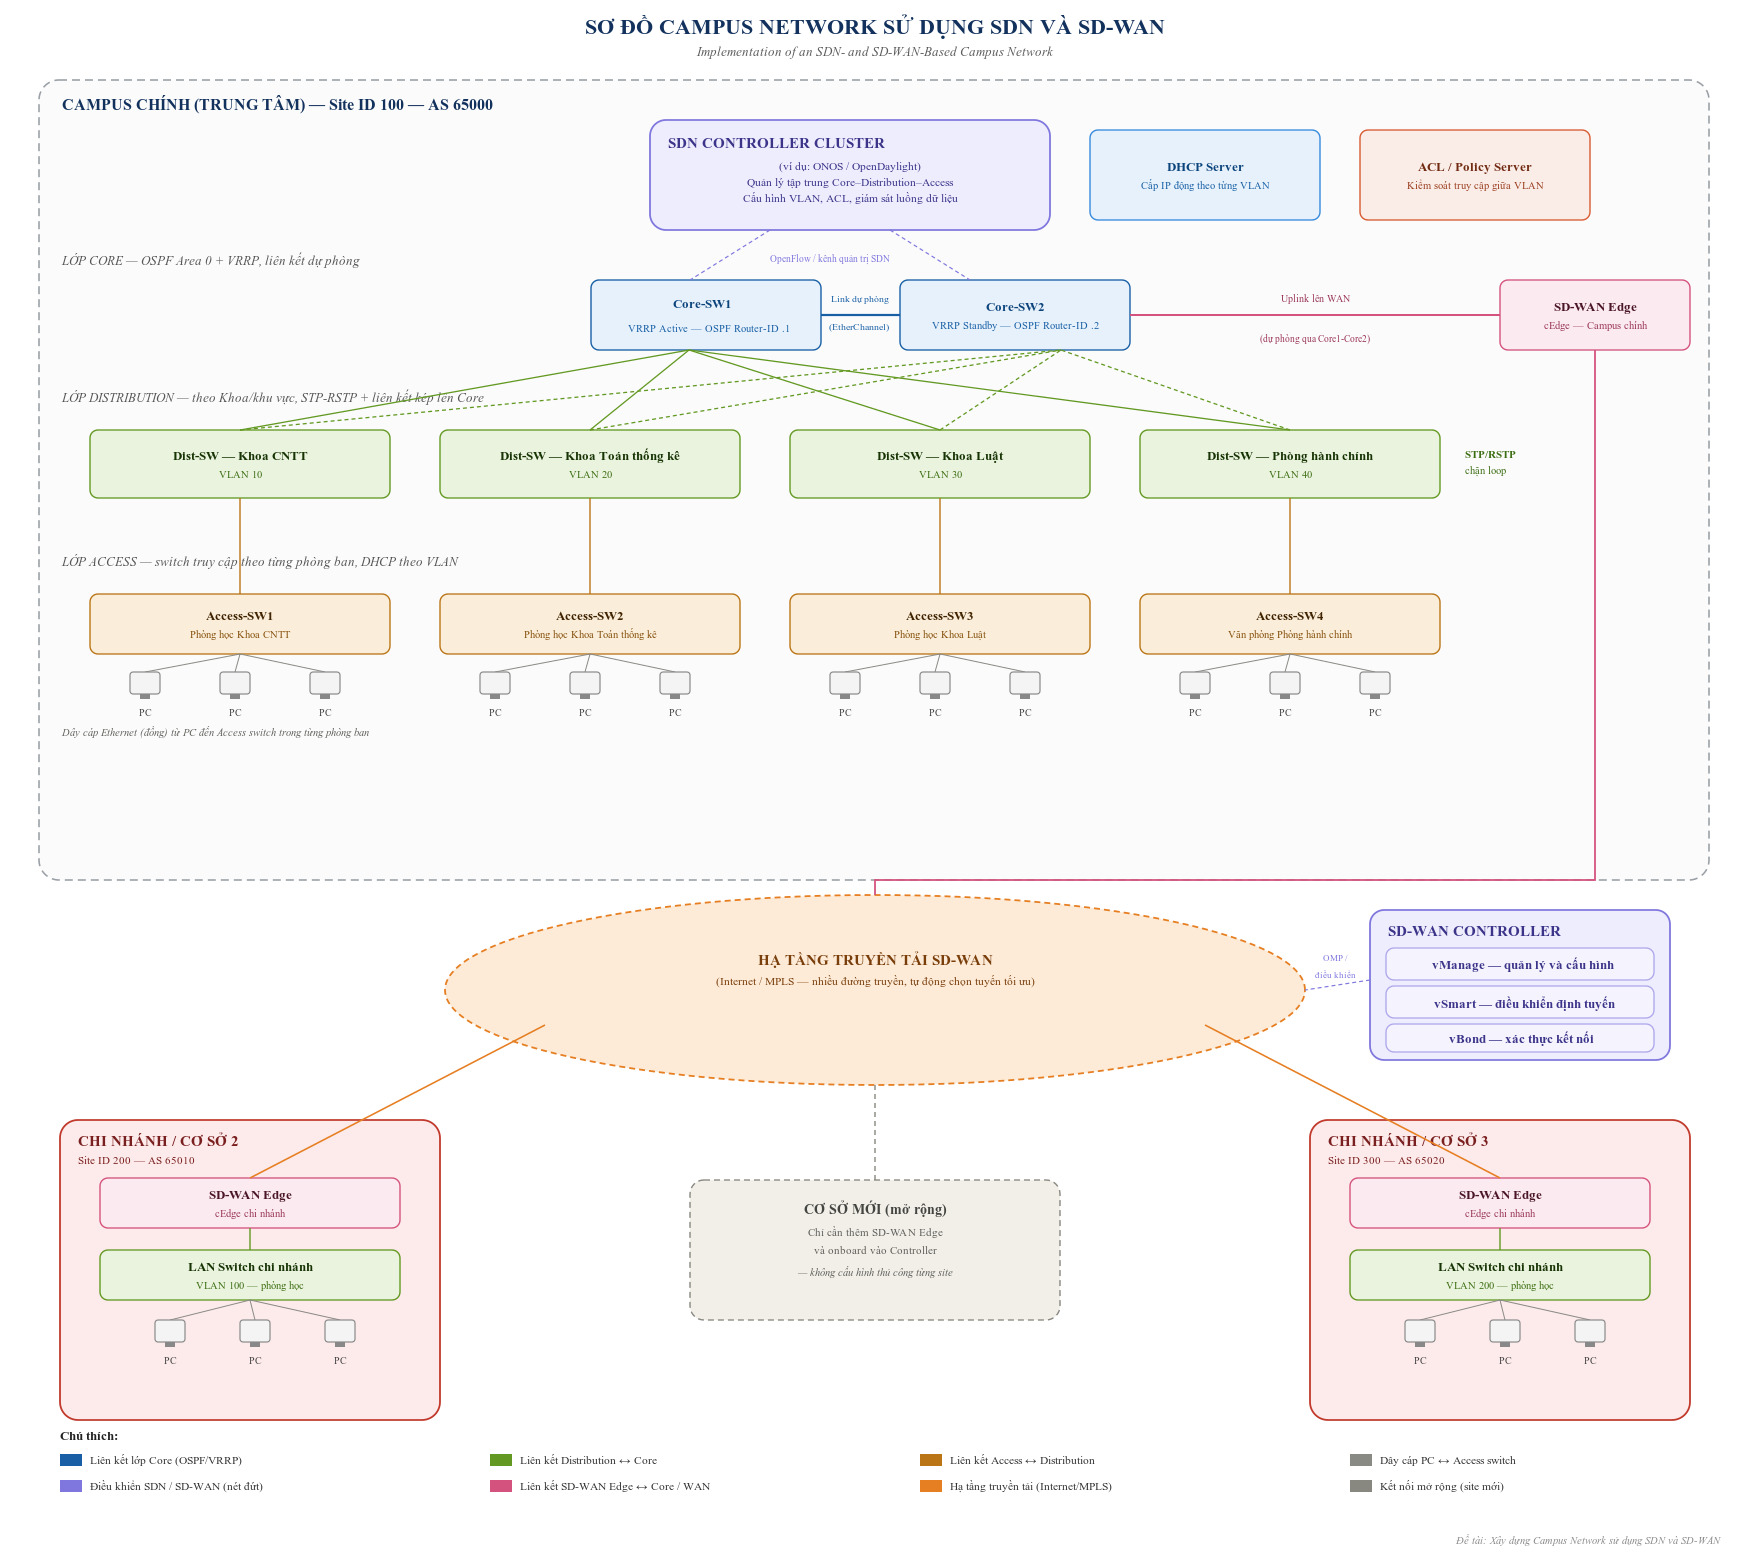
\includegraphics[width=0.90\textwidth]{image/campus_network.jpg}
    \caption{Kiến trúc tổng thể mạng Campus đề xuất}
    \label{fig:kien_truc_tong_the_campus}
\end{figure}

Tại Campus chính (Site ID 100, AS 65000), tầng Core gồm hai thiết bị Core-SW1 và Core-SW2 được triển khai theo cơ chế dự phòng. Hai Core Switch sử dụng VRRP để cung cấp một địa chỉ gateway ảo thống nhất cho các mạng phía dưới; trong đó một thiết bị giữ vai trò active và thiết bị còn lại giữ vai trò standby. Giao thức OSPF Area 0 được sử dụng để trao đổi thông tin định tuyến nội bộ và hỗ trợ hội tụ khi topology thay đổi. Liên kết EtherChannel giữa hai Core Switch giúp tăng băng thông, đồng thời duy trì kết nối khi một đường truyền thành viên gặp sự cố. Các kết nối từ tầng Distribution được triển khai dự phòng đến cả hai Core Switch nhằm hạn chế điểm lỗi đơn trong hạ tầng trung tâm.

SDN Controller sử dụng Ryu tại địa chỉ 10.1.99.10 và quản lý sáu switch OVS ở tầng Distribution/Access bằng OpenFlow 1.3. Core-SW1/2 vẫn thực hiện chức năng lớp 3 bằng VRRP và OSPF, không thuộc tập datapath do Ryu điều khiển. Ryu cài flow chuyển mạch theo VLAN, hỗ trợ flow drop để minh họa ACL tập trung và cung cấp REST API cho ứng dụng giám sát. Mô hình hiện dùng một controller; phương án cluster được xem là hướng phát triển nhằm loại bỏ điểm lỗi đơn.

Tầng Distribution gồm Dist-SW1 và Dist-SW2, có nhiệm vụ tập trung lưu lượng lớp 2 từ bốn Access Switch và chuyển các VLAN 10, 20, 30, 40, 90, 99 lên hai Core. Định tuyến liên VLAN được thực hiện tại Core-SW1/2 thay vì trên Distribution. Hai Distribution và bốn Access là OVS do Ryu điều khiển; OVS STP được tắt vì từng chặn frame trước OpenFlow pipeline. Riêng đường bootstrap VLAN 99 được pruning thành cây không vòng lặp để bảo đảm controller luôn reachable trước khi flow reactive được cài.

Tầng Access gồm các Access Switch đặt tại phòng học, phòng máy hoặc khu vực làm việc và kết nối trực tiếp với thiết bị đầu cuối. Cổng kết nối người dùng được gán vào VLAN tương ứng với khoa hoặc phòng ban. Các máy trạm nhận địa chỉ IP động từ DHCP Server theo từng VLAN, trong khi ACL/Policy Server hỗ trợ kiểm soát quyền truy cập giữa các vùng mạng. Nhờ đó, người dùng chỉ có thể truy cập các dịch vụ nội bộ phù hợp với vai trò của mình; các mạng có mức độ tin cậy khác nhau vẫn được phân tách và kiểm soát rõ ràng.

Kết nối giữa Campus chính và các cơ sở phụ được thực hiện qua SD-WAN Edge. Tại Campus chính, SD-WAN Edge kết nối với tầng Core và tham gia vào hạ tầng truyền tải SD-WAN thông qua Internet, MPLS hoặc nhiều đường truyền đồng thời. Hệ thống SD-WAN Controller trong mô hình gồm vManage để quản lý và cấu hình tập trung, vSmart để điều khiển định tuyến và phân phối chính sách, cùng vBond để xác thực thiết bị và hỗ trợ thiết lập mạng overlay. Thông tin định tuyến và chính sách giữa các thành phần được trao đổi thông qua OMP, cho phép quản trị viên điều khiển đường đi WAN từ một điểm quản lý tập trung.

SD-WAN có thể lựa chọn đường truyền dựa trên các chỉ số chất lượng như độ trễ, độ biến thiên trễ và tỷ lệ mất gói. Lưu lượng quan trọng được ưu tiên qua tuyến đáp ứng yêu cầu chất lượng dịch vụ, trong khi các luồng thông thường có thể được phân bổ sang đường truyền còn lại để cân bằng tải. Khi một kết nối WAN suy giảm chất lượng hoặc bị gián đoạn, SD-WAN Edge tự động chuyển lưu lượng sang tuyến phù hợp khác, qua đó duy trì khả năng truy cập giữa các cơ sở.

Các cơ sở phụ tại Site ID 200, 300 và 400 sử dụng kiến trúc rút gọn gồm hai SD-WAN Edge, một Brand-FW và ba switch lớp 2. Brand-FW làm gateway và DHCP Server cho các VLAN nghiệp vụ; cặp vEdge chia sẻ vai trò dự phòng theo transport, trong đó vEdge1 dùng MPLS và vEdge2 dùng Internet. Site 200 dùng VLAN 60/70, Site 300 dùng VLAN 80/90 và Site 400 dùng VLAN 50/60. Cách tổ chức này cho phép tái sử dụng khuôn cấu hình nhưng vẫn giữ subnet, Site ID và ASN độc lập cho từng cơ sở.

Nhìn chung, kiến trúc đề xuất kết hợp ưu điểm của mô hình Campus ba tầng với khả năng điều khiển tập trung của SDN và khả năng tối ưu kết nối liên cơ sở của SD-WAN. Mô hình giúp giảm cấu hình thủ công, chuẩn hóa chính sách, tăng khả năng dự phòng, nâng cao mức độ bảo mật và hỗ trợ mở rộng hệ thống theo nhu cầu phát triển của nhà trường. Đây là cơ sở để triển khai chi tiết topology, phân hoạch VLAN, quy hoạch địa chỉ IP và các chính sách quản lý trong những phần tiếp theo.

\subsection{Thiết kế topology mạng}

Topology chi tiết của hệ thống được xây dựng theo hướng kết hợp mạng Campus phân tầng tại cơ sở chính với mạng overlay SD-WAN kết nối các cơ sở phụ. Thiết kế gồm năm vùng chính: Campus chính tại Site ID 100, Campus Cần Thơ tại Site ID 200, Campus Đà Nẵng tại Site ID 300, Campus Nha Trang tại Site ID 400 và vùng điều khiển SD-WAN tại Site ID 900. Các site được kết nối qua hai hạ tầng truyền tải độc lập là Internet và MPLS, qua đó tạo nhiều đường đi và cho phép hệ thống chuyển tuyến khi một kết nối gặp sự cố. Topology tổng thể được trình bày trong Hình~\ref{fig:topology_mang_campus}.

\begin{figure}[H]
    \centering
    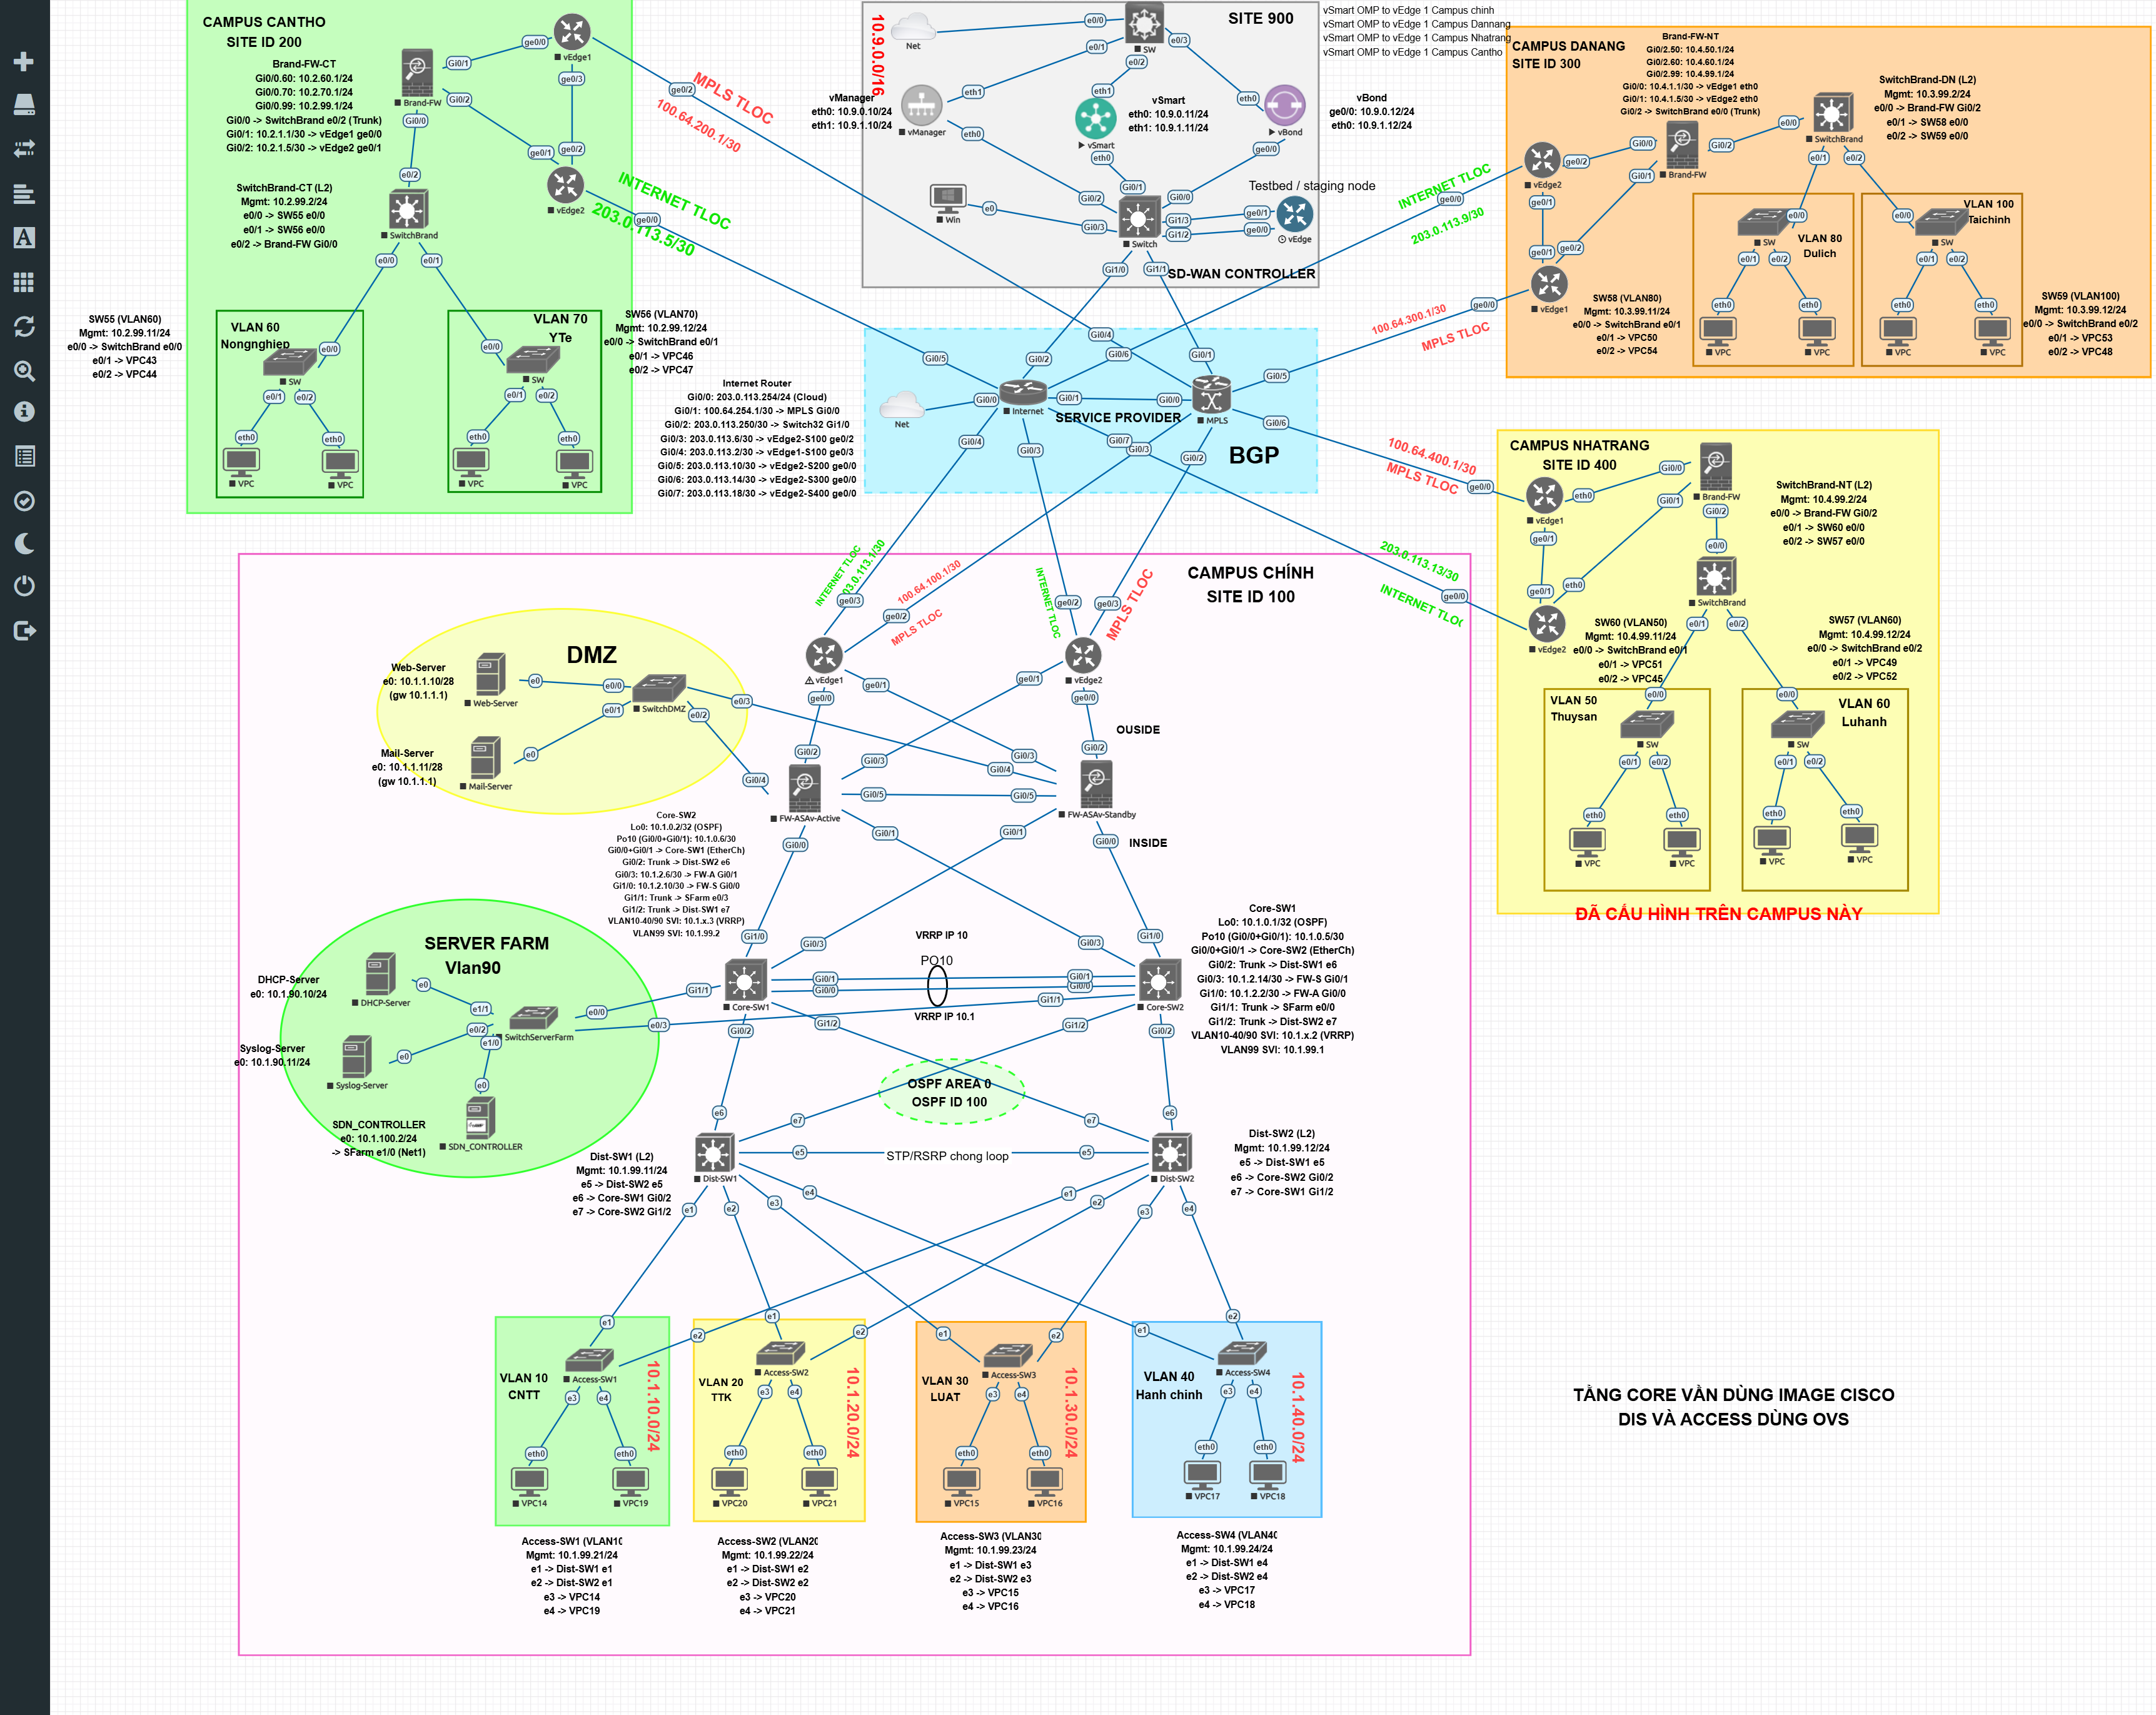
\includegraphics[width=\textwidth]{image/topology.png}
    \caption{Sơ đồ bố trí tổng thể của hệ thống mạng Campus}
    \label{fig:topology_mang_campus}
\end{figure}

\noindent\textit{Lưu ý về hình topology:} các ảnh trong mục này dùng để minh họa bố trí thiết bị và liên kết tại thời điểm thiết kế. Địa chỉ, tên node và cấu hình dùng để triển khai được chốt theo các bảng trong chương, tệp \texttt{Campus Network SDN SD-WAN.unl} và cây \texttt{configs/}; các nguồn dạng văn bản này được ưu tiên khi một nhãn nhỏ trên ảnh chụp cũ chưa được cập nhật.

\subsubsection{Topology tại Campus chính}

\begin{figure}[H]
    \centering
    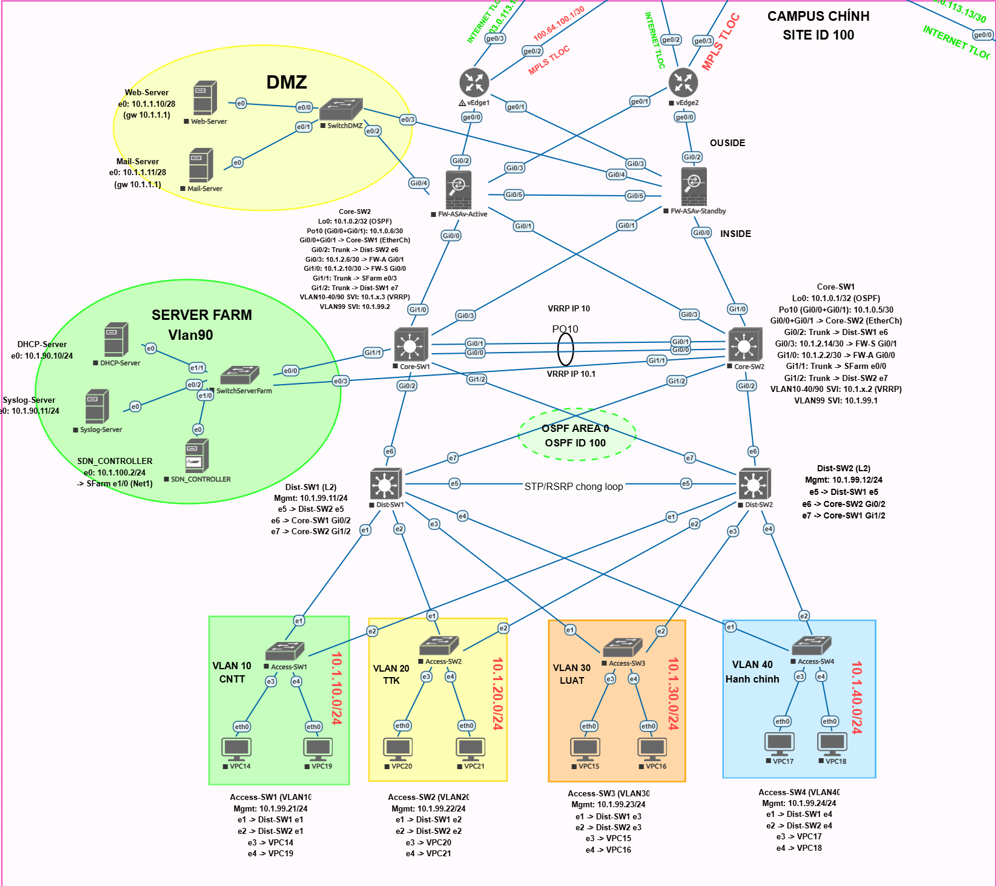
\includegraphics[width=\textwidth]{image/campuschinh.png}
    \caption{Topology chi tiết tại Campus chính}
    \label{fig:topology_campus_chinh}
\end{figure}

Campus chính được triển khai tại Site ID 100 và đóng vai trò trung tâm cung cấp dịch vụ cho toàn hệ thống. Phần LAN sử dụng mô hình Core--Distribution--Access với hai Core Switch, hai Distribution Switch và bốn Access Switch. Hai Core Switch được kết nối trực tiếp với nhau và cung cấp gateway dự phòng thông qua VRRP. Giao thức OSPF Area 0 được sử dụng trên các liên kết lớp 3 giữa Core và các thiết bị hạ tầng liên quan, giúp hệ thống tự động cập nhật đường đi và hội tụ khi một liên kết thay đổi trạng thái.

Hai Distribution Switch được kết nối dự phòng đến cả Core-SW1 và Core-SW2. Từ tầng Distribution, các đường uplink được triển khai xuống nhiều Access Switch để hạn chế ảnh hưởng khi một thiết bị hoặc đường truyền gặp lỗi. Trên sáu OVS, STP được tắt và việc chuyển tiếp do flow OpenFlow của Ryu quyết định; riêng VLAN 99 được pruning thành một cây không vòng lặp để duy trì control plane. Vì vậy khả năng dùng đường dự phòng lớp 2 phải được kiểm tra cùng logic flow, không chỉ dựa vào số lượng uplink vật lý.

Tầng Access được phân chia theo từng khu vực chức năng. Access-SW1 phục vụ VLAN 10 của Khoa Công nghệ thông tin với subnet 10.1.10.0/24; Access-SW2 phục vụ VLAN 20 của Khoa Toán Thống kê với subnet 10.1.20.0/24; Access-SW3 phục vụ VLAN 30 của Khoa Luật với subnet 10.1.30.0/24; và Access-SW4 phục vụ VLAN 40 của khu Hành chính với subnet 10.1.40.0/24. Mỗi Access Switch kết nối trực tiếp các máy trạm và sử dụng cổng trunk trên uplink để chuyển lưu lượng VLAN đến tầng Distribution. Địa chỉ quản trị của các switch được đặt trong một subnet quản trị riêng nhằm tách mặt phẳng quản lý khỏi lưu lượng người dùng.

Vùng Server Farm được kết nối trực tiếp với tầng Core và chứa các dịch vụ dùng chung như DHCP Server, Syslog Server và SDN Controller. DHCP Server được thiết kế cấp phát địa chỉ theo từng VLAN thông qua DHCP Relay đặt trên gateway; Syslog Server thu thập nhật ký từ switch, firewall và các máy chủ; còn SDN Controller quản lý sáu OVS bằng OpenFlow 1.3. Controller nối một cổng vào SwitchServerFarm ở VLAN 99, không sử dụng dây điều khiển riêng đến từng switch.

Các dịch vụ công cộng được bố trí trong vùng DMZ, tách biệt với Server Farm và các VLAN người dùng. Theo sơ đồ, DMZ gồm Web Server và Mail Server kết nối qua một switch riêng đến cặp firewall. Thiết kế này cho phép công bố những dịch vụ cần thiết ra Internet nhưng vẫn ngăn truy cập trực tiếp từ bên ngoài vào mạng nội bộ. Các chính sách NAT, ACL và kiểm tra trạng thái kết nối được áp dụng trên firewall để kiểm soát luồng dữ liệu giữa DMZ, Internet và Campus chính.

Biên mạng Campus chính sử dụng hai firewall hoạt động theo cơ chế active--standby. Phía trong của firewall kết nối dự phòng đến hai Core Switch, phía ngoài kết nối đến hai SD-WAN Edge. Khi firewall active hoặc một liên kết bị lỗi, firewall standby có thể tiếp nhận vai trò xử lý lưu lượng. Hai SD-WAN Edge tại Site 100 được kết nối đến cả Internet và MPLS, tạo các TLOC độc lập cho từng mạng truyền tải. Nhờ đó, Campus chính vừa có dự phòng thiết bị, vừa có dự phòng đường truyền khi trao đổi dữ liệu với các cơ sở phụ.

\subsubsection{Topology vùng điều khiển và mạng truyền tải SD-WAN}

\begin{figure}[H]
    \centering
    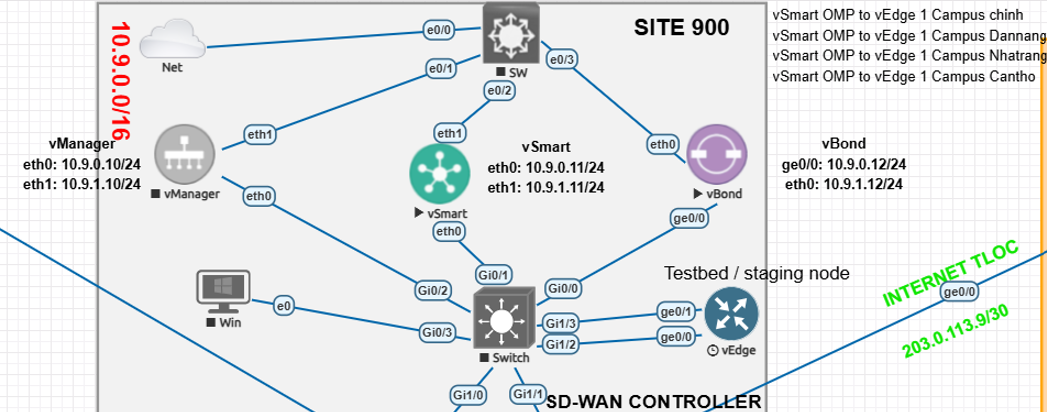
\includegraphics[width=\textwidth]{image/site900.png}
    \caption{Topology vùng điều khiển SD-WAN tại Site 900}
    \label{fig:topology_site900}
\end{figure}

Vùng điều khiển SD-WAN được triển khai tại Site ID 900 với Controller LAN 10.9.0.0/24 và mạng cloud 10.9.1.0/24. Các thành phần chính gồm vManage, vSmart và vBond, cùng máy trạm quản trị và Switch32. vManage cung cấp giao diện cấu hình và giám sát tập trung; vSmart tiếp nhận, xử lý và phân phối thông tin định tuyến OMP; vBond xác thực các SD-WAN Edge và hỗ trợ quá trình thiết lập phiên điều khiển ban đầu. Các thiết bị điều khiển được tách khỏi các VLAN người dùng tại những Campus khác.

Mạng truyền tải được mô phỏng bởi hai miền độc lập. Internet Router thuộc AS 64511, MPLS Router thuộc AS 64512; hai router trao đổi các subnet transit bằng eBGP. Tại Site 100, mỗi vEdge có cả Internet và MPLS TLOC. Tại các chi nhánh, vEdge1 mang MPLS TLOC còn vEdge2 mang Internet TLOC. Trên các kết nối này, Edge thiết lập đường hầm bảo mật đến những Edge khác và gửi thông tin định tuyến lên vSmart thông qua OMP.

Các Controller chỉ tham gia mặt phẳng điều khiển và quản trị, không nằm trực tiếp trên đường đi của lưu lượng người dùng. Sau khi nhận thông tin tuyến và chính sách từ vSmart, các SD-WAN Edge thiết lập đường hầm dữ liệu trực tiếp qua Internet hoặc MPLS. Cách phân tách này giúp tránh việc toàn bộ lưu lượng phải đi qua Controller, đồng thời duy trì khả năng chuyển tiếp trong trường hợp kết nối quản trị tạm thời bị gián đoạn.

\subsubsection{Topology tại các cơ sở phụ}

\begin{figure}[H]
    \centering
    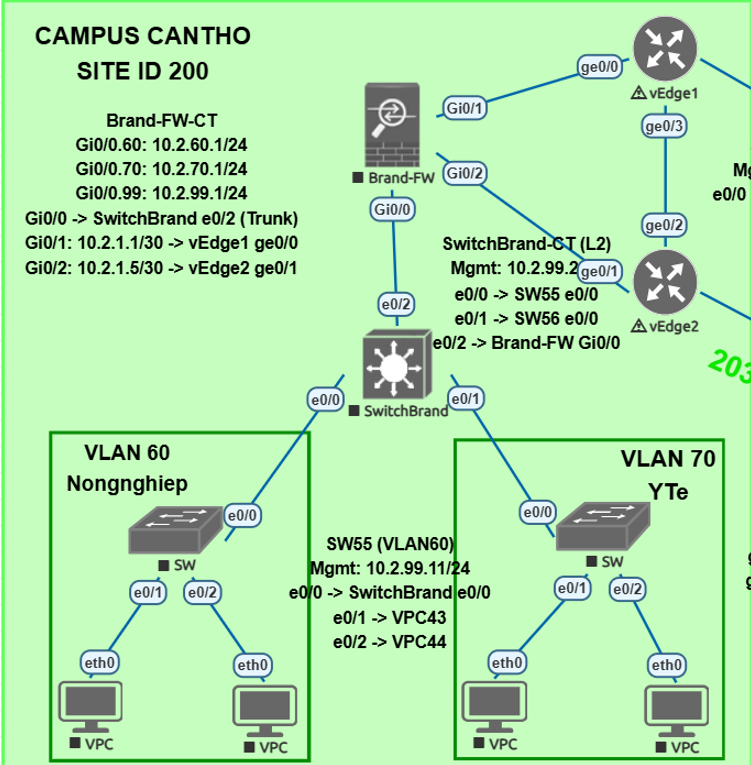
\includegraphics[width=0.72\textwidth]{image/site200.png}
    \caption{Topology Campus Cần Thơ tại Site 200}
    \label{fig:topology_site200}
\end{figure}

Campus Cần Thơ tại Site ID 200 được triển khai với hai SD-WAN Edge, một firewall chi nhánh, một switch tập trung và hai switch truy cập lớp 2. vEdge1 kết nối miền MPLS, còn vEdge2 kết nối miền Internet để cung cấp hai hướng truyền tải độc lập. Phía LAN được chia thành VLAN 60 dành cho khu Nông nghiệp và VLAN 70 dành cho khu Y tế. Các máy trạm kết nối vào switch của từng VLAN, sau đó lưu lượng được tập trung qua switch chi nhánh, firewall và SD-WAN Edge trước khi đi đến Campus chính hoặc Internet.

\begin{figure}[H]
    \centering
    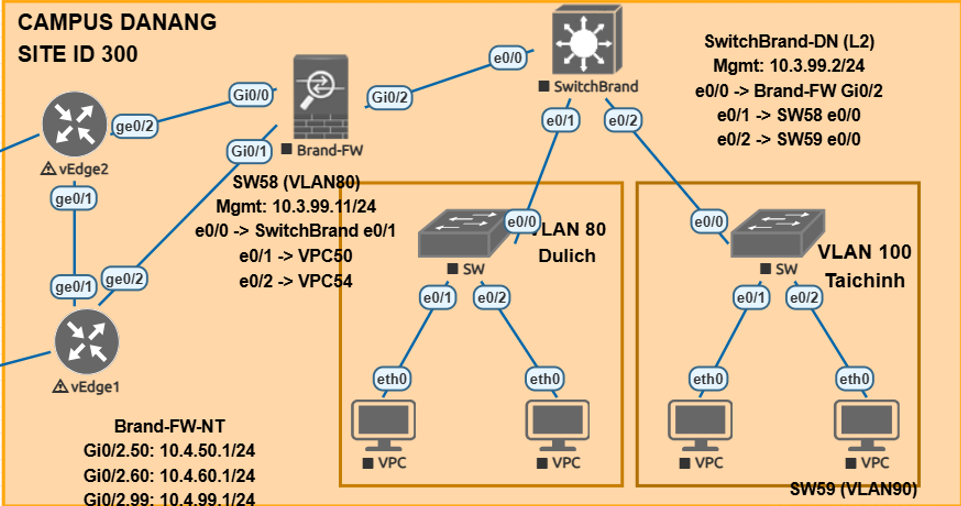
\includegraphics[width=\textwidth]{image/site300.png}
    \caption{Topology Campus Đà Nẵng tại Site 300}
    \label{fig:topology_site300}
\end{figure}

Campus Đà Nẵng tại Site ID 300 có cấu trúc tương tự, gồm hai SD-WAN Edge, firewall chi nhánh, một switch tập trung và hai switch truy cập lớp 2. vEdge1 mang TLOC MPLS, còn vEdge2 mang TLOC Internet. Mạng nội bộ được phân chia thành VLAN 80 cho khu Du lịch và VLAN 90 cho khu Tài chính. Việc tách hai nhóm người dùng thành các VLAN độc lập giúp giới hạn miền quảng bá và tạo điều kiện áp dụng chính sách truy cập khác nhau, đặc biệt đối với VLAN Tài chính có yêu cầu bảo mật cao hơn.

\begin{figure}[H]
    \centering
    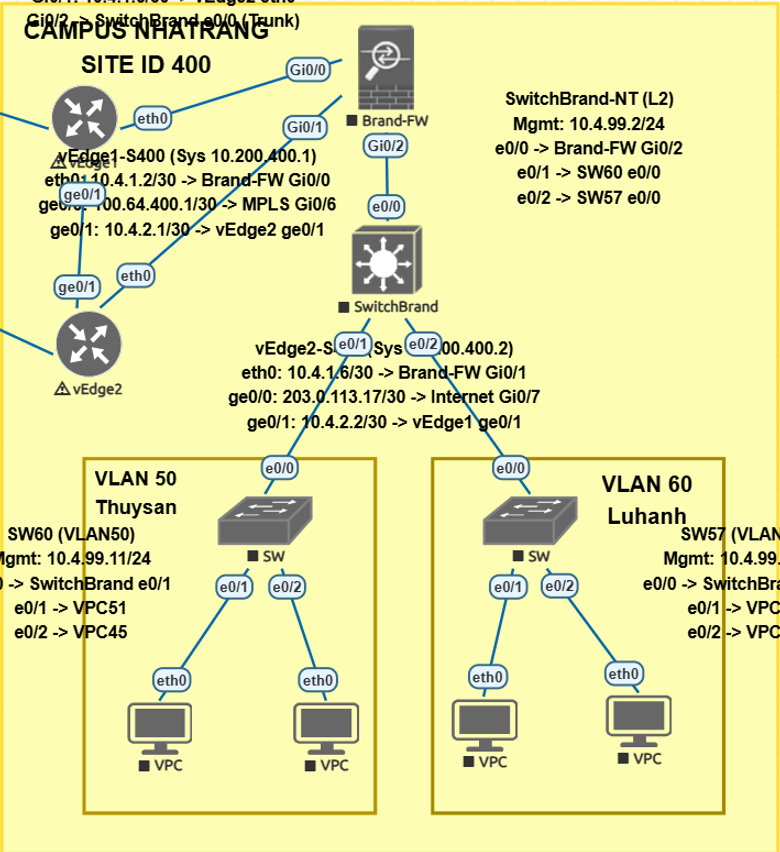
\includegraphics[width=0.72\textwidth]{image/site400.png}
    \caption{Topology Campus Nha Trang tại Site 400}
    \label{fig:topology_site400}
\end{figure}

Campus Nha Trang tại Site ID 400 cũng sử dụng hai SD-WAN Edge, một firewall, một switch tập trung và hai switch truy cập lớp 2. vEdge1 kết nối MPLS, còn vEdge2 kết nối Internet. Phần LAN gồm VLAN 50 cho khu Thủy sản và VLAN 60 cho khu Lữ hành. Switch chi nhánh tập trung các VLAN và chuyển lưu lượng đến firewall trước khi đi qua SD-WAN Edge. Mặc dù VLAN ID có thể được sử dụng lại tại các site khác nhau, các subnet IP của từng cơ sở phải độc lập để tránh trùng lặp khi quảng bá tuyến trên mạng overlay.

Tại các cơ sở phụ, SD-WAN Edge đóng vai trò điểm kết nối giữa mạng LAN và mạng WAN. Edge quảng bá các subnet cục bộ lên vSmart, đồng thời nhận các tuyến được phép đến Server Farm, DMZ hoặc những site khác. Lưu lượng truy cập dịch vụ nội bộ được chuyển qua đường hầm đến Campus chính; lưu lượng Internet thông thường có thể thực hiện local breakout tại chi nhánh nếu đáp ứng chính sách bảo mật. Firewall chi nhánh kiểm soát lưu lượng giữa VLAN người dùng, SD-WAN Edge và Internet, hạn chế việc các máy trạm truy cập trực tiếp vào mặt phẳng quản trị.

\subsubsection{Luồng lưu lượng trong topology}

Đối với lưu lượng nội bộ tại Campus chính, gói tin từ máy trạm đi qua Access Switch, được chuyển đến Distribution Switch và sau đó đến Core Switch. Nếu đích thuộc VLAN khác, việc định tuyến liên VLAN được thực hiện tại cặp Core theo địa chỉ gateway VRRP. Nếu đích là một dịch vụ trong Server Farm, lưu lượng được chuyển trực tiếp từ Core đến vùng máy chủ và chịu sự kiểm soát của ACL. Đối với dịch vụ đặt trong DMZ hoặc tài nguyên bên ngoài Internet, lưu lượng tiếp tục đi qua cặp firewall trước khi đến vùng đích.

Khi người dùng tại cơ sở phụ truy cập dịch vụ ở Campus chính, lưu lượng lần lượt đi từ Access/LAN Switch của chi nhánh đến firewall, SD-WAN Edge và đường hầm overlay. Edge lựa chọn Internet TLOC hoặc MPLS TLOC dựa trên chính sách và chất lượng đường truyền, sau đó chuyển gói tin đến Edge tại Site 100. Tại Campus chính, lưu lượng đi qua firewall và Core để đến Server Farm hoặc VLAN được cấp quyền. Chiều phản hồi sử dụng tuyến overlay tương ứng và vẫn chịu các chính sách bảo mật tại hai đầu kết nối.

Đối với lưu lượng trao đổi giữa hai cơ sở phụ, vSmart quyết định việc phân phối tuyến theo mô hình hub-and-spoke hoặc full-mesh. Nếu chính sách cho phép kết nối trực tiếp, hai Edge có thể thiết lập đường hầm site-to-site để giảm độ trễ. Nếu lưu lượng cần được kiểm tra tập trung, gói tin được chuyển qua Campus chính trước khi đến site đích. Các VLAN người dùng không được mặc định truy cập lẫn nhau; quyền liên lạc phải được xác định rõ trong ACL và chính sách SD-WAN.

\subsubsection{Cơ chế dự phòng và khả năng mở rộng}

Topology sử dụng dự phòng ở nhiều lớp. Tại Campus chính, hệ thống có hai Core Switch, hai Distribution Switch, nhiều uplink chéo, cặp firewall active--standby và hai SD-WAN Edge. Ở lớp 2 OVS, Ryu cài flow và đường management VLAN 99 được pruning để tránh loop; ở lớp 3, OSPF cập nhật tuyến khi liên kết thay đổi; VRRP duy trì gateway mặc định; còn SD-WAN sử dụng BFD và TLOC để chuyển lưu lượng giữa Internet và MPLS. Sự kết hợp này hạn chế điểm lỗi đơn, nhưng từng cơ chế vẫn cần được kiểm thử độc lập.

Các cơ sở phụ cũng được thiết kế với nhiều TLOC và hai SD-WAN Edge, nhờ đó có thể duy trì kết nối khi một thiết bị hoặc một mạng truyền tải bị lỗi. Khi đường MPLS không đáp ứng yêu cầu, lưu lượng có thể chuyển sang Internet; khi đường Internet gặp sự cố, các ứng dụng nội bộ tiếp tục sử dụng MPLS. Việc chuyển tuyến được thực hiện tự động theo trạng thái BFD và chính sách từ vSmart, không yêu cầu quản trị viên cấu hình lại thủ công tại từng site.

Khả năng mở rộng được thực hiện bằng cách bổ sung site, VLAN hoặc Access Switch mới mà không thay đổi cấu trúc cốt lõi. Một cơ sở mới cần được cấp Site ID và System-IP riêng, triển khai SD-WAN Edge, khai báo các subnet LAN và đăng ký chứng thư/chassis/serial với hệ thống controller. Tại Campus chính, VLAN mới phải được bổ sung đồng bộ vào script OVS, trunk Cisco, gateway Core, DHCP và policy Ryu. Thiết kế phân tầng cùng bộ cấu hình theo mẫu giúp hệ thống mở rộng theo từng giai đoạn nhưng vẫn duy trì cấu trúc địa chỉ và cơ chế giám sát thống nhất.

Như vậy, topology đề xuất cung cấp đầy đủ kết nối cho mạng nội bộ Campus, vùng máy chủ, DMZ, hệ thống điều khiển và các cơ sở phụ. Việc kết hợp dự phòng thiết bị, dự phòng liên kết, nhiều mạng truyền tải và điều khiển tập trung giúp hệ thống đạt tính sẵn sàng cao, dễ giám sát và phù hợp với nhu cầu mở rộng của nhà trường trong tương lai.

\subsection{Phân hoạch VLAN và địa chỉ IP}

Phân hoạch VLAN và địa chỉ IP được xây dựng dựa trên cấu trúc site của topology, bảo đảm mỗi khu vực chức năng có một miền quảng bá và một subnet riêng. Toàn bộ mạng nội bộ sử dụng không gian địa chỉ IPv4 private thuộc dải 10.0.0.0/8. Octet thứ hai thể hiện vị trí triển khai: giá trị 1 dành cho Campus chính, 2 dành cho Cần Thơ, 3 dành cho Đà Nẵng, 4 dành cho Nha Trang và 9 dành cho vùng SD-WAN Controller. Cách quy hoạch này giúp quản trị viên xác định nhanh site của một địa chỉ, đồng thời thuận tiện khi tổng hợp tuyến và mở rộng hệ thống.

Các VLAN người dùng và dịch vụ sử dụng subnet /24 để cung cấp đủ địa chỉ cho thiết bị hiện tại và phần dung lượng dự phòng. Địa chỉ kết thúc bằng .1 được ưu tiên làm gateway; tại Campus chính đây là địa chỉ VRRP ảo, còn tại các cơ sở phụ là địa chỉ sub-interface trên Branch Firewall. Các kết nối point-to-point giữa firewall, Core Switch, SD-WAN Edge và router nhà cung cấp sử dụng subnet /30 nhằm tiết kiệm địa chỉ. Loopback dùng cho OSPF và System-IP dùng cho OMP sử dụng prefix /32 vì chỉ đóng vai trò định danh thiết bị.

\subsubsection{Phân hoạch VLAN tại Campus chính}

Campus chính tại Site ID 100 sử dụng các VLAN 10, 20, 30 và 40 cho người dùng; VLAN 90 cho Server Farm; VLAN 99 cho quản trị thiết bị và control plane SDN. DMZ sử dụng một subnet riêng, không dùng chung miền quảng bá với mạng người dùng. Mạng test OpenFlow 10.1.101.0/24 cùng AccessTest/VPC11/VPC12 đã được loại khỏi topology. Quy hoạch VLAN và phạm vi cấp phát DHCP tại Campus chính được trình bày trong Bảng~\ref{tab:vlan_campus_chinh}.

\begin{table}[H]
    \centering
    \small
    \caption{Phân hoạch VLAN tại Campus chính}
    \label{tab:vlan_campus_chinh}
    \begin{tabularx}{\textwidth}{|c|P{2.7cm}|P{2.8cm}|P{2.6cm}|X|}
        \hline
        \textbf{VLAN} & \textbf{Khu vực} & \textbf{Subnet} & \textbf{Gateway} & \textbf{Phạm vi địa chỉ} \\
        \hline
        10 & Khoa Công nghệ thông tin & 10.1.10.0/24 & 10.1.10.1 & DHCP: 10.1.10.100--10.1.10.199 \\
        \hline
        20 & Khoa Toán Thống kê & 10.1.20.0/24 & 10.1.20.1 & DHCP: 10.1.20.100--10.1.20.199 \\
        \hline
        30 & Khoa Luật & 10.1.30.0/24 & 10.1.30.1 & DHCP: 10.1.30.100--10.1.30.199 \\
        \hline
        40 & Phòng Hành chính & 10.1.40.0/24 & 10.1.40.1 & DHCP: 10.1.40.100--10.1.40.199 \\
        \hline
        90 & Server Farm & 10.1.90.0/24 & 10.1.90.1 & Địa chỉ tĩnh cho máy chủ \\
        \hline
        99 & Management & 10.1.99.0/24 & 10.1.99.1 & Địa chỉ tĩnh cho switch và firewall \\
        \hline
    \end{tabularx}
\end{table}

Gateway của các VLAN 10, 20, 30, 40 và 90 được triển khai bằng VRRP trên Core-SW1 và Core-SW2. Core-SW1 sử dụng các địa chỉ SVI kết thúc bằng .2 và giữ vai trò active; Core-SW2 sử dụng các địa chỉ kết thúc bằng .3 và giữ vai trò standby. Ví dụ, tại VLAN 10, hai địa chỉ vật lý là 10.1.10.2 và 10.1.10.3, trong khi máy trạm sử dụng địa chỉ VRRP ảo 10.1.10.1 làm default gateway. Nguyên tắc tương tự được áp dụng cho các VLAN còn lại, giúp người dùng không phải thay đổi gateway khi một Core Switch gặp sự cố.

DHCP Server được đặt tại địa chỉ 10.1.90.10 trong Server Farm. Trên các SVI của VLAN người dùng, địa chỉ helper được cấu hình trỏ về máy chủ này để chuyển tiếp yêu cầu DHCP qua các miền quảng bá. Dải từ .100 đến .199 được dành cho thiết bị đầu cuối; các địa chỉ thấp được ưu tiên cho gateway, switch, máy chủ và thiết bị hạ tầng. VLAN 90 và VLAN 99 không cấp phát động nhằm bảo đảm địa chỉ của máy chủ và thiết bị quản trị luôn ổn định.

Các subnet bổ trợ tại Campus chính được trình bày trong Bảng~\ref{tab:mang_bo_tro_campus}.

\begin{table}[H]
    \centering
    \small
    \caption{Các mạng dịch vụ và hạ tầng tại Campus chính}
    \label{tab:mang_bo_tro_campus}
    \begin{tabularx}{\textwidth}{|P{3.2cm}|P{3.1cm}|X|}
        \hline
        \textbf{Subnet} & \textbf{Chức năng} & \textbf{Địa chỉ hoặc ghi chú chính} \\
        \hline
        10.1.1.0/28 & DMZ & Gateway 10.1.1.1; Web Server 10.1.1.10; Mail Server 10.1.1.11 \\
        \hline
        10.1.90.0/24 & Server Farm & DHCP Server 10.1.90.10; Syslog Server 10.1.90.11 \\
        \hline
        10.1.99.0/24 & Mạng quản trị và SDN & Core .1/.2; SDN Controller .10; Dist .11/.12; Access .21--.24; DMZ .31; Farm .32; firewall .33/.34; PC-Management .50 \\
        \hline
        10.1.0.4/30 & Liên kết hai Core & Core-SW1: 10.1.0.5; Core-SW2: 10.1.0.6 trên Port-Channel 10 \\
        \hline
        10.1.2.0/30, 10.1.2.4/30, 10.1.2.8/30, 10.1.2.12/30 & Firewall--Core & Bốn liên kết point-to-point phía inside \\
        \hline
        10.1.3.0/30, 10.1.3.4/30, 10.1.3.8/30, 10.1.3.12/30 & Firewall--SD-WAN Edge & Bốn liên kết point-to-point phía outside \\
        \hline
        10.1.255.0/29 & Đồng bộ firewall & Mạng failover Gi0/5 giữa firewall active và standby; primary .1, secondary .2 \\
        \hline
    \end{tabularx}
\end{table}

Địa chỉ Loopback0 của Core-SW1 và Core-SW2 lần lượt là 10.1.0.1/32 và 10.1.0.2/32, được sử dụng làm OSPF Router-ID. Trong VLAN quản trị, Core-SW1 và Core-SW2 sử dụng 10.1.99.1 và 10.1.99.2; SDN Controller sử dụng 10.1.99.10; Dist-SW1 và Dist-SW2 sử dụng 10.1.99.11 và 10.1.99.12; bốn Access Switch sử dụng dải 10.1.99.21--10.1.99.24. SwitchDMZ và SwitchServerFarm lần lượt sử dụng 10.1.99.31 và 10.1.99.32; hai firewall dùng 10.1.99.33/.34 trên Management0/0; PC-Management dùng 10.1.99.50. Việc phân nhóm theo vai trò giúp nhận biết nhanh thiết bị khi giám sát và xử lý sự cố.

\subsubsection{Phân hoạch VLAN tại các cơ sở phụ}

Mỗi cơ sở phụ sử dụng octet thứ hai riêng để tránh trùng subnet trên mạng overlay. Các VLAN nghiệp vụ tại chi nhánh được định tuyến bởi sub-interface trên Branch Firewall; VLAN 99 được dành cho quản trị switch. Phân hoạch chi tiết được trình bày trong Bảng~\ref{tab:vlan_chi_nhanh}.

\begin{table}[H]
    \centering
    \small
    \caption{Phân hoạch VLAN tại các cơ sở phụ}
    \label{tab:vlan_chi_nhanh}
    \begin{tabularx}{\textwidth}{|c|c|p{2.5cm}|p{2.5cm}|p{2.3cm}|X|}
        \hline
        \textbf{Site} & \textbf{VLAN} & \textbf{Khu vực} & \textbf{Subnet} & \textbf{Gateway} & \textbf{Phạm vi địa chỉ} \\
        \hline
        200 & 60 & Khoa Nông nghiệp & 10.2.60.0/24 & 10.2.60.1 & DHCP: 10.2.60.100--10.2.60.199 \\
        \hline
        200 & 70 & Khoa Y tế & 10.2.70.0/24 & 10.2.70.1 & DHCP: 10.2.70.100--10.2.70.199 \\
        \hline
        200 & 99 & Management & 10.2.99.0/24 & 10.2.99.1 & Địa chỉ tĩnh \\
        \hline
        300 & 80 & Khoa Du lịch & 10.3.80.0/24 & 10.3.80.1 & DHCP: 10.3.80.100--10.3.80.199 \\
        \hline
        300 & 90 & Khoa Tài chính & 10.3.90.0/24 & 10.3.90.1 & DHCP: 10.3.90.100--10.3.90.199 \\
        \hline
        300 & 99 & Management & 10.3.99.0/24 & 10.3.99.1 & Địa chỉ tĩnh \\
        \hline
        400 & 50 & Khoa Thủy sản & 10.4.50.0/24 & 10.4.50.1 & DHCP: 10.4.50.100--10.4.50.199 \\
        \hline
        400 & 60 & Khoa Lữ hành & 10.4.60.0/24 & 10.4.60.1 & DHCP: 10.4.60.100--10.4.60.199 \\
        \hline
        400 & 99 & Management & 10.4.99.0/24 & 10.4.99.1 & Địa chỉ tĩnh \\
        \hline
    \end{tabularx}
\end{table}

Tại Site 200, SwitchBrand sử dụng địa chỉ quản trị 10.2.99.2; hai Access Switch của VLAN 60 và VLAN 70 sử dụng 10.2.99.11 và 10.2.99.12. Tại Site 300, các địa chỉ tương ứng là 10.3.99.2, 10.3.99.11 và 10.3.99.12. Tại Site 400, SwitchBrand sử dụng 10.4.99.2, còn hai Access Switch sử dụng 10.4.99.11 và 10.4.99.12. Quy luật địa chỉ giống nhau giữa các site giúp chuẩn hóa mẫu cấu hình và thao tác quản trị.

Các liên kết từ Branch Firewall đến hai SD-WAN Edge sử dụng hai subnet /30 thuộc dải 10.x.1.0, trong đó x là số đại diện cho site. Liên kết nội bộ giữa hai Edge sử dụng dải 10.x.2.0/30. Cụ thể, Site 200 dùng 10.2.1.0/30, 10.2.1.4/30 và 10.2.2.0/30; Site 300 dùng 10.3.1.0/30, 10.3.1.4/30 và 10.3.2.0/30; Site 400 dùng 10.4.1.0/30, 10.4.1.4/30 và 10.4.2.0/30. Cách phân chia này tách rõ mạng người dùng khỏi mạng transit và tránh lãng phí địa chỉ trên các liên kết chỉ có hai đầu.

DHCP tại cơ sở phụ được triển khai trực tiếp trên Brand-FW bằng \texttt{dhcpd} theo từng VLAN. Phương án cấp phát cục bộ giúp chi nhánh vẫn cấp được địa chỉ khi kết nối WAN gián đoạn. Trong mô hình, phạm vi .100--.199 được thống nhất cho máy trạm; VLAN 99 tiếp tục sử dụng địa chỉ tĩnh.

\subsubsection{Quy hoạch địa chỉ SD-WAN Controller}

Vùng SD-WAN Controller tại Site ID 900 được chia thành hai subnet riêng. Mạng 10.9.0.0/24 được sử dụng cho Controller LAN, còn mạng 10.9.1.0/24 phục vụ kết nối phía cloud. Switch32 sử dụng địa chỉ 10.9.0.2 làm gateway của Controller LAN; Switch61 sử dụng 10.9.1.1 cho mạng cloud. vManage, vSmart và vBond lần lượt sử dụng các địa chỉ 10.9.0.10, 10.9.0.11 và 10.9.0.12 trên Controller LAN, đồng thời có địa chỉ tương ứng 10.9.1.10, 10.9.1.11 và 10.9.1.12 trên mạng cloud. Máy trạm quản trị sử dụng 10.9.0.20 và chỉ được phép truy cập những giao diện quản lý cần thiết.

vBond được ánh xạ NAT 1:1 ra địa chỉ công cộng 203.0.113.100 để các Edge có thể thực hiện quá trình xác thực và onboard từ mạng truyền tải. vEdge65 tại Site 900 sử dụng địa chỉ LAN 10.9.0.100 và địa chỉ WAN 203.0.113.245/30. Các subnet 203.0.113.248/30 và 100.64.255.248/30 được sử dụng cho kết nối từ vùng Controller đến Internet và MPLS.

\subsubsection{Quy hoạch System-IP và TLOC}

System-IP là địa chỉ /32 dùng để nhận dạng SD-WAN Edge trên mặt phẳng điều khiển OMP, không được sử dụng làm gateway cho mạng LAN. Site 100 và 200 dùng các octet 100 và 200; Site 300, 400 và 900 được rút gọn thành 30, 40 và 90 để octet luôn hợp lệ trong IPv4. TLOC là địa chỉ thuộc mạng underlay, gắn với từng loại đường truyền Internet hoặc MPLS. Quy hoạch chi tiết được trình bày trong Bảng~\ref{tab:system_ip_tloc}.

\begin{table}[H]
    \centering
    \scriptsize
    \caption{Quy hoạch System-IP và TLOC của các SD-WAN Edge}
    \label{tab:system_ip_tloc}
    \begin{tabularx}{\textwidth}{|c|p{1.7cm}|p{2.5cm}|p{3.1cm}|X|}
        \hline
        \textbf{Site} & \textbf{Thiết bị} & \textbf{System-IP} & \textbf{TLOC Internet} & \textbf{TLOC MPLS} \\
        \hline
        100 & vEdge1 & 10.200.100.1/32 & 203.0.113.1/30 & 100.64.100.1/30 \\
        \hline
        100 & vEdge2 & 10.200.100.2/32 & 203.0.113.5/30 & 100.64.100.5/30 \\
        \hline
        200 & vEdge1 & 10.200.200.1/32 & Không sử dụng & 100.64.200.1/30 \\
        \hline
        200 & vEdge2 & 10.200.200.2/32 & 203.0.113.9/30 & Không sử dụng \\
        \hline
        300 & vEdge1 & 10.200.30.1/32 & Không sử dụng & 100.64.30.1/30 \\
        \hline
        300 & vEdge2 & 10.200.30.2/32 & 203.0.113.13/30 & Không sử dụng \\
        \hline
        400 & vEdge1 & 10.200.40.1/32 & Không sử dụng & 100.64.40.1/30 \\
        \hline
        400 & vEdge2 & 10.200.40.2/32 & 203.0.113.17/30 & Không sử dụng \\
        \hline
        900 & vEdge65 & 10.200.90.1/32 & 203.0.113.245/30 & Không sử dụng \\
        \hline
    \end{tabularx}
\end{table}

Mặt Internet sử dụng dải 203.0.113.0/24 và được chia thành các subnet /30 cho từng liên kết Edge--Internet Router. Mặt MPLS sử dụng các subnet 100.64.100.0/30 và 100.64.100.4/30 cho Site 100; 100.64.200.0/30 cho Site 200; 100.64.30.0/30 cho Site 300; và 100.64.40.0/30 cho Site 400. Việc tách riêng hai dải địa chỉ giúp hệ thống nhận biết màu đường truyền và xử lý sự cố độc lập giữa Internet và MPLS.

\subsubsection{Nguyên tắc vận hành và mở rộng địa chỉ}

Các cổng access và trunk trên switch lớp 2 không cấu hình địa chỉ IP trực tiếp; chúng chỉ mang VLAN được chỉ định. Địa chỉ IP chỉ được gán cho SVI quản trị, SVI gateway, cổng định tuyến, Loopback, interface firewall và SD-WAN Edge. Trunk tại Campus chính mang các VLAN 10, 20, 30, 40, 90 và 99; trunk tại chi nhánh mang các VLAN nghiệp vụ của site cùng VLAN 99.

Khi bổ sung một VLAN mới, quản trị viên cần lựa chọn VLAN ID chưa sử dụng trong phạm vi site, cấp một subnet /24 theo quy tắc 10.$<$site$>$.$<$VLAN$>$.0/24 nếu không xảy ra xung đột, dành địa chỉ .1 cho gateway và tạo scope DHCP trong dải .100--.199. Nếu bổ sung site mới, octet thứ hai phải được cấp riêng, System-IP phải duy nhất trên toàn SD-WAN và các subnet TLOC /30 không được trùng với đường truyền hiện có. Tất cả thay đổi phải được cập nhật đồng thời trên DHCP, ACL, OSPF, chính sách OMP và hệ thống giám sát.

Như vậy, phương án phân hoạch VLAN và địa chỉ IP tạo ra cấu trúc rõ ràng giữa mạng người dùng, dịch vụ, quản trị, transit và WAN. Quy tắc địa chỉ thống nhất giúp giảm nguy cơ trùng lặp, hỗ trợ tổng hợp tuyến, đơn giản hóa cấu hình và tạo nền tảng thuận lợi cho việc mở rộng Campus cũng như bổ sung cơ sở mới trong tương lai.

\subsection{Thiết kế quản lý tập trung bằng SDN Controller}

SDN Controller được triển khai tại Site 100 bằng Ryu và sử dụng địa chỉ 10.1.99.10/24. Phạm vi southbound gồm Dist-SW1/2 và Access-SW1--4; hai Core Switch không phải datapath OpenFlow mà tiếp tục đảm nhiệm SVI, VRRP, OSPF và kết nối firewall. Cách phân vai này tạo mô hình Hybrid SDN: Ryu điều khiển lớp 2 OVS, trong khi lớp 3 Cisco giữ các giao thức định tuyến và dự phòng truyền thống.

Control plane OpenFlow 1.3 sử dụng TCP 6653 trên VLAN 99 MANAGEMENT. Controller chỉ cần một liên kết e0 đến SwitchServerFarm e1/0 ở chế độ access VLAN 99. Sáu OVS dùng các địa chỉ 10.1.99.11/.12/.21--.24 và trỏ về cùng controller. Mạng điều khiển cũ 10.1.100.0/24 cùng các dây riêng đã được loại bỏ, do đó thiết kế phản ánh đúng mô hình doanh nghiệp: controller tham gia một management fabric chung thay vì kéo cáp riêng đến từng switch.

Mỗi OVS bridge sử dụng \texttt{fail\_mode=secure}, OpenFlow13 và DPID cố định theo node-id. Ryu cài table-miss flow để frame chưa khớp được gửi lên controller. Ứng dụng \texttt{campus\_switch\_13.py} học MAC theo VLAN, flood trong đúng VLAN và cài flow unicast reactive. Các cổng access được gán VLAN bằng thuộc tính \texttt{tag}; các uplink mang tập VLAN 10, 20, 30, 40, 90 và 99 bằng thuộc tính \texttt{trunks}.

Chính sách bảo mật tập trung được minh họa bằng \texttt{BLOCK\_PORTS}. Khi một cổng được đưa vào danh sách, Ryu cài flow drop priority cao ngay sau khi switch kết nối. Danh sách mặc định để rỗng để tất cả VPCS có thể xin DHCP; khi trình diễn có thể thêm cổng của VPC14 và khởi động lại ứng dụng. Ngoài ra, \texttt{ryu.app.ofctl\_rest} cung cấp REST API trên TCP 8080 để đọc bảng flow hoặc cài flow từ ứng dụng northbound.

Thiết kế giám sát sử dụng một app Ryu riêng để thu PortDescStats và PortStats, tính tốc độ Rx/Tx, tỷ lệ sử dụng cổng và cảnh báo theo ngưỡng. Các endpoint \texttt{/noc/switches}, \texttt{/noc/ports}, \texttt{/noc/congestion}, \texttt{/noc/summary} và dashboard web dùng chung TCP 8080. Đây là phần mở rộng cho phép quan sát tập trung mà không cần cài SNMP agent trên từng OVS.

Vì management reachability cũng đi qua OVS, thiết kế bổ sung flow bootstrap priority 50000 cho VLAN 99 và pruning VLAN 99 thành một cây không vòng lặp. OVS STP được tắt vì từng chặn frame trước OpenFlow pipeline; STP trên phần Cisco vẫn được kiểm tra độc lập. Sau stop/start, service systemd gán lại IP management, controller target, DPID và flow bootstrap; các flow reactive và bảng MAC sẽ được học lại khi có lưu lượng.

SDN Controller và SD-WAN Controller có phạm vi khác nhau. Ryu quản lý lớp 2 trong Site 100; vManage, vSmart và vBond quản lý tám vEdge, route OMP và tunnel giữa các site. Hai miền có thể tích hợp thông qua nền tảng giám sát hoặc API ở giai đoạn sau nhưng không thay thế chức năng của nhau.

Như vậy, thiết kế SDN của đề tài không giả định controller tự động cấu hình toàn bộ Core, VLAN và routing. Mọi thay đổi VLAN vẫn phải đồng bộ giữa script OVS, trunk Cisco, gateway Core, DHCP và policy Ryu. Giá trị chính của SDN trong phạm vi hiện tại là lập trình flow lớp 2, minh họa ACL tập trung, cung cấp API và tập trung hóa dữ liệu giám sát.

\subsection{Thiết kế kết nối các cơ sở bằng SD-WAN}

SD-WAN được sử dụng để kết nối Campus chính với các cơ sở phụ trên một mạng overlay thống nhất, không phụ thuộc vào một loại đường truyền WAN duy nhất. Theo Hình~\ref{fig:kien_truc_tong_the_campus}, Campus chính có Site ID 100, hai cơ sở phụ có Site ID 200 và Site ID 300. Mỗi site được nhận dạng độc lập trên hệ thống Controller, có dải địa chỉ LAN riêng và kết nối vào hạ tầng truyền tải thông qua SD-WAN Edge. Phương án này cho phép nhà trường sử dụng đồng thời Internet và MPLS, đồng thời bổ sung cơ sở mới mà không phải thay đổi cấu trúc mạng tại Campus trung tâm.

Kiến trúc SD-WAN gồm hai thành phần chính là mặt phẳng điều khiển tập trung và mặt phẳng chuyển tiếp phân tán. Mặt phẳng điều khiển bao gồm vManage, vSmart và vBond. vManage cung cấp giao diện quản trị, lưu trữ mẫu cấu hình, giám sát thiết bị và thống kê chất lượng đường truyền. vSmart tiếp nhận thông tin định tuyến từ các SD-WAN Edge, phân phối tuyến và thực thi chính sách điều khiển thông qua OMP. vBond xác thực thiết bị, hỗ trợ các Edge vượt qua cơ chế NAT và cung cấp thông tin cần thiết để thiết lập kết nối ban đầu với các Controller. Mặt phẳng chuyển tiếp gồm các SD-WAN Edge tại từng site, trực tiếp đóng gói, mã hóa và chuyển lưu lượng người dùng qua mạng WAN.

Tại Campus chính, SD-WAN Edge được kết nối dự phòng đến Core-SW1 và Core-SW2. Thiết bị học các mạng nội bộ của Campus thông qua OSPF hoặc các tuyến được công bố từ tầng Core, sau đó quảng bá những tiền tố hợp lệ lên hệ thống SD-WAN. Theo chiều ngược lại, các mạng LAN của cơ sở phụ được SD-WAN Edge chuyển vào bảng định tuyến của Campus chính. Việc lọc và tổng hợp tuyến được thực hiện tại điểm kết nối này nhằm tránh quảng bá các mạng quản trị không cần thiết và hạn chế số lượng tuyến phải duy trì trong toàn hệ thống.

Tại Site ID 200 và Site ID 300, SD-WAN Edge đóng vai trò cổng kết nối giữa mạng LAN chi nhánh và các đường truyền WAN. Phía LAN, Edge kết nối với switch của cơ sở và học các subnet cục bộ bằng tuyến tĩnh hoặc giao thức định tuyến nội bộ. Phía WAN, mỗi Edge được thiết kế với tối thiểu hai kết nối truyền tải, chẳng hạn một đường MPLS và một đường Internet của nhà cung cấp khác. Các giao diện WAN thuộc vùng truyền tải, còn các mạng người dùng được đặt trong vùng dịch vụ riêng. Cách phân tách này giúp chính sách định tuyến, bảo mật và QoS của mạng nội bộ không phụ thuộc trực tiếp vào địa chỉ của nhà cung cấp dịch vụ.

Sau khi được vBond xác thực, SD-WAN Edge thiết lập các phiên điều khiển bảo mật đến vSmart và vManage. vSmart phân phối địa chỉ mạng, thuộc tính đường truyền và chính sách giữa các site thông qua OMP. Từ thông tin nhận được, các Edge thiết lập đường hầm IPsec trực tiếp qua Internet, MPLS hoặc cả hai. Vì lưu lượng dữ liệu được chuyển trực tiếp giữa các Edge nên các Controller không nằm trên đường đi của gói tin người dùng. Khi một Controller tạm thời mất kết nối, các đường hầm và tuyến đã học vẫn có thể tiếp tục được sử dụng trong thời gian hệ thống điều khiển được khôi phục.

Mạng overlay có thể tổ chức theo mô hình hub-and-spoke hoặc full-mesh tùy loại lưu lượng. Campus chính đóng vai trò hub vì tập trung Server Farm, DMZ và các dịch vụ dùng chung. Lưu lượng từ cơ sở phụ đến hệ thống quản lý đào tạo, máy chủ tập tin, DHCP, xác thực hoặc các ứng dụng nội bộ được chuyển về Campus chính. Đối với những dịch vụ cần trao đổi trực tiếp giữa các cơ sở, Controller có thể cho phép tạo đường hầm site-to-site để giảm độ trễ. Các luồng không có nhu cầu liên lạc trực tiếp vẫn được giới hạn theo mô hình hub-and-spoke nhằm đơn giản hóa kiểm soát truy cập.

Chính sách định tuyến ứng dụng được xây dựng dựa trên loại lưu lượng và chất lượng thực tế của từng đường truyền. Các Edge sử dụng BFD để theo dõi độ trễ, độ biến thiên trễ, tỷ lệ mất gói và trạng thái của đường hầm. Controller căn cứ vào các số liệu này để lựa chọn tuyến đáp ứng yêu cầu của ứng dụng. Chính sách đề xuất cho các nhóm lưu lượng được trình bày trong Bảng~\ref{tab:chinh_sach_sla_sdwan}.

\begin{table}[H]
    \centering
    \caption{Chính sách lựa chọn đường truyền SD-WAN đề xuất}
    \label{tab:chinh_sach_sla_sdwan}
    \begin{tabularx}{\textwidth}{|P{3.2cm}|P{4.0cm}|X|}
        \hline
        \textbf{Nhóm lưu lượng} & \textbf{Đường truyền ưu tiên} & \textbf{Nguyên tắc xử lý} \\
        \hline
        Quản lý đào tạo, xác thực và dịch vụ hành chính & MPLS & Ưu tiên tuyến ổn định; chuyển sang Internet khi MPLS không đạt ngưỡng chất lượng hoặc bị gián đoạn. \\
        \hline
        Học trực tuyến, thoại và hội nghị trực tuyến & Tuyến có SLA tốt nhất & Chọn đường có độ trễ, độ biến thiên trễ và tỷ lệ mất gói thấp nhất tại thời điểm truyền. \\
        \hline
        Truy cập Web và dịch vụ Internet thông thường & Internet cục bộ & Thực hiện local breakout tại cơ sở nếu chính sách bảo mật cho phép, tránh chuyển lưu lượng không cần thiết về Campus chính. \\
        \hline
        Sao lưu và truyền tập tin dung lượng lớn & Đường còn băng thông phù hợp & Giới hạn băng thông hoặc lập lịch ngoài giờ cao điểm để không ảnh hưởng đến ứng dụng quan trọng. \\
        \hline
        Mạng khách & Internet cục bộ & Chỉ cho phép truy cập Internet, không quảng bá tuyến đến Server Farm, DMZ và các VLAN nội bộ. \\
        \hline
    \end{tabularx}
\end{table}

Cơ chế local Internet breakout được áp dụng có kiểm soát tại các cơ sở phụ. Lưu lượng truy cập các dịch vụ công cộng có thể đi trực tiếp ra Internet tại site để giảm tải cho đường truyền về Campus chính. Trước khi ra Internet, lưu lượng phải đi qua firewall hoặc chức năng bảo mật tương đương trên SD-WAN Edge. Ngược lại, lưu lượng truy cập Server Farm, vùng quản trị và các ứng dụng nội bộ bắt buộc đi qua mạng overlay đến Campus chính. Việc phân loại được thực hiện dựa trên VPN dịch vụ, subnet nguồn, địa chỉ đích và loại ứng dụng.

Khi một đường truyền WAN gặp sự cố, quy trình chuyển tuyến được thực hiện tự động như sau:

\begin{enumerate}
    \item SD-WAN Edge phát hiện phiên BFD hoặc đường hầm tương ứng không còn đáp ứng điều kiện hoạt động.
    \item Tuyến gắn với đường truyền lỗi bị loại khỏi tập đường đi có thể sử dụng và trạng thái mới được thông báo đến hệ thống điều khiển.
    \item Edge lựa chọn đường hầm còn hoạt động có mức ưu tiên và chất lượng phù hợp với chính sách của ứng dụng.
    \item Lưu lượng được chuyển sang Internet hoặc MPLS còn lại mà không yêu cầu quản trị viên cấu hình lại thủ công.
    \item Khi đường truyền cũ khôi phục và duy trì trạng thái ổn định, hệ thống đưa tuyến trở lại sử dụng theo chính sách đã cấu hình.
\end{enumerate}

Thiết kế cũng dự phòng lỗi thiết bị tại những vị trí quan trọng. Tại Campus chính, SD-WAN Edge có kết nối đến cả hai Core Switch để tránh gián đoạn khi một Core hoặc một liên kết nội bộ gặp sự cố. Trong giai đoạn mở rộng, có thể triển khai cặp Edge hoạt động dự phòng tại Campus chính và các cơ sở có số lượng người dùng lớn. Các Controller được triển khai theo cụm, sử dụng nhiều địa chỉ và đường kết nối khác nhau để hạn chế điểm lỗi đơn trên mặt phẳng điều khiển.

Về bảo mật, mỗi Edge và Controller phải được xác thực bằng chứng thư số trước khi tham gia SD-WAN. Các kênh điều khiển và đường hầm dữ liệu được mã hóa; chỉ các site đã được cấp quyền mới nhận được tuyến và chính sách tương ứng. vManage áp dụng phân quyền theo vai trò, ghi nhật ký thao tác và sao lưu mẫu cấu hình. Chính sách tập trung trên vSmart giới hạn việc trao đổi tuyến giữa các vùng dịch vụ, ngăn mạng khách hoặc subnet không tin cậy truy cập trực tiếp vào tài nguyên nội bộ của nhà trường.

Quá trình bổ sung cơ sở mới được chuẩn hóa bằng mẫu cấu hình. Quản trị viên khai báo Site ID, System IP, các giao diện WAN, subnet LAN và nhóm chính sách trên vManage. Sau khi SD-WAN Edge được kết nối và xác thực, thiết bị tự nhận cấu hình, thiết lập phiên với Controller, học tuyến và hình thành các đường hầm cần thiết. Cơ chế này giúp giảm thời gian triển khai, hạn chế sai lệch cấu hình giữa các cơ sở và cho phép mở rộng hệ thống mà không phải xây dựng lại mạng WAN hiện hữu.

Như vậy, phương án SD-WAN tạo ra một hạ tầng kết nối liên cơ sở có khả năng quản lý tập trung nhưng vẫn chuyển tiếp dữ liệu phân tán tại từng site. Việc kết hợp Internet và MPLS, lựa chọn đường dựa trên chất lượng, local Internet breakout và chuyển tuyến tự động giúp tăng tính sẵn sàng, sử dụng hiệu quả băng thông và bảo đảm các cơ sở phụ truy cập ổn định đến dịch vụ tập trung tại Campus chính.

\subsection{Thiết kế chính sách bảo mật}

Chính sách bảo mật của hệ thống được thiết kế theo nguyên tắc phòng thủ nhiều lớp, kết hợp phân đoạn mạng, kiểm soát truy cập, bảo vệ thiết bị đầu cuối, giám sát tập trung và mã hóa kết nối liên cơ sở. Mục tiêu chính là ngăn truy cập trái phép giữa các nhóm người dùng, hạn chế phạm vi ảnh hưởng khi xảy ra sự cố và vẫn bảo đảm người dùng hợp lệ truy cập được các dịch vụ cần thiết. Chính sách được áp dụng thống nhất tại firewall, Core/Distribution Switch, SDN Controller và SD-WAN Controller thay vì chỉ phụ thuộc vào một thiết bị bảo mật duy nhất.

Nguyên tắc mặc định của hệ thống là từ chối các luồng truy cập không được khai báo rõ ràng. Mỗi VLAN chỉ được phép truy cập những vùng và dịch vụ phù hợp với chức năng của mình. Các ACL được đặt gần nguồn lưu lượng tại tầng Distribution hoặc trên gateway của VLAN để loại bỏ sớm lưu lượng không hợp lệ. Đối với lưu lượng đi Internet, đi qua DMZ hoặc đi giữa Campus chính và cơ sở phụ, firewall và chính sách SD-WAN tiếp tục kiểm tra theo trạng thái kết nối, địa chỉ nguồn, địa chỉ đích, cổng dịch vụ và vùng bảo mật.

Hệ thống được chia thành các vùng bảo mật logic sau:

\begin{itemize}
    \item \textbf{Vùng người dùng:} gồm VLAN 10 của Khoa Công nghệ thông tin, VLAN 20 của Khoa Toán Thống kê và VLAN 30 của Khoa Luật.
    \item \textbf{Vùng hành chính:} VLAN 40 dành cho cán bộ thuộc các phòng ban quản lý và được áp dụng mức kiểm soát cao hơn các VLAN người dùng thông thường.
    \item \textbf{Server Farm:} chứa DHCP Server, máy chủ xác thực, máy chủ tập tin, hệ thống quản lý đào tạo và các dịch vụ nội bộ.
    \item \textbf{DMZ:} chứa các dịch vụ cần công bố ra Internet như Web Server hoặc Mail Server và được tách khỏi mạng nội bộ.
    \item \textbf{Vùng quản trị:} dành cho SDN Controller, hệ thống giám sát, máy trạm quản trị và địa chỉ quản lý của thiết bị mạng.
    \item \textbf{Vùng khách:} phục vụ thiết bị không thuộc quyền quản lý của nhà trường và chỉ được phép truy cập Internet.
    \item \textbf{Vùng WAN:} gồm SD-WAN Edge, các đường truyền Internet/MPLS và các mạng LAN tại cơ sở phụ.
\end{itemize}

Ma trận truy cập tổng quát giữa các vùng được đề xuất trong Bảng~\ref{tab:ma_tran_truy_cap_bao_mat}. Quyền ``cho phép có điều kiện'' nghĩa là chỉ mở các giao thức, địa chỉ đích và cổng dịch vụ cần thiết; những lưu lượng còn lại vẫn bị từ chối.

\begingroup
\small
\begin{longtable}{|P{2.4cm}|P{2.6cm}|P{2.8cm}|P{5.7cm}|}
        \caption{Ma trận chính sách truy cập giữa các vùng mạng}
        \label{tab:ma_tran_truy_cap_bao_mat} \\
        \hline
        \textbf{Nguồn} & \textbf{Đích} & \textbf{Chính sách} & \textbf{Phạm vi cho phép} \\
        \hline
        \endfirsthead
        \multicolumn{4}{c}{\textit{Bảng~\ref{tab:ma_tran_truy_cap_bao_mat} (tiếp theo)}} \\
        \hline
        \textbf{Nguồn} & \textbf{Đích} & \textbf{Chính sách} & \textbf{Phạm vi cho phép} \\
        \hline
        \endhead
        \hline
        \multicolumn{4}{r}{\textit{Tiếp tục ở trang sau}} \\
        \endfoot
        \hline
        \endlastfoot
        VLAN 10, 20, 30 & Server Farm & Cho phép có điều kiện & Chỉ truy cập DNS, DHCP, xác thực, học trực tuyến, máy chủ tập tin và dịch vụ đào tạo được cấp quyền. \\
        \hline
        VLAN 10, 20, 30 & VLAN 40 & Từ chối & Không cho phép người dùng khởi tạo kết nối trực tiếp đến máy trạm và tài nguyên hành chính. \\
        \hline
        VLAN 10, 20, 30 & Giữa các VLAN người dùng & Từ chối mặc định & Chỉ mở luồng phục vụ học tập hoặc nghiên cứu khi có yêu cầu được phê duyệt. \\
        \hline
        VLAN 40 & Server Farm & Cho phép có điều kiện & Truy cập hệ thống quản lý đào tạo, tài chính, nhân sự và dịch vụ nội bộ theo vai trò. \\
        \hline
        Vùng khách & Mạng nội bộ & Từ chối & Không được truy cập VLAN người dùng, VLAN hành chính, Server Farm, DMZ nội bộ và vùng quản trị. \\
        \hline
        Vùng khách & Internet & Cho phép có kiểm soát & Cho phép Web, DNS và các dịch vụ Internet cần thiết; áp dụng giới hạn băng thông và lọc nội dung nếu có. \\
        \hline
        Internet & DMZ & Cho phép có điều kiện & Chỉ công bố các cổng dịch vụ của Web Server, Mail Server hoặc dịch vụ công cộng đã xác định. \\
        \hline
        DMZ & Mạng nội bộ & Từ chối mặc định & Chỉ mở kết nối đến DNS, xác thực, cơ sở dữ liệu hoặc máy chủ nhật ký nếu ứng dụng thực sự yêu cầu. \\
        \hline
        Máy trạm quản trị & Thiết bị mạng và Controller & Cho phép có điều kiện & Cho phép SSH, HTTPS, SNMPv3, NETCONF hoặc giao thức quản trị đã được mã hóa. \\
        \hline
        Các VLAN khác & Vùng quản trị & Từ chối & Không cho phép người dùng truy cập trực tiếp địa chỉ quản lý của thiết bị và Controller. \\
        \hline
        Cơ sở phụ & Campus chính & Cho phép có điều kiện & Chỉ cho phép truy cập các dịch vụ tập trung tương ứng với vai trò và subnet của từng cơ sở. \\
\end{longtable}
\endgroup

Tại biên mạng Campus chính, firewall được triển khai theo cặp active--standby để kiểm soát lưu lượng giữa mạng nội bộ, DMZ, Internet và SD-WAN Edge. Firewall thực hiện kiểm tra trạng thái kết nối, NAT, lọc theo vùng và ghi nhật ký các phiên bị từ chối. Các dịch vụ công cộng không được đặt trực tiếp trong Server Farm mà được bố trí tại DMZ. Khi công bố dịch vụ ra Internet, chỉ địa chỉ và cổng cần thiết được ánh xạ bằng NAT; giao diện quản trị của máy chủ tuyệt đối không được công bố ra bên ngoài.

Server Farm được bảo vệ bằng ACL theo nguyên tắc quyền tối thiểu. Máy chủ sử dụng địa chỉ IP tĩnh và chỉ chấp nhận kết nối từ các subnet đã được cấp quyền. DHCP Server chỉ nhận yêu cầu chuyển tiếp từ các gateway hợp lệ; máy chủ tập tin và hệ thống quản lý đào tạo kiểm soát thêm quyền người dùng ở tầng ứng dụng. Các máy chủ không được tự do khởi tạo kết nối đến VLAN người dùng, trừ những luồng phục vụ cập nhật, giám sát hoặc quản trị đã được xác định. Lưu lượng quản trị máy chủ chỉ xuất phát từ vùng quản trị và được ghi nhật ký.

Tại tầng Access, các cổng kết nối người dùng được gán cố định vào VLAN phù hợp và áp dụng các cơ chế bảo vệ lớp 2. Những cổng không sử dụng phải bị vô hiệu hóa và đưa vào VLAN cách ly. Port Security hoặc 802.1X được sử dụng để hạn chế thiết bị không hợp lệ; DHCP Snooping ngăn máy chủ DHCP giả mạo; Dynamic ARP Inspection và IP Source Guard giảm nguy cơ giả mạo ARP hoặc địa chỉ IP. BPDU Guard được bật trên cổng người dùng để ngăn thiết bị đầu cuối tác động đến cây STP, trong khi Storm Control hạn chế lưu lượng broadcast, multicast hoặc unicast bất thường.

Đối với mạng Wi-Fi, mỗi SSID được ánh xạ vào một VLAN riêng theo nhóm giảng viên, sinh viên, khách hoặc thiết bị chuyên dụng. Người dùng nội bộ cần được xác thực trước khi truy cập mạng; chính sách truy cập được gắn theo vai trò thay vì chỉ dựa vào mật khẩu dùng chung. SSID khách sử dụng vùng khách độc lập, bật cơ chế cô lập thiết bị nếu phù hợp và chỉ cho phép local Internet breakout qua firewall. Việc tách SSID và VLAN giúp chính sách bảo mật giữa mạng có dây và không dây được áp dụng nhất quán.

Mặt phẳng quản trị của thiết bị mạng được tách khỏi lưu lượng người dùng. Switch, router, firewall, SDN Controller và SD-WAN Controller sử dụng địa chỉ quản trị riêng; chỉ máy trạm quản trị được phép truy cập. Telnet, HTTP và các giao thức quản trị không mã hóa phải bị vô hiệu hóa, thay bằng SSH, HTTPS, SNMPv3 và các API sử dụng TLS. Tài khoản quản trị được phân quyền theo vai trò, sử dụng mật khẩu mạnh hoặc xác thực tập trung và khóa tạm thời khi đăng nhập sai nhiều lần. Cấu hình thiết bị được sao lưu định kỳ và lưu tại vị trí có kiểm soát truy cập.

SDN Controller là thành phần điều khiển quan trọng nên phải được bảo vệ ở cả giao diện northbound và southbound. Kết nối từ Controller đến switch sử dụng kênh được xác thực và mã hóa khi thiết bị hỗ trợ. API quản trị yêu cầu xác thực, phân quyền và giới hạn địa chỉ nguồn; không công bố trực tiếp ra Internet. Cụm Controller được cập nhật bản vá, sao lưu cơ sở dữ liệu và giám sát tính toàn vẹn cấu hình. Mọi thay đổi VLAN, ACL, QoS hoặc bảng luồng đều được ghi lại để phục vụ kiểm tra và khôi phục khi xảy ra cấu hình sai.

Đối với SD-WAN, chỉ Edge có chứng thư số hợp lệ mới được phép tham gia mạng overlay. Kênh điều khiển giữa vManage, vSmart, vBond và các Edge được xác thực; dữ liệu giữa các site được truyền qua đường hầm IPsec. Chính sách trên vSmart chỉ phân phối tuyến cần thiết đến từng VPN dịch vụ, tránh để mạng khách hoặc subnet không tin cậy học được tuyến đến Server Farm và vùng quản trị. Giao diện quản trị của SD-WAN Edge không được truy cập từ mạng truyền tải công cộng, ngoại trừ các phiên điều khiển đã được xác định.

Các giao thức hoạt động tại Core và Distribution cũng được giới hạn trên mặt phẳng điều khiển. OSPF chỉ hình thành quan hệ láng giềng trên các liên kết hạ tầng đã chỉ định và sử dụng xác thực khi nền tảng hỗ trợ. Gói tin VRRP, STP và các giao thức quản lý lớp 2 không được tiếp nhận từ cổng người dùng. ACL bảo vệ control plane giới hạn lưu lượng gửi đến CPU của thiết bị, qua đó giảm nguy cơ quét cổng, tấn công từ chối dịch vụ hoặc tạo phiên định tuyến giả mạo.

Hệ thống giám sát tập trung thu thập nhật ký từ firewall, Core/Distribution Switch, SDN Controller, SD-WAN Edge và các máy chủ quan trọng. Tất cả thiết bị đồng bộ thời gian với NTP để bảo đảm dấu thời gian nhất quán. SNMPv3, syslog và thông tin luồng được sử dụng để theo dõi trạng thái cổng, thay đổi cấu hình, số lần đăng nhập thất bại, lưu lượng bị ACL từ chối và các kết nối bất thường. Các cảnh báo quan trọng gồm thiết bị mất kết nối, xuất hiện DHCP Server lạ, cổng chuyển trạng thái liên tục, lưu lượng tăng đột biến hoặc có nhiều lần truy cập trái phép.

Khi phát hiện thiết bị đầu cuối có dấu hiệu bị xâm nhập, quản trị viên có thể sử dụng SDN Controller để đưa cổng hoặc địa chỉ của thiết bị vào VLAN cách ly. Thiết bị bị cô lập chỉ được phép truy cập máy chủ cập nhật hoặc hệ thống kiểm tra an toàn, không được liên lạc với các VLAN khác. Sau khi nguyên nhân được xác định và thiết bị đáp ứng yêu cầu bảo mật, chính sách cách ly mới được gỡ bỏ. Quy trình này giúp hạn chế mã độc lan truyền trong mạng Campus và giảm thời gian xử lý sự cố.

Chính sách bảo mật phải được rà soát định kỳ và cập nhật khi có VLAN, dịch vụ, cơ sở phụ hoặc nhóm người dùng mới. Các ACL không còn sử dụng cần được loại bỏ; tài khoản quản trị của nhân sự đã thay đổi vị trí phải được thu hồi; chứng thư số và bản sao lưu cấu hình phải được kiểm tra thời hạn và khả năng khôi phục. Đồng thời, nhà trường cần thực hiện kiểm thử định kỳ đối với chính sách liên VLAN, truy cập DMZ, local Internet breakout, mất đường truyền và cơ chế cách ly thiết bị.

Như vậy, thiết kế bảo mật kết hợp phân đoạn VLAN, ACL, firewall, bảo vệ tầng Access, quản trị mã hóa và giám sát tập trung để kiểm soát toàn bộ luồng dữ liệu trong hệ thống. Cách tiếp cận này vừa bảo vệ tài nguyên nội bộ tại Campus chính, vừa duy trì chính sách thống nhất cho mạng Wi-Fi và các cơ sở phụ kết nối qua SD-WAN, đồng thời tạo điều kiện mở rộng hệ thống mà không làm giảm mức độ an toàn chung.

	\newpage

    \section{TRIỂN KHAI, KIỂM THỬ VÀ ĐÁNH GIÁ}\label{sec:trien_khai_danh_gia}

Chương này trình bày quá trình hiện thực mô hình đã thiết kế ở Chương~\ref{sec:mo_hinh_de_xuat} trên EVE-NG, cách đồng bộ cấu hình giữa các thiết bị và kết quả kiểm thử thu được. Kết quả được phân loại thành ba mức: \textit{đã kiểm chứng} khi có bằng chứng từ trạng thái thiết bị hoặc phép thử thực tế; \textit{đã cấu hình, cần nghiệm thu} khi cấu hình nguồn đã hoàn thành nhưng chưa có phép thử end-to-end tương ứng; và \textit{chưa triển khai} đối với hạng mục mới dừng ở thiết kế. Cách phân loại này giúp tách kết quả thực nghiệm khỏi chức năng dự kiến, đồng thời làm rõ phạm vi hoàn thành của đề tài.

\subsection{Mục tiêu và nguyên tắc triển khai}

Mục tiêu triển khai là xây dựng một topology thống nhất cho bốn site, trong đó Site 100 thể hiện kiến trúc Campus phân tầng và SDN, các Site 200, 300, 400 thể hiện mô hình chi nhánh, còn Site 900 cung cấp mặt phẳng điều khiển SD-WAN. Hai mạng truyền tải Internet và MPLS được mô phỏng độc lập để kiểm tra BGP underlay, điều khiển OMP, đường hầm IPsec và khả năng chuyển tuyến khi một transport bị gián đoạn.

Quá trình triển khai tuân theo các nguyên tắc sau:

\begin{itemize}
    \item Địa chỉ, VLAN, Site ID, System-IP, node-id và ánh xạ cổng phải thống nhất giữa tài liệu thiết kế, file topology \texttt{Campus Network SDN SD-WAN.unl} và thư mục \texttt{configs/}.
    \item Cấu hình tự động được lưu ở file nguồn và đồng thời nhúng dạng Base64 vào file \texttt{.unl}; cấu hình của Linux/OVS, Windows và SD-WAN Controller được triển khai thủ công hoặc bằng service trong máy ảo.
    \item Không đưa tài khoản, mật khẩu hoặc khóa riêng PKI vào báo cáo. Phần PKI chỉ mô tả quy trình tạo CSR, cài Root CA, cài chứng thư và đăng ký serial/chassis.
    \item Mọi phép thử phải ghi rõ điều kiện, kết quả mong đợi, bằng chứng quan sát và giới hạn của phép đo.
\end{itemize}

\subsection{Môi trường triển khai}

\subsubsection{Nền tảng mô phỏng và thành phần phần mềm}

Mô hình được triển khai trên EVE-NG bằng một file topology duy nhất. Kết quả phân tích tự động file topology ghi nhận \textbf{67 node}, \textbf{100 network}, \textbf{51 node bật startup config} và \textbf{51 payload cấu hình nhúng}. Toàn bộ tham chiếu network-id hợp lệ, không có node hoặc network bị treo. Các nền tảng chính được tổng hợp trong Bảng~\ref{tab:nen_tang_trien_khai_ch4}.

\begin{table}[H]
    \centering
    \small
    \caption{Nền tảng sử dụng trong mô hình triển khai}
    \label{tab:nen_tang_trien_khai_ch4}
    \begin{tabularx}{\textwidth}{|P{3.2cm}|P{4.2cm}|X|}
        \hline
        \textbf{Nhóm thành phần} & \textbf{Nền tảng/image} & \textbf{Vai trò trong mô hình} \\
        \hline
        Core và switch Cisco & IOL L2 High Iron 2019 & Core-SW1/2 thực hiện SVI, VRRP, OSPF; các switch còn lại thực hiện trunk/access và quản trị VLAN 99. \\
        \hline
        Firewall & Cisco ASAv 9.20(2)2 & Cặp firewall HA tại Site 100 và Brand-FW theo mô hình Firewall-as-Core tại các chi nhánh. \\
        \hline
        SDN data plane & Ubuntu Linux + Open vSwitch & Dist-SW1/2 và Access-SW1--4, sử dụng OpenFlow 1.3. \\
        \hline
        SDN control plane & Ryu + ứng dụng Python & Học MAC theo VLAN, cài flow, REST northbound và module giám sát NOC thử nghiệm. \\
        \hline
        SD-WAN & Viptela 20.10.1 & vManage, vSmart, vBond và tám vEdge thuộc các Site 100--400. \\
        \hline
        Service Provider & Cisco vIOS 15.7(3)M3 & Hai router Internet và MPLS chạy eBGP underlay. \\
        \hline
        Máy chủ và máy trạm & Windows Server 2012 R2, Windows 7, VPCS & DHCP, Syslog, Web, Mail, quản trị ASDM và các máy trạm kiểm thử. \\
        \hline
    \end{tabularx}
\end{table}

Việc lựa chọn IOL cho Core-SW1/2 khắc phục tình trạng CPU-hog từng xuất hiện với image vIOS-L2 khi các switch OVS phát broadcast trong lúc Core khởi động. Image IOL đang dùng hỗ trợ đồng thời \texttt{switchport}, SVI, \texttt{ip routing}, VRRP và OSPF. Hai lệnh có ý nghĩa quan trọng là \texttt{vtp mode off}, nhằm tránh VLAN database bị ghi đè bởi switch có revision cao hơn, và \texttt{switchport trunk encapsulation dot1q} trước lệnh \texttt{switchport mode trunk}.

\subsubsection{Quản lý nguồn cấu hình}

Các artifact được tổ chức theo vai trò như Bảng~\ref{tab:artifact_trien_khai_ch4}. Cấu trúc này cho phép truy vết từ yêu cầu thiết kế đến cấu hình thực thi và topology.

\begin{table}[H]
    \centering
    \small
    \caption{Nguồn dữ liệu và phương thức triển khai cấu hình}
    \label{tab:artifact_trien_khai_ch4}
    \begin{tabularx}{\textwidth}{|P{4.1cm}|P{4.2cm}|X|}
        \hline
        \textbf{Artifact} & \textbf{Nội dung} & \textbf{Cách sử dụng} \\
        \hline
        \path{campus_network_sdn_sdwan.md} & Quy hoạch IP, VLAN, cổng, ASN và kiến trúc & Nguồn thiết kế để đối chiếu với topology và báo cáo. \\
        \hline
        \texttt{Campus Network SDN SD-WAN.unl} & Node, interface, network và startup config nhúng & Import vào EVE-NG; kiểm tra XML và invariant trước khi triển khai. \\
        \hline
        \texttt{configs/} & Cấu hình IOS/IOL/ASAv/vEdge/VPCS, script OVS/Ryu và service systemd & Nguồn cấu hình có thể tái sử dụng; một số nền tảng cần dán qua console hoặc copy vào guest. \\
        \hline
        \texttt{configs/README.md} & Ánh xạ thiết bị--node-id và thứ tự khởi động & Tránh dán nhầm cấu hình, đặc biệt với node 40/41/42. \\
        \hline
    \end{tabularx}
\end{table}

Đối với node có \texttt{config="1"}, EVE-NG chỉ nạp startup config khi payload tương ứng tồn tại trong phần \texttt{<configs>} của file \texttt{.unl}. Vì vậy chỉ copy file \texttt{config.cfg} vào thư mục node là chưa đủ. Ngược lại, Linux/OVS, Windows, vManage, vSmart và vBond cần bước cấu hình trong guest. Các vEdge cũng cần chú ý quá trình boot đầu và commit cấu hình; việc wipe node có thể làm mất trạng thái runtime và yêu cầu onboard lại.

\subsection{Triển khai mạng LAN tại Campus chính}

\subsubsection{VLAN, trunk và gateway dự phòng}

Tại Site 100, các VLAN người dùng 10, 20, 30 và 40 được mang qua các liên kết trunk giữa Core, Distribution và Access. VLAN 90 phục vụ Server Farm; VLAN 99 dành cho management và control plane SDN. Core-SW1 sử dụng địa chỉ SVI kết thúc bằng \texttt{.2}, Core-SW2 sử dụng \texttt{.3}; địa chỉ \texttt{.1} là VRRP Virtual IP cho VLAN người dùng và VLAN Server Farm.

Đoạn cấu hình rút gọn trong Khối lệnh~\ref{lst:core_vrrp_ch4} minh họa cơ chế gateway và DHCP relay của VLAN 10.

\begin{lstlisting}[style=customcode,caption={Cấu hình SVI, VRRP và DHCP relay trên Core-SW1},label={lst:core_vrrp_ch4}]
interface Vlan10
 ip address 10.1.10.2 255.255.255.0
 vrrp 10 ip 10.1.10.1
 vrrp 10 priority 150
 ip helper-address 10.1.90.10
 no shutdown
!
router ospf 1
 router-id 10.1.0.1
\end{lstlisting}

Hai Core kết nối qua Port-Channel10 thuộc mạng \texttt{10.1.0.4/30}. Bốn liên kết Core--Firewall sử dụng các subnet \texttt{10.1.2.0/30}, \texttt{10.1.2.4/30}, \texttt{10.1.2.8/30} và \texttt{10.1.2.12/30}. OSPF Area 0 trao đổi route giữa Core và firewall active. Kết quả kiểm tra thực tế cho thấy quan hệ OSPF giữa FW-ASAv-Active và hai Core đạt trạng thái Full sau khi sửa đúng ánh xạ cổng E0/3 và E1/0 trên Core-SW1.

\subsubsection{Firewall HA, DMZ và mạng quản trị}

Cặp FW-ASAv tại Site 100 hoạt động active--standby. Node 1 giữ vai trò Primary--Active; node 2 đạt trạng thái Secondary--Standby Ready. Liên kết failover dùng Gi0/5 và subnet \texttt{10.1.255.0/29}. Cùng một khai báo địa chỉ failover được đặt trên cả hai unit để ASAv tự gán địa chỉ theo vai trò, tránh xung đột trong quá trình negotiation.

DMZ sử dụng \texttt{10.1.1.0/28}, trong đó Web Server là \texttt{10.1.1.10}, Mail Server là \texttt{10.1.1.11}, gateway active là \texttt{10.1.1.1}. Mặt quản trị của cặp firewall được đưa vào VLAN 99 với \texttt{10.1.99.33} và \texttt{10.1.99.34}. PC-Management sử dụng \texttt{10.1.99.50/24}, gateway \texttt{10.1.99.1} và đã truy cập được ASDM của firewall active qua HTTPS. Kết quả này chứng minh đường quản trị từ Server Farm đến firewall HA hoạt động độc lập với các VLAN người dùng.

\subsubsection{Dịch vụ Syslog và DHCP Campus}

Syslog Server được đặt tại \texttt{10.1.90.11/24} và chạy Kiwi Syslog trên Windows. Core-SW1/2, SwitchServerFarm và cặp firewall đã được cấu hình gửi syslog qua UDP 514. Phép thử thực tế ghi nhận Syslog Server nhận được log từ firewall và các thiết bị mạng, do đó hạng mục thu thập nhật ký cơ bản được đánh giá là đã hoàn thành.

DHCP Server tại \texttt{10.1.90.10/24} sử dụng Windows Server 2012 R2. Phần mạng đã sẵn sàng: Core-SW1/2 đều có \texttt{ip helper-address 10.1.90.10} trên SVI VLAN 10/20/30/40, và 8 VPCS tại Site 100 đều có startup config \texttt{ip dhcp}. Tuy nhiên role DHCP và bốn scope trên Windows Server chưa có bằng chứng nghiệm thu cuối cùng. Vì vậy báo cáo chỉ ghi nhận \textit{hạ tầng relay đã cấu hình}, không coi cấp phát DHCP tại Campus chính là kết quả hoàn tất.

\subsection{Triển khai mạng LAN tại các cơ sở phụ}

Ba chi nhánh áp dụng cùng một khuôn Firewall-as-Core: Brand-FW làm gateway lớp 3 và DHCP Server; SwitchBrand cùng hai switch phòng ban chỉ làm lớp 2. Mỗi trunk mang hai VLAN nghiệp vụ và VLAN 99. Việc đặt DHCP tại chỗ giúp máy trạm vẫn nhận địa chỉ khi overlay SD-WAN chưa sẵn sàng.

Kết quả cấp phát được tổng hợp trong Bảng~\ref{tab:dhcp_chi_nhanh_ch4}. Các địa chỉ quan sát đều nằm đúng phạm vi \texttt{.100--.199} và gateway đều là địa chỉ \texttt{.1} trên sub-interface của Brand-FW.

\begin{table}[H]
    \centering
    \scriptsize
    \caption{Kết quả kiểm thử DHCP tại các cơ sở phụ}
    \label{tab:dhcp_chi_nhanh_ch4}
    \begin{tabularx}{\textwidth}{|c|c|P{3.0cm}|P{3.0cm}|X|}
        \hline
        \textbf{Site} & \textbf{VLAN} & \textbf{Subnet/Gateway} & \textbf{VPCS kiểm thử} & \textbf{Địa chỉ nhận được} \\
        \hline
        200 & 60 & 10.2.60.0/24; gw .1 & VPC43, VPC44 & 10.2.60.100; 10.2.60.101 \\
        \hline
        200 & 70 & 10.2.70.0/24; gw .1 & VPC46, VPC47 & 10.2.70.100; 10.2.70.101 \\
        \hline
        300 & 80 & 10.3.80.0/24; gw .1 & VPC50, VPC54 & 10.3.80.100; 10.3.80.101 \\
        \hline
        300 & 90 & 10.3.90.0/24; gw .1 & VPC53, VPC48 & 10.3.90.100; 10.3.90.101 \\
        \hline
        400 & 50 & 10.4.50.0/24; gw .1 & VPC51, VPC45 & 10.4.50.100; 10.4.50.101 \\
        \hline
        400 & 60 & 10.4.60.0/24; gw .1 & VPC49, VPC52 & 10.4.60.100; 10.4.60.101 \\
        \hline
    \end{tabularx}
\end{table}

Trong quá trình triển khai, các IOL chi nhánh không phải lúc nào cũng tự nạp đầy đủ trunk config sau khi start. Cấu hình đã được dán lại qua console, sau đó kiểm tra bằng \texttt{show vlan brief}, \texttt{show interfaces trunk} và lưu bằng \texttt{write memory}. Đây là lý do quy trình vận hành phải bao gồm bước xác minh running-config, không chỉ dựa vào cờ startup config trong EVE-NG.

\subsection{Triển khai SDN tại Site 100}

\subsubsection{Kiến trúc control plane}

SDN Controller là node 9, sử dụng địa chỉ \texttt{10.1.99.10/24} trên e0/ens3 và kết nối SwitchServerFarm e1/0 ở chế độ access VLAN 99. Không còn mạng control riêng \texttt{10.1.100.0/24} và không còn AccessTest/VPC11/VPC12. Kênh OpenFlow đi qua chính management fabric hiện có, đến sáu OVS tại tầng Distribution và Access.

Phạm vi điều khiển và DPID được trình bày trong Bảng~\ref{tab:dpid_sdn_ch4}. Hai Core vẫn chạy control plane Cisco truyền thống; Ryu không quản lý Core-SW1/2.

\begin{table}[H]
    \centering
    \small
    \caption{Ánh xạ switch OVS với SDN Controller}
    \label{tab:dpid_sdn_ch4}
    \begin{tabularx}{\textwidth}{|P{2.8cm}|c|P{3.2cm}|X|}
        \hline
        \textbf{Thiết bị} & \textbf{Node ID} & \textbf{DPID} & \textbf{IP quản trị} \\
        \hline
        Dist-SW1 & 5 & 0000000000000005 & 10.1.99.11/24 \\
        \hline
        Dist-SW2 & 8 & 0000000000000008 & 10.1.99.12/24 \\
        \hline
        Access-SW1 & 68 & 0000000000000044 & 10.1.99.21/24 \\
        \hline
        Access-SW2 & 66 & 0000000000000042 & 10.1.99.22/24 \\
        \hline
        Access-SW3 & 70 & 0000000000000046 & 10.1.99.23/24 \\
        \hline
        Access-SW4 & 69 & 0000000000000045 & 10.1.99.24/24 \\
        \hline
    \end{tabularx}
\end{table}

Mỗi bridge \texttt{br0} sử dụng OpenFlow 1.3, trỏ đến \texttt{tcp:10.1.99.10:6653}, đặt \texttt{fail\_mode=secure} và tắt OVS STP. Cấu hình rút gọn được minh họa trong Khối lệnh~\ref{lst:ovs_controller_ch4}.

\begin{lstlisting}[style=customcode,caption={Thiết lập OpenFlow trên một OVS},label={lst:ovs_controller_ch4}]
ovs-vsctl set bridge br0 protocols=OpenFlow13
ovs-vsctl set bridge br0 other_config:datapath-id=0000000000000044
ovs-vsctl set-controller br0 tcp:10.1.99.10:6653
ovs-vsctl set bridge br0 fail_mode=secure
ovs-vsctl set bridge br0 stp_enable=false
\end{lstlisting}

Vì \texttt{fail\_mode=secure} cần flow để chuyển lưu lượng management trước khi controller kết nối, bộ phục hồi cài hai flow bootstrap priority 50000 cho VLAN 99. Các nhánh mang VLAN 99 được pruning thành một cây không vòng lặp; các VLAN dữ liệu vẫn được giữ trên trunk. Cách làm này giải quyết vòng phụ thuộc ``switch cần controller để forward nhưng controller chỉ reachable qua switch''.

\subsubsection{Ứng dụng Ryu và giám sát}

Ứng dụng \texttt{campus\_switch\_13.py} thực hiện ba chức năng chính:

\begin{enumerate}
    \item Học địa chỉ MAC theo cặp (VLAN, MAC), flood trong đúng VLAN và cài flow unicast reactive.
    \item Cài flow drop proactive cho cổng được khai trong \texttt{BLOCK\_PORTS}. Danh sách mặc định rỗng để không làm gián đoạn DHCP; có thể bật khi demo cách ly VPC14.
    \item Cung cấp REST API qua \texttt{ryu.app.ofctl\_rest} trên TCP 8080 để đọc hoặc thay đổi flow từ ứng dụng northbound.
\end{enumerate}

Mã giám sát NOC được cài trong tệp \path{campus_noc_monitor.py}. Thành phần này thu hai loại thống kê cổng là PortStats và PortDescStats, công bố các endpoint \texttt{/noc/*} và dashboard tại \texttt{http://10.1.99.10:8080/}. Module định nghĩa chu kỳ lấy mẫu, lịch sử băng thông và ngưỡng cảnh báo 70\%/90\%. Tuy nhiên hạng mục này mới được xác nhận ở mức mã nguồn và tích hợp lệnh khởi động; chưa có bộ số liệu tải kéo dài để đánh giá độ chính xác của bandwidth/utilization. Vì vậy NOC dashboard được xem là phần mở rộng thử nghiệm, không phải kết quả hiệu năng đã nghiệm thu.

\subsubsection{Kết quả kiểm tra SDN}

Phép kiểm tra control plane ghi nhận đủ sáu địa chỉ quản trị OVS gửi OpenFlow 1.3 echo đến \texttt{10.1.99.10:6653}. REST endpoint \texttt{/stats/switches} phải trả về tập DPID \texttt{\{5, 8, 66, 68, 69, 70\}}; thứ tự phần tử không có ý nghĩa vì phụ thuộc thứ tự TCP handshake. Đây là bằng chứng sáu switch đã kết nối controller. Việc kiểm thử lưu lượng reactive, ACL demo và khả năng phục hồi sau restart OVS cần được lặp lại theo cùng checklist trước mỗi lần trình diễn vì flow runtime và bảng MAC của Ryu không tồn tại sau khi process khởi động lại.

\subsection{Triển khai SD-WAN giữa các cơ sở}

\subsubsection{Controller, PKI và underlay BGP}

Site 900 gồm vManager, vSmart và vBond. Các địa chỉ LAN lần lượt là \texttt{10.9.0.10}, \texttt{10.9.0.11} và \texttt{10.9.0.12}; System-IP của vSmart là \texttt{10.9.0.13} để không trùng địa chỉ interface VPN 0. Mặt cloud sử dụng \texttt{10.9.1.10}, \texttt{10.9.1.11} và \texttt{10.9.1.12}. Switch32 là IOL thực hiện SVI và static routing cho vùng controller.

Thiết bị chỉ được tham gia fabric sau khi hoàn thành chuỗi PKI: tạo CSR trên vEdge, ký bằng Root CA của lab, cài Root CA chain, cài chứng thư thiết bị và đăng ký đúng cặp chassis-number/serial-number trên cả vManage, vBond và vSmart. Thực nghiệm cho thấy thiếu Root CA gây lỗi xác minh chuỗi chứng thư; thiếu allow-list ở vSmart khiến vEdge có thể lên vBond/vManage nhưng không hình thành OMP với vSmart.

Underlay sử dụng hai ASN nhà cung cấp: Internet AS 64511 và MPLS AS 64512. Hai router hình thành eBGP trên \texttt{100.64.254.0/30}. ASN khách hàng là 65000, 65010, 65020 và 65030 tương ứng các Site 100, 200, 300 và 400. ISP dùng \texttt{default-originate} cho CE; vì vậy vEdge học default route động thay cho việc phụ thuộc hoàn toàn vào static default.

\subsubsection{Ánh xạ vEdge, System-IP và TLOC}

Bảng~\ref{tab:vedge_tloc_ch4} là ánh xạ đã đối chiếu giữa node-id, file cấu hình và topology. Site 100 có hai vEdge, mỗi thiết bị đều có Internet và MPLS. Tại mỗi chi nhánh, vEdge1 mang MPLS còn vEdge2 mang Internet; dự phòng ở cấp site được tạo bởi cặp edge và liên kết nội bộ giữa chúng.

\begin{table}[H]
    \centering
    \scriptsize
    \caption{Ánh xạ vEdge, System-IP và TLOC thực tế}
    \label{tab:vedge_tloc_ch4}
    \begin{tabularx}{\textwidth}{|c|P{2.5cm}|c|P{2.7cm}|P{3.2cm}|X|}
        \hline
        \textbf{Site} & \textbf{Thiết bị} & \textbf{Node} & \textbf{System-IP} & \textbf{Internet TLOC} & \textbf{MPLS TLOC} \\
        \hline
        100 & vEdge1-S100 & 28 & 10.200.100.1 & 203.0.113.1/30 & 100.64.100.1/30 \\
        \hline
        100 & vEdge2-S100 & 6 & 10.200.100.2 & 203.0.113.5/30 & 100.64.100.5/30 \\
        \hline
        200 & vEdge1-S200 & 29 & 10.200.200.1 & Không sử dụng & 100.64.200.1/30 \\
        \hline
        200 & vEdge2-S200 & 42 & 10.200.200.2 & 203.0.113.9/30 & Không sử dụng \\
        \hline
        300 & vEdge1-S300 & 30 & 10.200.30.1 & Không sử dụng & 100.64.30.1/30 \\
        \hline
        300 & vEdge2-S300 & 40 & 10.200.30.2 & 203.0.113.13/30 & Không sử dụng \\
        \hline
        400 & vEdge1-S400 & 31 & 10.200.40.1 & Không sử dụng & 100.64.40.1/30 \\
        \hline
        400 & vEdge2-S400 & 41 & 10.200.40.2 & 203.0.113.17/30 & Không sử dụng \\
        \hline
    \end{tabularx}
\end{table}

Node 65 là vEdge phụ tại Site 900, dùng System-IP hợp lệ \texttt{10.200.90.1}, WAN \texttt{203.0.113.245/30} và LAN \texttt{10.9.0.100/24}. Node này không nằm trong tập tám edge được dùng cho kết quả kiểm thử end-to-end ở Bảng~\ref{tab:vedge_tloc_ch4}; do đó không được tính vào tỷ lệ hoàn thành overlay.

Màu TLOC phải khớp transport: \texttt{biz-internet} cho dải \texttt{203.0.113.x} và \texttt{mpls} cho dải \texttt{100.64.x}. Sai lệch màu trên vEdge2-S200/S300/S400 từng làm fabric thiếu TLOC Internet của chi nhánh và khiến các tunnel cross-color down. Sau khi sửa màu và commit, mỗi vEdge chi nhánh khôi phục các phiên BFD phù hợp với thiết kế.

\subsubsection{Kết quả control plane, BFD và failover}

Sau khi hoàn tất PKI và allow-list, vManage ghi nhận 11 thiết bị trong nhóm kiểm thử gồm ba controller và tám vEdge Site 100--400 ở trạng thái reachable/green. OMP peer đạt 8/8 edge. Các phiên eBGP CE--PE trên hai transport đạt Established và underlay đã ping thành công 10/10 gói theo hai chiều giữa Internet và MPLS TLOC.

Trong trạng thái hội tụ sau phép thử failover, mỗi vEdge Site 100 quan sát 9/12 phiên BFD up; mỗi vEdge1 chi nhánh dùng MPLS quan sát 8/8; mỗi vEdge2 chi nhánh dùng Internet quan sát 6/8. Các phiên còn down là tunnel cross-color ở trạng thái dự phòng theo lựa chọn TLOC hiện tại, không phải mất reachability underlay. Vì dashboard tính cả phiên standby, Site 100 hiển thị khoảng 75\% và các chi nhánh khoảng 87,5\%; các tỷ lệ này cần được diễn giải cùng chính sách tunnel, không nên dùng riêng lẻ để kết luận mạng lỗi.

Phép thử mất đường MPLS tại cả hai vEdge Site 100 được thực hiện bằng cách shutdown interface WAN MPLS. Các tunnel cross-color dự phòng chuyển sang up trong khoảng 2 giây và Site 100 duy trì 6/6 phiên đang sử dụng qua Internet. Khi khôi phục interface, phát hiện TLOC MPLS không được quảng bá lại vì VPN 0 thiếu đường cụ thể đến mạng controller qua MPLS. Hai static route \texttt{10.9.0.0/24} qua \texttt{100.64.100.2} và \texttt{100.64.100.6} được bổ sung cho vEdge1/vEdge2-S100; sau khoảng 60 giây, DTLS hai màu, OMP TLOC và BFD MPLS được khôi phục. Kết quả này cho thấy một TLOC chỉ hợp lệ khi chính transport đó có reachability đến controller, không chỉ khi interface và eBGP đã up.

\subsection{Kịch bản kiểm thử và kết quả tổng hợp}

Các kịch bản được xây dựng theo từng lớp để tránh quy kết sai nguyên nhân. Ví dụ, trước khi kiểm tra OMP cần xác nhận IP interface, route underlay, BGP và PKI; trước khi kiểm tra DHCP cần xác nhận VLAN access, trunk, gateway và DHCP Server. Bảng~\ref{tab:kiem_thu_tong_hop_ch4} tổng hợp trạng thái tại thời điểm hoàn thiện báo cáo.

\begingroup
\scriptsize
\setlength{\tabcolsep}{3pt}
\begin{longtable}{|P{0.8cm}|P{2.7cm}|P{3.4cm}|P{2.0cm}|P{3.8cm}|}
    \caption{Tổng hợp kịch bản kiểm thử và bằng chứng}\label{tab:kiem_thu_tong_hop_ch4} \\
    \hline
    \textbf{Mã} & \textbf{Kịch bản} & \textbf{Kết quả mong đợi} & \textbf{Trạng thái} & \textbf{Bằng chứng/ghi chú} \\
    \hline
    \endfirsthead
    \multicolumn{5}{c}{\textit{Bảng~\ref{tab:kiem_thu_tong_hop_ch4} (tiếp theo)}} \\
    \hline
    \textbf{Mã} & \textbf{Kịch bản} & \textbf{Kết quả mong đợi} & \textbf{Trạng thái} & \textbf{Bằng chứng/ghi chú} \\
    \hline
    \endhead
    \hline
    \endfoot
    T01 & Kiểm tra artifact topology & XML hợp lệ; node/network/config không treo & \textbf{Đạt} & 67 node, 100 network, 51 config bật và 51 payload nhúng; validator không báo lỗi/cảnh báo. \\
    \hline
    T02 & VRRP và OSPF tại Site 100 & Gateway ảo tồn tại; OSPF Full giữa Core và firewall active & \textbf{Đạt} & SVI/VRRP đúng .1/.2/.3; OSPF Full sau khi sửa mapping Core-SW1. \\
    \hline
    T03 & Firewall HA & Primary active, secondary standby ready; config đồng bộ & \textbf{Đạt} & Failover negotiation hoàn tất; ASDM truy cập được từ PC-Management. \\
    \hline
    T04 & DHCP ba chi nhánh & VPCS nhận đúng subnet, gateway .1 và dải .100--.199 & \textbf{Đạt} & 12 VPCS nhận địa chỉ như Bảng~\ref{tab:dhcp_chi_nhanh_ch4}. \\
    \hline
    T05 & DHCP Campus chính & 8 VPCS Site 100 nhận lease qua relay & \textbf{Chưa nghiệm thu} & Helper đã cấu hình; chưa có bằng chứng role/scope DHCP Server hoàn tất. \\
    \hline
    T06 & Thu thập Syslog & Server nhận log UDP 514 từ thiết bị hạ tầng & \textbf{Đạt} & Kiwi Syslog nhận log; Core, Farm và firewall đã khai logging host. \\
    \hline
    T07 & Kết nối Ryu--OVS & Sáu DPID kết nối OpenFlow 1.3 tới TCP 6653 & \textbf{Đạt} & Ghi nhận echo OpenFlow từ sáu IP quản trị; tập DPID mục tiêu đủ 6. \\
    \hline
    T08 & L2 reactive và ACL SDN & Học MAC theo VLAN; flow drop hoạt động khi bật demo & \textbf{Đạt một phần} & Logic đã có trong app; cần lặp lại ping/flow/ACL trực tiếp trước buổi nghiệm thu. \\
    \hline
    T09 & BGP underlay & eBGP ISP--ISP và CE--PE Established; có default route & \textbf{Đạt} & AS 64511--64512 Established; các vEdge nhận default qua transport tương ứng. \\
    \hline
    T10 & SD-WAN control plane & 8 edge có control connection và OMP & \textbf{Đạt} & 11 thiết bị controller+edge reachable/green; OMP edge 8/8. \\
    \hline
    T11 & Màu TLOC và BFD & Internet=biz-internet; MPLS=mpls; tunnel sử dụng được & \textbf{Đạt} & Sửa màu ở node 40/41/42; BFD active đạt trạng thái dự kiến, tunnel standby được giải thích riêng. \\
    \hline
    T12 & Failover MPLS Site 100 & Lưu lượng chuyển sang Internet và quay lại sau phục hồi & \textbf{Đạt} & Standby cross-color up khoảng 2 giây; bổ sung route controller qua MPLS để phục hồi TLOC sau khi no shutdown. \\
    \hline
    T13 & NOC dashboard và cảnh báo tải & PortStats cập nhật liên tục, cảnh báo đúng ngưỡng & \textbf{Chưa nghiệm thu} & Có mã nguồn, REST và dashboard; chưa có thử tải kéo dài và số liệu đối chứng. \\
    \hline
\end{longtable}
\endgroup

\subsection{Đánh giá kết quả}

\subsubsection{Mức độ đáp ứng yêu cầu chức năng}

Mô hình đã thể hiện được các chức năng cốt lõi: phân đoạn VLAN, gateway dự phòng, OSPF nội bộ, firewall HA, DHCP cục bộ tại chi nhánh, syslog tập trung, điều khiển sáu OVS bằng Ryu và kết nối tám vEdge qua fabric SD-WAN. BGP underlay và PKI giúp mô hình gần với quy trình triển khai doanh nghiệp hơn so với cách dùng static route và chứng thư mặc định.

Tính nhất quán cấu hình được cải thiện nhờ ánh xạ node-id và startup config nhúng. Các lỗi thực tế như đảo cổng Core--Firewall, sai màu TLOC, thiếu \texttt{allow-service bgp}, thiếu address-family và thiếu route tới controller qua MPLS đều được phát hiện bằng cách kiểm tra theo lớp. Những lỗi này đồng thời tạo ra bộ tình huống chẩn đoán có giá trị cho phần bảo vệ đề tài.

\subsubsection{Tính sẵn sàng và khả năng phục hồi}

Site 100 có dự phòng ở nhiều lớp: VRRP cho gateway, OSPF cho định tuyến, ASAv active--standby, hai vEdge và hai transport. Các chi nhánh dùng hai vEdge phân chia Internet/MPLS, Brand-FW cấp DHCP tại chỗ và kết nối overlay đến Site 100. Phép thử failover SD-WAN chứng minh đường dự phòng có thể được kích hoạt nhanh; tuy nhiên con số khoảng 2 giây mới là một quan sát trong lab, chưa phải giá trị trung bình từ nhiều lần lặp.

Ở SDN, service systemd và script phục hồi idempotent giúp gán lại IP management, DPID, controller target và flow bootstrap sau stop/start. Dù vậy Ryu hiện chỉ có một controller, nên process hoặc node controller vẫn là điểm lỗi đơn đối với việc học flow mới. Các flow đã cài có thể còn tồn tại trên OVS, nhưng không nên coi đây là cơ chế HA đầy đủ.

\subsubsection{Hiệu năng và khả năng quan sát}

Đề tài đã xây dựng được cơ chế thu số đếm port qua OpenFlow và dashboard NOC thử nghiệm. Tuy nhiên chưa thực hiện bộ đo có kiểm soát cho throughput, latency, jitter, packet loss, CPU/RAM hoặc thời gian hội tụ qua nhiều lần lặp. Do đó Chương 4 không đưa ra kết luận định lượng về hiệu năng tối đa. Kết quả hiện tại phù hợp để chứng minh tính đúng đắn chức năng và quy trình vận hành, chưa đủ để so sánh hiệu năng với thiết bị vật lý hoặc giải pháp thương mại.

\subsubsection{Khả năng tái lập}

Khả năng tái lập được hỗ trợ bởi một topology duy nhất, bộ cấu hình theo node, bảng node-id, validator và quy trình boot theo nhóm thiết bị. Dù vậy Windows, Linux/OVS, controller Viptela và một số IOL vẫn có bước thủ công. Vì thế kết quả tái lập phụ thuộc vào việc tuân thủ đúng thứ tự boot, kiểm tra running-config và không wipe nhầm node đã onboard. Đây là cơ sở để đề xuất tự động hóa sâu hơn ở Chương~\ref{sec:ket_luan_huong_phat_trien}.

	\newpage

    \section{KẾT LUẬN VÀ HƯỚNG PHÁT TRIỂN}\label{sec:ket_luan_huong_phat_trien}

\subsection{Kết quả đạt được}

Đề tài đã xây dựng được mô hình Campus Network đa cơ sở kết hợp SDN và SD-WAN trên EVE-NG. Mô hình gồm Campus chính tại Site 100, ba cơ sở phụ tại Site 200, 300 và 400, vùng điều khiển Site 900 cùng hai mạng truyền tải Internet/MPLS. Topology hiện có 67 node và 100 network; 51 startup config được nhúng trực tiếp trong file lab và đã vượt qua kiểm tra cấu trúc XML, node-id, network reference và payload Base64.

Tại Campus chính, hệ thống đã triển khai các VLAN người dùng 10/20/30/40, Server Farm VLAN 90 và management VLAN 99. Core-SW1/2 cung cấp gateway VRRP, định tuyến OSPF và DHCP relay. Cặp ASAv hoạt động Primary--Active/Secondary--Standby Ready, vùng DMZ được tách khỏi mạng nội bộ và PC-Management đã truy cập được ASDM qua VLAN 99. Syslog tập trung đã nhận log thực tế từ các thiết bị hạ tầng.

Tại ba cơ sở phụ, mô hình Firewall-as-Core đã được triển khai thống nhất. Brand-FW thực hiện router-on-a-stick và cấp DHCP cho sáu VLAN nghiệp vụ; 12 VPCS nhận đúng địa chỉ trong dải \texttt{.100--.199} và đúng gateway \texttt{.1}. Kết quả này chứng minh khả năng tái sử dụng một khuôn cấu hình cho nhiều site nhưng vẫn duy trì subnet và chính sách độc lập.

Thành phần SDN sử dụng Ryu và OpenFlow 1.3 để quản lý hai Distribution OVS và bốn Access OVS tại Site 100. Control plane chạy trên VLAN 99 thay cho mạng và dây điều khiển riêng. Ứng dụng đã hỗ trợ học MAC theo VLAN, cài flow reactive, flow drop proactive tùy chọn và REST API northbound. Bộ service phục hồi OVS/Ryu sau stop/start và module NOC thử nghiệm cũng đã được xây dựng, tạo nền tảng cho quản trị tập trung và giám sát lưu lượng.

Thành phần SD-WAN đã hoàn thiện underlay eBGP với Internet AS 64511, MPLS AS 64512 và bốn ASN khách hàng. Quy trình PKI/allow-list được áp dụng cho tám vEdge thuộc Site 100--400; vManage ghi nhận ba controller và tám edge reachable, OMP đạt 8/8 edge. Các lỗi sai màu TLOC, thiếu BGP service/address-family và thiếu route tới controller qua MPLS đã được khắc phục. Phép thử mất MPLS tại Site 100 quan sát đường dự phòng chuyển sang hoạt động trong khoảng 2 giây và duy trì kết nối qua Internet.

Quan trọng hơn, đề tài đã hình thành được một quy trình kiểm tra theo lớp: topology và startup config; VLAN/trunk/gateway; OSPF/BGP underlay; PKI và control connection; OMP/TLOC/BFD; sau cùng mới kiểm thử dịch vụ đầu cuối. Quy trình này giúp tránh sửa sai tầng và có thể dùng như tài liệu vận hành, xử lý sự cố cho mô hình.

\subsection{Hạn chế của đề tài}

Mặc dù các chức năng chính đã được triển khai, mô hình vẫn còn một số giới hạn:

\begin{itemize}
    \item DHCP tại Campus chính mới hoàn thành phần relay trên Core; role và bốn scope trên Windows Server chưa có bằng chứng nghiệm thu cuối cùng. Vì vậy tám VPCS Site 100 chưa được tính là đã kiểm thử DHCP thành công.
    \item Module NOC đã có mã nguồn, REST API và dashboard nhưng chưa được thử tải kéo dài, chưa đối chứng số liệu với công cụ đo độc lập và chưa lưu dữ liệu lịch sử vào cơ sở dữ liệu bền vững.
    \item SDN Controller hiện là một node Ryu đơn. Service tự khởi động giúp phục hồi sau reboot nhưng không loại bỏ điểm lỗi đơn của control plane.
    \item Logic SDN mới tập trung vào switching theo VLAN và ACL demo. Các chính sách như QoS hoàn chỉnh, topology-aware forwarding, NAC/802.1X, micro-segmentation và xác thực API chưa được hiện thực đầy đủ.
    \item Node vEdge65 ở Site 900 là node phụ/staging và không nằm trong đợt kiểm thử tám edge. Kết quả overlay vì vậy chỉ đại diện cho Site 100--400.
    \item Dashboard SD-WAN vẫn tính các tunnel cross-color standby vào tỷ lệ health. Nếu chỉ nhìn phần trăm mà không xét chính sách TLOC có thể dẫn đến đánh giá sai trạng thái dịch vụ.
    \item Chưa có bộ benchmark lặp nhiều lần cho throughput, latency, jitter, packet loss, thời gian hội tụ, CPU và RAM. Con số failover khoảng 2 giây là kết quả của một tình huống lab, không phải cam kết SLA.
    \item EVE-NG có khác biệt so với thiết bị thật về hiệu năng, clock, console, cơ chế nạp startup config và tài nguyên phần cứng. Nhiều thành phần vẫn cần cấu hình tay, đặc biệt là Windows, Linux/OVS và SD-WAN Controller.
    \item Một số chính sách bảo mật nêu trong Chương 3 mới ở mức thiết kế, chẳng hạn 802.1X, DHCP Snooping, Dynamic ARP Inspection, SNMPv3 và Zero Trust; chưa được tính là kết quả triển khai.
\end{itemize}

\subsection{Hướng phát triển}

Trong giai đoạn tiếp theo, đề tài có thể được phát triển theo các hướng sau:

\begin{enumerate}
    \item \textbf{Hoàn tất dịch vụ Campus chính:} cài role DHCP, tạo và authorize bốn scope, kiểm thử đủ tám VPCS qua relay, sau đó hoàn thiện Web/Mail và ma trận truy cập DMZ--Server Farm--VLAN người dùng.
    \item \textbf{Hoàn thiện NOC:} bảo đảm PortStats được poll định kỳ, kiểm tra công thức bandwidth bằng iPerf, lưu time-series vào cơ sở dữ liệu, đóng gói Chart.js cục bộ và tích hợp cảnh báo qua e-mail hoặc hệ thống ticket.
    \item \textbf{Tăng tính sẵn sàng SDN:} triển khai nhiều controller hoặc nền tảng hỗ trợ cluster, đồng bộ state/flow, bổ sung health-check và kiểm thử mất controller trong khi có lưu lượng mới.
    \item \textbf{Mở rộng chính sách SDN:} phát hiện topology bằng LLDP, tính đường không vòng lặp, triển khai QoS, cách ly endpoint, RBAC cho REST API và ghi audit log cho mọi thay đổi flow.
    \item \textbf{Tối ưu SD-WAN:} chuẩn hóa centralized policy cho TLOC preference, app-route và SLA class; tách rõ tunnel active/standby trên dashboard; lặp phép thử failover Internet/MPLS và mất một vEdge tại từng site.
    \item \textbf{Hoàn thiện Site 900:} quyết định vai trò chính thức của vEdge65, onboard nếu cần làm site staging hoặc loại khỏi topology nếu không phục vụ kịch bản đánh giá.
    \item \textbf{Tự động hóa triển khai:} xây dựng pipeline sinh payload nhúng từ \texttt{configs/}, kiểm tra diff, validate \texttt{.unl}, kiểm tra cú pháp cấu hình và triển khai theo từng node có kiểm soát. Có thể kết hợp Ansible, API EVE-NG và API vManage.
    \item \textbf{Tăng cường bảo mật:} triển khai AAA tập trung, 802.1X/NAC, DHCP Snooping, Dynamic ARP Inspection, SNMPv3, TLS cho kênh quản trị và chính sách Zero Trust giữa các vùng dịch vụ.
    \item \textbf{Thử nghiệm trên thiết bị thật:} chọn một cụm nhỏ gồm Core/Access, firewall và hai đường WAN để đối chiếu hành vi, hiệu năng và thời gian hội tụ với môi trường ảo.
\end{enumerate}

\subsection{Kết luận chung}

Kết quả của đề tài cho thấy SDN và SD-WAN có thể được kết hợp trong một kiến trúc Campus phân tầng mà không làm mất vai trò của các cơ chế truyền thống. VRRP, OSPF, firewall HA và VLAN tiếp tục bảo đảm vận hành cục bộ; Ryu bổ sung khả năng điều khiển và quan sát tập trung cho lớp 2 tại Site 100; còn vManage, vSmart và vBond điều phối kết nối overlay giữa các cơ sở.

Mô hình đã chứng minh được tính khả thi về mặt chức năng và quy trình triển khai. Đồng thời, việc ghi nhận trung thực các hạng mục chưa nghiệm thu cho thấy hệ thống vẫn cần hoàn thiện dịch vụ Campus, giám sát định lượng, tự động hóa và high availability trước khi có thể xem là tương đương một giải pháp production. Đây là nền tảng phù hợp để tiếp tục phát triển thành mô hình thực hành, nghiên cứu và thử nghiệm chính sách mạng Campus đa cơ sở.

	\newpage
        
	% --- PHẦN CUỐI CỦA BÁO CÁO ---
	
	% Tự động tạo TÀI LIỆU THAM KHẢO
	% Lệnh này ép buộc hiển thị TẤT CẢ tài liệu trong file .bib
    \nocite{*}
    \bibliography{tailieuthamkhao}
	
	\newpage
\section*{PHỤ LỤC}
\phantomsection\addcontentsline{toc}{section}{\numberline{} PHỤ LỤC}

\subsection*{A. Mã nguồn topology.py (Trích đoạn chính)}
\begin{lstlisting}[style=customcode, language=Python, caption={Lớp FRRouter -- Thiết bị định tuyến trên Mininet.}]
class FRRouter(Node):
    def config(self, **params):
        super(FRRouter, self).config(**params)
        self.cmd('sysctl -w net.ipv6.conf.all.forwarding=1')
        self.cmd('sysctl -w net.ipv6.fib_multipath_hash_policy=1')
        self.cmd('sysctl -w net.ipv6.conf.all.accept_dad=0')
        confDir = f'/tmp/{self.name}'
        self.cmd(f'rm -rf {confDir} && mkdir -p {confDir}')
        self.cmd(f'/usr/lib/frr/zebra -d -f {confDir}/zebra.conf')
        self.cmd(f'/usr/lib/frr/ospf6d -d -f {confDir}/ospf6d.conf')
\end{lstlisting}

 % Phụ lục mã nguồn
	
\end{document}
